\documentclass[12pt,a4paper]{article}

% Packages
\usepackage[utf8]{inputenc}
\usepackage[T1]{fontenc}
\usepackage{lmodern}
\usepackage[english]{babel}
\usepackage{amsmath,amssymb}
\usepackage{graphicx}
\usepackage{hyperref}
\usepackage{float}
\usepackage{booktabs}
\usepackage[a4paper, left=3cm, right=3cm, top=2cm, bottom=2cm]{geometry}
\usepackage{threeparttable}
\usepackage{multirow}
\usepackage{fancyhdr}
\usepackage{listings}
\usepackage{xcolor}
\usepackage{titlesec}
\usepackage{csquotes}
\usepackage{caption}
\usepackage{pgffor}
\usepackage{acro}
\usepackage{tikz}
\usetikzlibrary{
    shapes.geometric,
    positioning,
    arrows.meta,
    calc,
    fit,
}
\usepackage{mathptmx} % Use Times New Roman font
\usepackage{setspace} % 1.5 line spacing
\usepackage[style=apa, backend=biber]{biblatex}
\addbibresource{references.bib}

% Page layout
\setlength{\parskip}{1em}
\setlength{\parindent}{0em}
\renewcommand{\baselinestretch}{1.5} 

% Section spacing
\titlespacing\section{0pt}{12pt plus 4pt minus 2pt}{0pt plus 2pt minus 2pt}
\titlespacing\subsection{0pt}{12pt plus 4pt minus 2pt}{0pt plus 2pt minus 2pt}
\titlespacing\subsubsection{0pt}{12pt plus 4pt minus 2pt}{0pt plus 2pt minus 2pt}

% Header & Footer
\pagestyle{fancy}
\fancyhf{}
\rhead{\thepage}
\lhead{A Comparison Between Traditional and ML Based Calibration of the 1FHW Model}

% Listings settings
\lstset{
  basicstyle=\ttfamily\small,
  backgroundcolor=\color{gray!10},
  frame=single,
  breaklines=true,
  captionpos=b,
  language=Python
}

\DeclareAcronym{atm}{
    short={ATM},
    long={at-the-money}
}
\DeclareAcronym{otm}{
    short={OTM},
    long={out-of-the-money}
}
\DeclareAcronym{itm}{
    short={ITM},
    long={in-the-money}
}
\DeclareAcronym{otc}{
    short={OTC},
    long={over-the-counter}
}
\DeclareAcronym{hw}{
  short={HW},
  long={Hull-White}
}
\DeclareAcronym{nn}{
  short={NN},
  long={Neural Network}
}
\DeclareAcronym{lmm}{
  short={LMM},
  long={Libor Market Model}
}
\DeclareAcronym{cir}{
    short={CIR},
    long={Cox-Ingersoll-Ross}
}
\DeclareAcronym{gsr}{
    short={GSR},
    long={Gaussian Short Rate}
}
\DeclareAcronym{lm}{
    short={LM},
    long={Levenberg-Marquardt}
}
\DeclareAcronym{sde}{
  short={SDE},
  long={Stochastic Differential Equation}
}
\DeclareAcronym{mse}{
    short={MSE},
    long={Mean Squared Error}
}
\DeclareAcronym{rmse}{
    short={RMSE},
    long={Root Mean Squared Error}
}
\DeclareAcronym{eur}{
    short={EUR},
    long={Euro}
}
\DeclareAcronym{usd}{
    short={USD},
    long={United States Dollar}
}
\DeclareAcronym{vix}{
    short={VIX},
    long={Volatility Index}
}
\DeclareAcronym{move}{
    short={MOVE},
    long={Merrill Lynch Option Volatility Estimate}
}
\DeclareAcronym{pca}{
    short={PCA},
    long={Principal Component Analysis}
}
\DeclareAcronym{bps}{
    short={bps},
    long={Basis Points}
}
\DeclareAcronym{euribor}{
    short={EURIBOR},
    long={Euro Interbank Offer Rate}
}
\DeclareAcronym{libor}{
    short={LIBOR},
    long={London Interbank Offer Rate}
}
\DeclareAcronym{fra}{
    short={FRA},
    long={Forward Rate Agreement}
}
\DeclareAcronym{shap}{
    short={SHAP},
    long={Shapley Additive Explanations}
}
\DeclareAcronym{ai}{
    short={AI},
    long={Artificial Intelligence}
}
\DeclareAcronym{relu}{
    short={ReLU},
    long={Rectified Linear Unit}
}
\DeclareAcronym{tanh}{
    short={tanh},
    long={Hyperbolic Tangent}
}
\DeclareAcronym{api}{
    short={API},
    long={Application Programming Interface}
}

\begin{document}
\onehalfspacing

\begin{titlepage}
	\centering
	% \vspace*{1cm}
	
\includegraphics[width=0.4\textwidth]{images/zhaw_logo.png}
	\vfill
	{\Huge\bfseries A Comparison Between Traditional and Machine Learning Based Calibration of the One Factor Hull-White Model\par}
	{\Large Master's Thesis\par}
	\vspace{1.0cm}
	\vfill
	\begin{minipage}{0.8\textwidth}
		\large
		\begin{tabular}{@{}ll}
			\textbf{Author:}              & Benedikt Grimus    \\
			% \addlinespace[1em]
			\textbf{Matriculation number:} & 1438252            \\
			% \addlinespace[1em]
			\textbf{Study Program:}       & Banking \& Finance \\
			% \addlinespace[1em]
			\textbf{Supervisor:}          & Dr. Marc Weibel    \\
		\end{tabular}
	\end{minipage}
	\vfill
	{\large
		ZHAW School of Management and Law\par
		Submitted on: 18. November 2025\par
	}
	% \vspace*{1cm}
\end{titlepage}
\clearpage

\clearpage
\pagenumbering{gobble}
\section*{Abstract}
The calibration of interest rate models is a cornerstone of quantitative finance, with traditional methods like the \ac{lm} algorithm representing a standard approach. While robust, these methods can be computationally intensive and may, under certain conditions, exhibit parameter instabilities. This thesis addresses these potential limitations by developing and evaluating a \ac{nn} for calibrating the one-factor \ac{hw} model. The research objective is to provide a comparison between this machine learning-based approach and traditional optimization techniques, focusing on out-of-sample pricing accuracy, computational efficiency, and parameter stability. Unlike prior studies that often train \ac{nn} to replicate the outputs of existing optimizers, this thesis implements a framework where the \ac{nn} is trained to directly minimize the pricing error between model-implied and market-observed swaption volatilities.

A \ac{nn} is trained on a dataset of European \ac{atm} swaptions from the \ac{eur} market, covering the period from June to August 2025. The feature set is engineered from yield curve data using \ac{pca} to derive level, slope, and curvature factors, and is augmented with external market indicators. A hold-out set is introduced, which enforces a strict out-of-sample evaluation for both the \ac{nn} and three variations of the \ac{lm} algorithm. Performance is quantified using the \ac{rmse}, calibration runtime, and parameter responses to market shocks.

The results indicate that the \ac{nn}-based approach and the \ac{lm} strategies exhibited distinct performance characteristics within the framework of this study. Regarding out-of-sample pricing accuracy, the \ac{nn} yielded a mean \ac{rmse} of 4.33~\ac{bps}, while the best-performing \ac{lm} strategy resulted in a mean of 6.05~\ac{bps}; the error distribution for the \ac{nn} also showed lower variance across the test period. A substantial difference in computational efficiency was observed. The \ac{nn}, operating as a pre-trained model, performed calibration in approximately 4 milliseconds. In contrast, the \ac{lm} methods, which conduct a full optimization for each market snapshot, required notably more time. In the analysis of parameter dynamics, the \ac{nn}-derived parameters remained stable and responded coherently to simulated market shocks. The parameters calibrated by the \ac{lm} algorithm were observed to be more sensitive to the choice of initialization strategy.

This study concludes that an end-to-end trained \ac{nn} provides a viable framework for the calibration of the one-factor \ac{hw} model, exhibiting favorable characteristics in terms of accuracy, stability, and computational speed under the conditions of this research. The findings suggest that direct error minimization is a promising training paradigm for financial surrogate models, potentially enabling them to identify robust parameter mappings through a global, data-driven learning process.

\textit{JEL Classification: G13, C45}
\clearpage

\pagenumbering{Roman}
\tableofcontents
\clearpage
\newpage

\printacronyms
\newpage

\listoffigures
\newpage

\listoftables
\newpage

\pagenumbering{arabic}
\section{Introduction}
\label{introduction}
Interest rate models are a cornerstone of modern quantitative finance, providing the essential framework for pricing derivatives, managing risk, and formulating hedging strategies. Among the various term structure models, the one-factor Hull-White model has established itself as a benchmark due to its analytical tractability and its ability to perfectly fit the initial term structure of interest rates. Its application is widespread, from the valuation of simple options like caps and floors to more complex, path-dependent instruments such as Bermudan swaptions. However, the utility of any model is fundamentally dependent on its calibration---the process of aligning its parameters with observed market prices to ensure that it reflects current market conditions and expectations.

The calibration of the Hull-White model, particularly its mean-reversion and volatility parameters, presents a significant challenge. Traditional calibration techniques, predominantly based on numerical optimization algorithms like the Levenberg-Marquardt method, are well-established. While effective, these methods often suffer from notable drawbacks. They can be computationally intensive, requiring significant time to converge to a solution. Furthermore, they are susceptible to becoming trapped in local minima, potentially yielding suboptimal parameters that do not accurately represent the global market landscape, especially in volatile or rapidly changing market regimes. This computational latency and potential for instability create a critical bottleneck for financial institutions that require fast and robust model calibrations for real-time pricing and risk management.

The recent advancements in machine learning, and specifically in the field of neural networks, offer a promising alternative to overcome these limitations. Neural networks are exceptionally adept at learning complex, non-linear relationships directly from data. By training a network on historical market data and the corresponding "true" model parameters, it is possible to create a surrogate model that can approximate the calibration function almost instantaneously. This data-driven approach has the potential to transform the calibration process from a time-consuming optimization task into a rapid inference problem, thereby offering significant gains in speed and consistency. The motivation for this research stems from the pressing need for more efficient and robust calibration techniques in an increasingly fast-paced financial world.

The primary aim of this thesis is to provide a comprehensive comparison between the traditional, optimization-based calibration of the one-factor Hull-White model and a modern, machine learning-based approach. To achieve this, the research will be guided by the following key questions:
\begin{enumerate}
    \item How does the accuracy of a neural network-based calibration, measured by the model's ability to replicate market swaption prices, compare to that of the traditional Levenberg-Marquardt algorithm?
    \item What is the quantitative difference in computational speed between the two methods, considering both the initial setup (training) and the ongoing application (inference)?
    \item How stable are the estimated model parameters over time?
\end{enumerate}

To ensure a focused and rigorous analysis, this study is subject to several delimitations. The scope is confined to the one-factor Hull-White model, calibrated using a comprehensive dataset of European at-the-money (ATM) swaptions from the Euro (EUR) market. The analysis covers a continuous time period from June 1, 2025, to August 31, 2025, providing a view of the model's performance in a recent market environment. The study does not extend to multi-factor models or other classes of interest rate derivatives.

This thesis is structured as follows. Chapter \ref{background} provides a detailed background on the theoretical foundations, including swaptions, yield curve bootstrapping, and a thorough review of the Hull-White model and its traditional calibration. Chapter \ref{methodology} delineates the research methodology, covering the dataset, the implementation of the machine learning framework, the feature engineering process, and the metrics used for comparison. Chapter \ref{results} presents the empirical results of the comparative analysis, focusing on accuracy, speed, and robustness. Finally, chapter \ref{conclusion} concludes the thesis by summarizing the key findings, discussing their implications for financial practitioners, and suggesting avenues for future research.
\newpage

\section{Background}
\label{background}
To provide the necessary context for the comparative analysis at the heart of this thesis, this chapter establishes a comprehensive theoretical foundation. The discussion is structured to build from fundamental concepts to specific applications. It begins with an overview of swaptions, detailing their characteristics and significance in the interest rate derivatives market. Following this, the chapter explains the crucial process of bootstrapping the zero-coupon yield curve from swap rates, a foundational step for any term structure model.

With the market instruments defined, the focus shifts to the models governing their dynamics. An introduction to the theory of short-rate models provides the broader context, differentiating between equilibrium and no-arbitrage frameworks. This leads to a detailed examination of the one-factor \ac{hw} model, covering its mathematical specification, analytical solutions for pricing, and the traditional calibration process via numerical optimization techniques such as the \ac{lm} algorithm. Finally, the chapter introduces the core principles of the machine learning approach used in this study, outlining the foundational concepts of \ac{nn}s, including their architecture and learning mechanisms like the back-propagation algorithm, which enable their use as a powerful and modern calibration tool.

\subsection{Swaptions: Definition, Characteristics, and Financial Relevance} \label{swaptions}
A swaption, or swap option, is a derivative contract that grants the holder the right, but not the obligation, to enter into an interest rate swap at a predetermined date in the future and under predefined terms. Specifically, a payer swaption gives the holder the right to enter into a swap as the fixed-rate payer (and floating-rate receiver), while a receiver swaption gives the right to enter as the fixed-rate receiver (and floating-rate payer). Swaptions thus represent a combination of option and swaps and are a fundamental component of the interest rate derivatives market \parencite[pp.~19--20]{brigo2006interest}.

Swaptions can be classified by the style of exercise they permit, which significantly influences their valuation complexity and hedging strategies.

European swaptions are the most common type and allow exercise only at a single specified future date \parencite[p.~19]{brigo2006interest}, typically coinciding with the start of the underlying swap. Their valuation is relatively tractable and often performed using closed-form solutions such as Black's formula \parencite{black1976pricing}.

American swaptions allow exercise at any time up to the expiry date \parencite{karlsson2016exercisepolicies}. This added flexibility increases the option's value but also its computational complexity. Due to the path-dependency of optimal exercise, American swaptions are typically valued using numerical methods such as lattice models \parencite{gurrieri2009calibration} or finite-difference \parencite{longstaff2001valuingamericanoptions} schemes.

Bermudan swaptions occupy an intermediate position, allowing the holder to exercise the option on a set of predetermined dates, often corresponding to coupon dates of the underlying swap. Bermudan swaptions are widely traded \parencite{karlsson2016exercisepolicies} and are especially relevant for callable and cancellable structures in interest rate risk management \parencite[p.~22]{rebonato2004interest}. Valuation requires techniques that account for multiple early exercise opportunities, such as backward induction \parencite{karlsson2016exercisepolicies} or least-squares Monte Carlo methods \parencite{longstaff2001valuingamericanoptions}.

Asian swaptions are path-dependent options where the payoff depends on the average of the underlying swap rate over a certain period rather than a single rate observation at expiry. Because of this averaging feature, their valuation requires models that account for the entire path of interest rates rather than just their terminal value. Analytical or semi-analytical approximations-such as volatility expansion techniques can be used to price them \parencite{baaquie2010asianswaptions}.

Each of these exercise styles leads to distinct pricing and risk management considerations and determines the appropriate mathematical framework and numerical method for valuation. In addition to exercise style, a swaption is characterized by several structural and market parameters that determine its valuation and risk profile:

Option Maturity (Expiry): This denotes the time until the swaption can be exercised. It reflects the horizon over which uncertainty about future interest rate movements is resolved. Longer maturities generally imply greater sensitivity to the dynamics of the underlying yield curve and the volatility of interest rates.

Underlying Swap Tenor: The tenor is the length of the interest rate swap that begins upon swaption exercise \parencite[p.~19]{brigo2006interest}. For example, a 5yX10y swaption refers to an option that expires in five years and, if exercised, initiates a ten-year interest rate swap. The swap tenor affects the duration and convexity of the position, and thus its sensitivity to changes in the yield curve.

Strike Rate: The strike rate is the fixed interest rate agreed upon in the swaption contract. At expiry, the decision to exercise the swaption depends on the relationship between this strike and the prevailing forward swap rate for the corresponding maturity and tenor \parencite[p.~239]{brigo2006interest}.

Premium: The premium, or market price, of the swaption reflects the cost of acquiring the optionality embedded in the contract. It is influenced by all of the above parameters, as well as prevailing interest rates, the volatility environment, and the exercise style.

Implied Volatility: Swaptions are quoted in terms of implied volatility, which is extracted from market prices using inversion techniques based on models such as Black's formula \parencite[p.~3]{hohmann2015newnormal}. Implied volatility encapsulates the market's expectation of future fluctuations in interest rates and plays a central role in option pricing and risk management. Market practitioners often use a two-dimensional volatility cube, where implied volatilities vary with both option expiry and swap tenor \parencite[p.~1]{suo2009volatility}.

Swaptions serve multiple purposes in financial markets, ranging from risk management to model calibration and investment strategies. They are fundamental tools used by financial institutions, borrowers, and specialized agencies to manage future interest rate risk. In particular, Bermudan swaptions are highly relevant for hedging callable and cancellable structures in the \ac{otc} market. For example, government-sponsored mortgage agencies in the USD market often purchase European and Bermudan swaptions to hedge exposure created by callable debt funding programs \parencite[p.~22]{rebonato2004interest}. By granting the holder the right, but not the obligation, to enter into an interest rate swap at a predetermined future date, swaptions create optionality that protects against adverse movements in interest rates and makes sure that a company payments at each payment date have been capped to the fixed rate \parencite[p.~17]{brigo2006interest}. The payoff of a European swaption can also be replicated by a continuously rebalanced portfolio of zero-coupon bonds, which provides valuable insight for managing the risk of positions in the derivative itself \parencite[p.~241]{brigo2006interest}. Additionally, swaptions are used to manage volatility risk, which can be the largest component of risk in a derivative deal \parencite[p.~242]{brigo2006interest}.

Beyond risk management, swaptions are critical for market pricing, valuation, and calibration of interest rate models \parencite[pp.~132--136]{brigo2006interest}.  Swaption prices are essential inputs for calibrating models such as the \ac{hw} model \parencite{kladivko2023mlehullwhite} and the \ac{lmm} for instance, calibrating the LMM to the swaption market allows parameters like instantaneous correlations to be determined \parencite[p.~290]{brigo2006interest}.

Swaptions are also used to adjust financing costs and optimize yields. Investors seeking yield enhancement and issuers in search of advantageous funding rates may sell swaption-type optionality, while swaptions or swaption-like features are frequently embedded in more complex financial products or callable structures offered to investors \parencite[p.~22]{rebonato2004interest}.

Swaptions represent highly versatile derivatives within interest rate markets, serving several critical functions. Their primary application lies in risk management, where they provide market participants with effective tools to hedge against adverse interest rate movements and manage volatility exposure. Moreover, swaptions play a pivotal role in the calibration of interest rate models; market-implied volatilities from swaption prices are essential inputs for sophisticated frameworks like the \ac{hw} and \ac{lmm}s. Finally, beyond their utility in hedging and valuation, these instruments are strategically employed by investors to enhance portfolio yields and by issuers to optimize the costs associated with debt financing.

\subsection{Bootstrapping the Zero-Coupon Yield Curve from Swap Rates}
\label{subsec:bootstrap_zero_curve}
The construction of a zero-coupon yield curve from market swap rates is an essential step in interest rate modeling. Since swap contracts are among the most liquid instruments across maturities, they serve as primary inputs for determining the risk-free term structure. The goal of the bootstrapping process is to derive discount factors $\{P(t_0, T_i)\}_{i=1}^N$ or equivalently continuously compounded zero rates $\{z(T_i)\}_{i=1}^N$ that are consistent with observed market swap rates $\{R_i\}_{i=1}^N$ \parencite[pp.~84--86]{hull2015optionsfutures}.

\subsubsection{Preliminaries and Definitions}
Let $t_0$ denote the valuation date and $\{T_i\}_{i=1}^N$ the maturities of the quoted par swap rates. Each swap with maturity $T_i$ exchanges a fixed rate $R_i$ for a floating rate indexed to a short-term reference rate (e.g., \ac{euribor} 6M) at payment dates $\{t_{i,k}\}_{k=1}^{n_i}$ on the fixed leg.

The discount factor $P(t_0, t)$ represents the present value at time $t_0$ of one unit of currency to be received at time $t$. The continuously compounded zero rate $z(t)$ is defined by
\begin{equation}
	P(t_0, t) = e^{-z(t)(t - t_0)},
	\label{eq:discount_zero_relation}
\end{equation}
which implies
\begin{equation}
	z(t) = -\frac{1}{t - t_0} \ln P(t_0, t).
	\label{eq:zero_rate_definition}
\end{equation}

\subsubsection{Valuation of a Par Swap}
A standard fixed-for-floating interest rate swap can be interpreted as the difference between a fixed-rate bond and a floating-rate note. The present value of the fixed leg at inception is given by
\begin{equation}
	PV_{\text{fixed}}(t_0) = R_i \sum_{k=1}^{n_i} \alpha_{i,k} P(t_0, t_{i,k}),
	\label{eq:fixed_leg_pv}
\end{equation}
where $\alpha_{i,k}$ denotes the accrual factor for the period $[t_{i,k-1}, t_{i,k}]$ under the fixed-leg day count convention.

The present value of the floating leg for a par swap (i.e., at inception) equals
\begin{equation}
	PV_{\text{float}}(t_0) = 1 - P(t_0, T_i),
	\label{eq:float_leg_pv}
\end{equation}
under the assumption that the first floating coupon is set at par.

At inception, the par swap has zero net present value, so that
\begin{equation}
	PV_{\text{fixed}}(t_0) = PV_{\text{float}}(t_0),
	\label{eq:par_swap_condition}
\end{equation}
which yields the par swap relation
\begin{equation}
	R_i \sum_{k=1}^{n_i} \alpha_{i,k} P(t_0, t_{i,k}) = 1 - P(t_0, T_i).
	\label{eq:par_swap_equation}
\end{equation}

\subsubsection{Recursive Bootstrapping Procedure}
Equation~\eqref{eq:par_swap_equation} establishes a nonlinear relationship between the par swap rate $R_i$ and the discount factors $\{P(t_0, t_{i,k})\}$. If discount factors up to $T_{i-1}$ are already known from previously bootstrapped maturities, one can rearrange \eqref{eq:par_swap_equation} to isolate the unknown discount factor $P(t_0, T_i)$ as
\begin{equation}
	P(t_0, T_i) = \frac{1 - R_i \sum_{k=1}^{n_i - 1} \alpha_{i,k} P(t_0, t_{i,k})}
	{1 + R_i \alpha_{i,n_i}}.
	\label{eq:bootstrap_equation}
\end{equation}

The procedure thus proceeds recursively:
\begin{enumerate}
	\item Initialize the curve with known short-term instruments (e.g., deposits or short-dated \ac{fra}s) to obtain discount factors for the first maturities.
	\item For each subsequent maturity $T_i$, solve \eqref{eq:bootstrap_equation} for $P(t_0, T_i)$ using previously determined discount factors.
	\item Continue until the entire maturity spectrum $\{T_i\}_{i=1}^N$ is covered.
\end{enumerate}

Once the discount factors are determined, the continuously compounded zero rates follow from \eqref{eq:zero_rate_definition}.

\subsubsection{Interpolation and Continuity of the Term Structure}
The market provides only a discrete set of maturities $\{T_i\}$. To obtain a continuous term structure, the discount factors between quoted maturities are interpolated. A common and arbitrage-free choice is to interpolate linearly in log-discount space, i.e.,
\begin{equation}
	\ln P(t_0, t) = (1 - \lambda) \ln P(t_0, T_j) + \lambda \ln P(t_0, T_{j+1}),
	\quad t \in [T_j, T_{j+1}],
	\label{eq:log_linear_interpolation}
\end{equation}
where
\begin{equation}
	\lambda = \frac{t - T_j}{T_{j+1} - T_j}.
\end{equation}
This ensures that the discount function $P(t_0, t)$ is continuous, positive, and monotonically decreasing, thereby avoiding arbitrage opportunities.

The bootstrapping method yields a set of discount factors $\{P(t_0, T_i)\}$ that are internally consistent with observed swap rates $\{R_i\}$. The corresponding zero-coupon yield curve $\{z(T_i)\}$ satisfies:
\begin{equation}
	z(T_i) = -\frac{1}{T_i - t_0} \ln P(t_0, T_i),
\end{equation}
providing a continuous, arbitrage-free representation of the term structure of interest rates suitable for valuation, risk management, and model calibration.

Having established how the zero-coupon yield curve can be derived from observable market instruments, we now turn to models that describe the dynamic evolution of interest rates over time: short-rate models that form the theoretical foundation for pricing and valuing interest rate derivatives.

\subsection{Short Rate Models} \label{short_rate_models}
Short-rate models are a class of term structure models that describe the evolution of interest rates by modeling the dynamics of the instantaneous short-term interest rate, denoted by $r_{t}$. These models serve as the foundational framework for pricing interest rate derivatives, particularly those with path-dependent features or early exercise options such as American-style options where traditional models like Black's formula fall short due to their static assumptions. The short rate $r_{t}$ represents the risk-free rate applicable over an infinitesimally short time interval and evolves according to a \ac{sde}, typically under the risk-neutral measure. Under this framework, the present value of future cash flows is derived by discounting at the short-rate path, allowing for a consistent valuation across a variety of financial instruments \parencite[pp.~706--735]{hull2015optionsfutures}.

Short-rate models are flexible in that they can be constructed either to derive the term structure as a model outcome (as in equilibrium models) or to fit the observed term structure exactly (as in no-arbitrage models). Regardless of the approach, these models typically require numerical methods for implementation, including lattice-based techniques (e.g., trinomial trees) or Monte Carlo simulation, especially in the case of American or exotic derivatives. A key aspect of the usability of the model is its calibration to market data, which involves estimating parameters - such as mean reversion speed ($a$) and volatility ($\sigma$)-from prices of liquid instruments such as caps and swaps. In the post-2008 financial environment, the shift towards OIS discounting has led to the need for multiple-curve modeling frameworks, often requiring the simultaneous calibration of separate short-rate processes for both the discounting curve (e.g., OIS) and the forwarding curve (e.g., \ac{libor}) \parencite[pp.~706--735]{hull2015optionsfutures}.

\subsubsection{Equilibrium Models} \label{equilibrium_models}
Equilibrium short-rate models are constructed by specifying a stochastic process for the short-term interest rate based on underlying economic principles, such as investor preferences and macroeconomic fundamentals. Unlike arbitrage-free models, equilibrium models derive the entire term structure of interest rates as an endogenous output of the model, rather than fitting it directly to observed market data. A distinguishing feature is that the drift term in the short rate's SDE is generally independent of time, reflecting long-term economic forces rather than market-implied expectations.

One of the earliest examples, the Rendleman-Bartter model, assumes that the short rate follows a geometric Brownian motion without mean reversion, which makes it analogous to equity price modeling, but unsuitable for interest rates due to its unbounded and potentially negative outcomes \parencite[p.~708]{hull2015optionsfutures}. In contrast, the Vasicek model introduces mean reversion, modeling the short rate as an Ornstein-Uhlenbeck process. Although analytically tractable and capable of capturing the tendency of interest rates to revert to a long-term mean, it allows for negative interest rates, a feature that may be undesirable in certain market environments \parencite[pp.~708--709]{hull2015optionsfutures}. The \ac{cir} model addresses this limitation by specifying that the diffusion term is proportional to the square root of the short rate, thereby ensuring non-negativity under suitable parameter conditions \parencite[p.~710]{hull2015optionsfutures}.

Despite their elegance and analytical appeal, equilibrium models are often limited in practical applications because they do not guarantee consistency with the observed initial term structure. As such, they are more suitable for theoretical analysis and long-term economic forecasting than for precise pricing and hedging of interest rate derivatives in the current market environment \parencite[pp.~707--714]{hull2015optionsfutures}.

\subsubsection{No Arbitrage Models} \label{no_arbitrage_models}
No-arbitrage short-rate models are designed to exactly match the observed term structure of interest rates at inception by construction. These models ensure that there are no arbitrage opportunities in the pricing of fixed-income securities and derivatives by embedding the initial yield curve as an explicit input. The drift component of the \ac{sde} of the short rate in these models is typically time dependent, calibrated such that the models' generated bond prices align with market prices at time zero. As a result, no-arbitrage models are preferred for pricing and risk management in practice, especially in environments where accuracy in capturing the term structure is essential \parencite[pp.~714--715]{hull2015optionsfutures}.

The Ho-Lee model, introduced in 1986, was the first short-rate model to incorporate the no-arbitrage principle. It assumes constant volatility and introduces a time-dependent drift term to fit the initial yield curve, resulting in a normally distributed short rate. While simple and analytically tractable, the Ho-Lee model allows for negative interest rates and constant volatility across all maturities \parencite[pp.~715--716]{hull2015optionsfutures}. To address the limitations of both the Vasicek and Ho-Lee models, the \ac{hw} one-factor model combines mean reversion with time-dependent drift, allowing for greater flexibility in fitting the term structure and interest rate volatility \parencite[pp.~716--718]{hull2015optionsfutures}.

Further refinements include multi-factor extensions, such as the \ac{hw} two-factor model, which captures changes in both the level and slope of the yield curve through the interaction of two stochastic drivers. These enhancements are especially useful in capturing the empirical behavior of interest rates and in pricing complex derivatives such as Bermudan swaptions. The requirement to calibrate these models to market-observed instruments like caps, floors, and swaptions is central to their application, and they are widely used in practice for valuation, hedging, and risk management of interest rate products \parencite[p.~719]{hull2015optionsfutures}.

Building upon the no-arbitrage framework that ensures consistency with the observed term structure, it is useful to further categorize models by the statistical nature of their short-rate dynamics leading to the class of \ac{gsr} models, which assume normally distributed interest-rate movements and offer valuable analytical tractability.

\subsubsection{Gaussian Short Rate Models} \label{gaussian_short_rate_models}
\ac{gsr} models form a specific subclass within the broader family of short rate models in which the evolution of the short-term interest rate, or a transformation thereof, is governed by a stochastic process with normally distributed increments. The defining feature of these models is the assumption that the short rate $r_t$ (or its change) evolves under a Brownian motion $dz_t$ with constant or time-dependent volatility, leading to normally distributed outcomes \parencite[p.~53]{brigo2006interest}. As such, these models offer analytical tractability and closed-form solutions for bond prices and some derivative instruments. However, they also imply the theoretical possibility of negative interest rates, which may or may not be consistent with the prevailing market environment or the model's intended application \parencite[pp.~719--720]{hull2015optionsfutures}.

Formally, a \ac{gsr} model is characterized by a \ac{sde}  of the general form:

\begin{equation}
	dr_t = \mu(t, r_t) dt + \sigma(t) dz_t,
\end{equation}

where $\mu(t, r_t)$ is the drift term, $\sigma(t)$ is the volatility function (possibly constant or time-dependent), and $dz_t$ denotes the increment of a standard Wiener process under the risk-neutral measure \parencite[p.~53]{brigo2006interest}. Because the increments of $dz_t$ are normally distributed, so too are the increments of $r_t$, provided that the transformation applied to the short rate is linear.

Prominent examples of \ac{gsr} models include the Vasicek, Ho-Lee, and \ac{hw} (one-factor) models, each of which was discussed in prior sections. While differing in their specification of the drift and volatility terms, all three share the core Gaussian property of allowing for symmetric, unbounded movements in the short rate. This feature enhances analytical tractability-particularly in deriving closed-form solutions for zero-coupon bond prices-but also permits negative interest rates, a theoretical artifact that gained practical relevance in post-crisis monetary regimes where nominal yields fell below zero in several developed markets.

Importantly, \ac{gsr} models stand in contrast to lognormal models such as the Black-Derman-Toy and Black-Karasinski models, which restrict the short rate to remain strictly positive by modeling either the logarithm of the rate or its multiplicative structure . While these alternative models circumvent the issue of negative rates, they often sacrifice analytical tractability in favor of numerical implementation \parencite[p.~718]{hull2015optionsfutures}.

This master thesis will focus in the following chapters on the one-factor \ac{hw} model, a prominent \ac{gsr} model that enhances the classical Vasicek formulation by introducing a time-dependent drift term to ensure an exact fit to the initial term structure of interest rates.

\subsection{The One-Factor Hull-White Model}
The one-factor \ac{hw} model represents a pivotal advancement in interest rate modeling, combining analytical tractability, empirical flexibility, and arbitrage-free consistency. As detailed in Hull and White's seminal 1990 paper \parencite{hull1990pricing}, the model extends the classical Vasicek framework by introducing time-dependent parameters, enabling exact calibration to the observed initial term structure of interest rates. As explained in section~\ref{gaussian_short_rate_models}, the \ac{hw} model falls within the class of \ac{gsr} models due to its assumption of normally distributed short rate dynamics. Furthermore, as discussed in section~\ref{no_arbitrage_models}, it enforces market consistency by incorporating a time-varying drift term.

The \ac{hw} model offers a favorable balance between model realism and computational tractability. Its ability to fit the observed term structure exactly, model time-varying volatilities, and provide analytic solutions for a wide class of derivatives positions it as a standard tool in fixed income modeling. It is particularly well-suited for applications such as: Pricing of swaptions, caps, and callable bonds, risk management and Value-at-Risk calculations and simulation of future interest rate scenarios for balance sheet modeling. The model's allowance for negative interest rates, due to its Gaussian nature, has become a point of practical relevance in recent years, as monetary policy in several advanced economies has driven rates below zero.

\subsubsection{Mathematical Specification}
The \ac{hw} model is often referred to as the \textit{extended Vasicek model}, formalized as follows under the risk-neutral measure \( \mathbb{Q} \):

\begin{equation}
	dr_t = \left[ \theta(t) - a r_t \right] dt + \sigma(t) dz_t,
\end{equation}

where:
\begin{table}[H]
	\centering
	\caption{Notation for the \ac{hw} Model}
	\begin{tabular}{ll}
		\toprule
		\textbf{Symbol} & \textbf{Meaning}                                                     \\
		\midrule
		$r_t$           & Instantaneous short rate at time $t$                                 \\
		$\theta(t)$     & Deterministic function fitted to match the initial term structure    \\
		$a$             & Constant mean reversion speed ($a > 0$)                              \\
		$\sigma(t)$     & Time-dependent volatility function                                   \\
		$dz_t$          & Standard Brownian motion under the risk-neutral measure $\mathbb{Q}$ \\
		\bottomrule
	\end{tabular}
\end{table}

This formulation allows the short rate to mean-revert toward a time-varying level \( \theta(t)/a \), ensuring flexibility in capturing the shape of the initial yield curve while retaining a parsimonious structure. The presence of \( \sigma(t) \) permits the model to reflect changes in the term structure of interest rate volatilities, which is crucial for accurately pricing interest rate derivatives.

\subsubsection{Bond Pricing and Functional Solutions}
\label{subsubsec:bond_pricing_hw}
One of the key strengths of the \ac{hw} model is its closed-form solution for zero-coupon bond prices. The price \( P(r_t, t, T) \) of a zero-coupon bond maturing at time \( T \), given the short rate at time \( t \), is given by:

\begin{equation}
	P(r_t, t, T) = \exp\left[ A(t, T) - B(t, T) r_t \right],
\end{equation}

where the deterministic functions \( A(t, T) \) and \( B(t, T) \) are defined as:
\begin{equation}
	B(t, T) = \frac{1}{a} \left(1 - e^{-a(T - t)}\right),
\end{equation}
\begin{equation}
	A(t, T) = \int_t^T \left[ \theta(s) B(s, T) - \frac{1}{2} \sigma(s)^2 B(s, T)^2 \right] ds.
\end{equation}

These solutions emerge from solving the associated partial differential equation for contingent claim prices, under the assumption of a risk-neutral market and bounded market price of risk. The functional form of \( A(t, T) \) links directly to the model's ability to replicate the observed yield curve.

\subsubsection{Option Pricing}
A notable advantage of the \ac{hw} model is its analytic tractability for European-style options on bonds, which makes it especially valuable for practical implementation \parencite[p.~72]{brigo2006interest}. The lognormality of bond prices under the model's \ac{gsr} dynamics allows for closed-form expressions for European bond option prices. For instance, a European call option on a discount bond with maturity \( T \) and exercise at \( t_1 < T \) has a pricing formula structurally analogous to the Black formula, with a volatility term given by:

\begin{equation}
	\sigma_P = \sigma(t_1) B(t_1, T),
\end{equation}

where the bond price volatility is independent of \( r_t \), enabling straightforward evaluation of the option price. Options on coupon-bearing instruments can be priced via decomposition into portfolios of zero-coupon bond options.

For American-style options or more complex interest-rate-contingent claims, numerical techniques such as finite-difference methods or lattice-based approaches (e.g., trinomial trees) are required to solve the underlying partial differential equation.

\subsubsection{Swaption Pricing} \label{swaption_pricing}
In the one-factor \ac{hw} model, European swaptions can be priced analytically using a technique known as \textit{Jamshidian's decomposition} \parencite{jamshidian1989decomposition}. This method is particularly powerful for one-factor models, where all coupon bond prices at a given time are deterministic functions of the short rate.

The fundamental insight of Jamshidian's approach is that a payer (or receiver) swaption, which is an option on a portfolio of fixed payments, can be decomposed into a portfolio of options on individual zero-coupon bonds. Since the \ac{hw} model provides closed-form solutions for European options on zero-coupon bonds (as discussed in section \ref{subsubsec:bond_pricing_hw}), this decomposition facilitates an analytical expression for the swaption price.

A European payer swaption with strike \( K \) and maturity \( T \) references a fixed-for-floating interest rate swap with fixed payments at \( T_1, T_2, \dots, T_n \). Let \( P(t, T_i) \) denote the price at time \( t \) of a zero-coupon bond maturing at \( T_i \), and let \( \alpha_i \) denote the accrual factors (e.g., 0.5 for semiannual payments). The value at time \( t \) of the fixed leg of the swap is:

\begin{equation}
	\text{FixedLeg}(t) = K \sum_{i=1}^n \alpha_i P(t, T_i).
\end{equation}

The value of the floating leg at time \( t \) equals one minus the price of a discount bond maturing at the swap start date \( T_0 \), assuming the swap is par at initiation. The swaption payoff at expiry \( T \) is therefore:

\begin{equation}
	\max\left( \sum_{i=1}^n \alpha_i P(T, T_i) (K - S(T)), 0 \right),
\end{equation}

where \( S(T) \) is the par swap rate at time \( T \).

Jamshidian's decomposition allows this multi-cash-flow option to be re-expressed as a portfolio of individual bond options. Specifically, there exists a unique short rate \( r^* \) such that the present value of the fixed leg equals the strike value \( K \sum_{i=1}^n \alpha_i P(T, T_i) \). Formally, we define \( r^* \) as the root of the equation:

\begin{equation}
	\sum_{i=1}^n \alpha_i P(r^*, T, T_i) = \sum_{i=1}^n \alpha_i P(T, T_i),
\end{equation}

where \( P(r^*, T, T_i) \) is the model-implied bond price expressed as a function of the short rate. Once \( r^* \) is found, the swaption payoff can be decomposed into a sum of bond option payoffs with the same exercise date \( T \):

\begin{equation}
	\text{Swaption}(t) = \sum_{i=1}^n \alpha_i \cdot \text{Option}(P(t, T_i), K_i),
\end{equation}

where each \( K_i = P(r^*, T, T_i) \) acts as the strike price for the bond option maturing at \( T_i \).

In the \ac{hw} model, the price of a European call option on a zero-coupon bond with maturity \( T_i \), strike \( K_i \), and exercise at \( T \) is given by the closed-form formula:

\begin{equation}
	C(t) = P(t, T_i) N(d_1) - K_i P(t, T) N(d_2),
\end{equation}

with
\begin{equation}
	d_1 = \frac{\ln\left( \frac{P(t, T_i)}{K_i P(t, T)} \right)}{\sigma_P} + \frac{1}{2} \sigma_P, \quad
	d_2 = d_1 - \sigma_P,
\end{equation}

and \( \sigma_P \) being the bond price volatility given by:

\begin{equation}
	\sigma_P^2 = \int_t^T \left( \sigma(s) B(s, T_i) - \sigma(s) B(s, T) \right)^2 ds.
\end{equation}

The full swaption price is obtained by summing the individual bond option prices across all cash flow dates.

\begin{equation}
	\text{Swaption}(t) = \sum_{i=1}^n \alpha_i \left[ P(t, T_i) N(d_1^{(i)}) - K_i P(t, T) N(d_2^{(i)}) \right],
\end{equation}

\begin{equation}
	\text{with} \quad d_1^{(i)} = \frac{\ln\left( \frac{P(t, T_i)}{K_i P(t, T)} \right)}{\sigma_P^{(i)}} + \frac{1}{2} \sigma_P^{(i)}, \quad d_2^{(i)} = d_1^{(i)} - \sigma_P^{(i)},
\end{equation}

\begin{equation}
	\text{and} \quad \left( \sigma_P^{(i)} \right)^2 = \int_t^T \left[ \sigma(s) B(s, T_i) - \sigma(s) B(s, T) \right]^2 ds,
\end{equation}

\begin{equation}
	\text{where} \quad K_i = P(r^*, T, T_i),
\end{equation}

\begin{table}[H]
	\centering
	\caption{Notation for Swaption Pricing via Jamshidian's Decomposition}
	\begin{tabular}{ll}
		\toprule
		\textbf{Symbol}        & \textbf{Meaning}                                                           \\
		\midrule
		$P(t, T)$              & Price at time $t$ of a zero-coupon bond maturing at $T$                    \\
		$T$                    & Expiry of the swaption                                                     \\
		$T_i$                  & Payment date of the $i$-th swap cash flow ($i = 1, \dots, n$)              \\
		$\alpha_i$             & Year fraction (accrual factor) between $T_{i-1}$ and $T_i$                 \\
		$r^*$                  & Unique short rate at expiry $T$ solving the bond portfolio equation        \\
		$K_i$                  & Strike price of the bond option for maturity $T_i$, i.e., $P(r^*, T, T_i)$ \\
		$\sigma(s)$            & Instantaneous volatility function of the \ac{hw} model                  \\
		$B(s, T)$              & Sensitivity function: $B(s, T) = \frac{1 - e^{-a(T - s)}}{a}$              \\
		$\sigma_P^{(i)}$       & Volatility of the bond price ratio $P(t, T_i)/P(t, T)$                     \\
		$d_1^{(i)}, d_2^{(i)}$ & Black-type variables for bond option $i$                                   \\
		$N(\cdot)$             & Standard normal cumulative distribution function                           \\
		\bottomrule
	\end{tabular}
\end{table}

Jamshidian's decomposition offers significant computational efficiency for one-factor models by reducing a complex multidimensional option pricing problem to a sequence of univariate bond option valuations. Moreover, this approach retains full analytical tractability under the \ac{hw} framework, allowing for fast and accurate pricing of European swaptions, a critical requirement in both risk management and market calibration contexts.

\subsubsection{Calibration of the Hull-White Model}
\label{calibration}
The calibration of the one-factor \ac{hw} model plays a central role in ensuring its effectiveness for interest rate derivative pricing and risk management. As established in previous sections, the \ac{hw} model provides analytical tractability and the ability to fit the initial yield curve exactly. However, to make the model reflect market-implied prices of interest rate derivatives, particularly caplets and swaptions, its dynamic parameters-mean reversion $a(t)$ and volatility $\sigma(t)$-must be appropriately calibrated.

In practical applications, $a(t)$ and $\sigma(t)$ are commonly assumed to be piecewise constant to simplify the numerical implementation \parencite[p.~7]{gurrieri2009calibration}. However, unconstrained piecewise constant forms can lead to overfitting and parameter instability \parencite[p.~2]{gurrieri2009calibration}. To overcome this, the model is typically calibrated using functional parameterizations, such as logistic forms for $a(t)$ and cubic splines for $\sigma(t)$, to ensure smoothness and stability \parencite[p.~8]{gurrieri2009calibration}.

The calibration process relies on three key inputs: the initial yield curve, which determines $\theta(t)$, market-observed prices or implied volatilities of caplets and swaptions, and a well-defined objective function, often the sum of squared differences between model and market prices or implied volatilities. In particular, European swaptions serve as the primary calibration instruments. These are priced analytically via Jamshidian's decomposition (see section~\ref{swaption_pricing}), allowing the decomposition of the swaption payoff into a sum of bond options. The analytical tractability of this decomposition facilitates efficient model evaluation during optimization.

Three main strategies are typically employed to calibrate the \ac{hw} model parameters:

1. Fixed Mean Reversion: In this approach, the mean reversion parameter $a(t)$ is fixed to a pre-determined constant value, often based on empirical considerations or desired product sensitivities (e.g., Bermudan swaptions). The volatility parameter $\sigma(t)$ is then optimized to fit a subset of swaption prices or implied volatilities. While this method simplifies the calibration and allows for fast implementation, it can be sensitive to market regime changes and may offer poor global fit if the chosen $a$ does not reflect current market conditions \parencite[p.~13]{gurrieri2009calibration}.

2. Two-Step Estimation: This method separates the calibration of $a(t)$ and $\sigma(t)$. The mean reversion $a(t)$ is first estimated using an approximation method (e.g., the simulated method of moments approximation), which relates swaption implied volatilities in a manner independent of $\sigma(t)$. Once $a(t)$ is estimated and fixed, $\sigma(t)$ is calibrated to fit analytical swaption prices. This approach offers a balance between robustness and speed, making it suitable for environments requiring frequent recalibration \parencite[pp.~13--14]{gurrieri2009calibration}.

3. Simultaneous Optimization: This strategy involves a joint, multi-dimensional optimization of both $a(t)$ and $\sigma(t)$ to minimize the misfit between model prices and market prices of swaptions. While computationally more intensive, this method typically yields the highest fit quality across a broader range of instruments. Constraints and functional parameterizations are critical to ensure numerical stability and prevent overfitting \parencite[p.~14]{gurrieri2009calibration}.

The choice of calibration instruments significantly impacts the stability and accuracy of the resulting parameters. Two principal approaches are distinguished \parencite[p.~16]{gurrieri2009calibration}:

1. Local (Subset) Calibration: Calibration is restricted to a limited set of coterminal swaptions (e.g., those maturing at 10Y or 20Y). This reduces the dimension of the optimization problem and allows for good fits on selected instruments, but can result in instability and poor performance on non-calibrated instruments, especially if time-dependent mean reversion is used \parencite[pp.~16--24]{gurrieri2009calibration}.

2. Global (Full Matrix) Calibration: The entire swaption matrix is used in the calibration procedure. This approach provides superior fitting quality across the full market surface and stabilizes the estimation of time-dependent parameters. When functional forms for $a(t)$ and $\sigma(t)$ are used in combination with global calibration, the model can achieve robust and accurate fits without evidence of overfitting. This thesis employs this global strategy for empirical analyses \parencite[pp.~24--29]{gurrieri2009calibration}.

The actual calibration of the \ac{hw} model is performed by minimizing the discrepancy between observed market data and model-implied quantities \parencite[p.~2]{alaya2021deep}. In practice, this is typically achieved by minimizing the squared differences between market-observed implied volatilities $\hat{\sigma}^{\text{market}}_{i,j}$ and the model-implied volatilities $\hat{\sigma}^{\text{model}}_{i,j}(\boldsymbol{\theta})$, where $(i,j)$ index the swaption expiry and tenor combinations, and $\boldsymbol{\theta}$ denotes the vector of model parameters (e.g., the values of $a(t)$ and $\sigma(t)$). The optimization problem can be formulated as

\begin{equation}
	\min_{\boldsymbol{\theta}} \; \sum_{(i,j) \in \mathcal{I}} w_{i,j} \left( \hat{\sigma}^{\text{model}}_{i,j}(\boldsymbol{\theta}) - \hat{\sigma}^{\text{market}}_{i,j} \right)^2,
\end{equation}

where $\mathcal{I}$ denotes the set of index pairs corresponding to available market swaptions and $w_{i,j} \geq 0$ are weighting factors that may be used to emphasize certain instruments (e.g., highly liquid swaptions or those near the money)  Alternatively, this objective can be defined in terms of option prices instead of implied volatilities, depending on the availability of reliable market data and numerical stability considerations. The choice of objective function should reflect both the intended use of the model and the data quality. This minimization problem can be solved by algorithms suitable for solving nonlinear least-squares problems such as the \ac{lm} algorithm (\parencite{vollrath2009calibration}) (see section~\ref{lm_algorithm}).

Understanding how the parameters affect model output is essential. The volatility function $\sigma(t)$ predominantly controls the \emph{level} of the implied volatility surface \parencite[p.~9]{gurrieri2009calibration}, while the mean reversion $a(t)$ influences its \emph{shape} \parencite[p.~9]{gurrieri2009calibration}. Specifically, increasing $a(t)$ generally leads to lower implied volatilities and a change in curvature. Accurately capturing market phenomena such as volatility humps necessitates time-dependent mean reversion.

\subsubsection{Levenberg-Marquardt Algorithm} \label{lm_algorithm}
The \ac{lm} algorithm is a widely used method for solving nonlinear least-squares problems, particularly effective when estimating model parameters in contexts such as the calibration of interest rate models. It aims to minimize the sum of squared residuals between observed data points and the corresponding model predictions \parencite{marquardt1963}.

Given a nonlinear model $f(x; \beta)$ with parameters $\beta = (\beta_1, \dots, \beta_k)$, and observations $\mathbf{y} = (y_1, \dots, y_n)$, the objective is to minimize the cost function

\begin{equation}
	\Phi(\beta) = \sum_{i=1}^{n} \left( y_i - f(x_i; \beta) \right)^2 = \| y - \hat{y}(\beta) \|^2.
\end{equation}

The algorithm interpolates between two classical optimization strategies:

1. Steepest descent method: Effective when far from the minimum but may converge slowly near it.

2. Gauss-Newton method: Efficient near the minimum but may diverge in highly nonlinear regions.

The \ac{lm} method combines these approaches by updating the parameter vector $\beta$ iteratively. In each iteration, the nonlinear model is linearized via a first-order Taylor expansion:

\begin{equation}
	\hat{y}(\beta + \delta) \approx \hat{y}(\beta) + J \delta,
\end{equation}

where $J$ is the Jacobian matrix of partial derivatives with elements $J_{ij} = \frac{\partial f(x_i; \beta)}{\partial \beta_j}$ evaluated at the current parameter vector. The correction vector $\delta$ is then determined by solving the following regularized normal equation:

\begin{equation}
	(J^\top J + \lambda I)\delta = J^\top (y - \hat{y}(\beta)),
\end{equation}

where $\lambda$ is a damping parameter, and $I$ is the identity matrix.

The damping parameter $\lambda$ controls the balance between the Gauss-Newton and steepest descent directions. For large $\lambda$, the algorithm behaves like a steepest descent method: $(\lambda I)$ dominates the system matrix, ensuring stability. For small $\lambda$, the method approaches the Gauss-Newton direction: $J^\top J$ dominates, allowing for faster convergence.

The value of $\lambda$ is adjusted dynamically during the iteration process:
If the new parameter vector $\beta + \delta$ results in a lower cost function $\Phi$, the step is accepted and $\lambda$ is decreased. If the step does not yield improvement, $\lambda$ is increased, making the algorithm more conservative.

To improve numerical stability and convergence behavior, especially when model parameters have different magnitudes, parameter scaling is often applied. This ensures that step sizes and gradients are appropriately balanced.

Due to its adaptive nature and robustness, the \ac{lm} algorithm is particularly well suited for the calibration of the \ac{hw} model, where the objective function is highly nonlinear and sensitive to changes in model parameters.

\subsection{Neural Networks}
\ac{nn}s are computational models inspired by the structure and function of the human brain and its nervous system. Unlike traditional computing systems that operate through explicit programming and deterministic logic, \ac{nn}s are designed to learn from data by adjusting internal parameters in response to input stimuli. This adaptive capability enables them to approximate complex, non-linear functions and has led to their widespread use in fields such as image recognition, natural language processing, and financial forecasting.

\subsubsection{Types of Problems Solved by Neural Networks}
\ac{nn}s have proven to be powerful and versatile tools for solving a wide variety of computational problems. While they are traditionally associated with regression and classification tasks, modern neural architectures are capable of addressing a broader spectrum of problems across supervised, unsupervised, and reinforcement learning paradigms. This section provides an overview of the principal problem types solvable by \ac{nn}s.

Regression Problems: In regression tasks, the goal is to predict continuous numerical values based on input features. \ac{nn}s learn a mapping from input vectors to a real-valued output, typically by minimizing a loss function such as the mean squared error \parencite[p.~99]{goodfellow2016deeplearning}. Applications include time series forecasting, energy demand prediction, and asset price estimation.

Classification Problems: Classification involves assigning input data to one or more discrete categories \parencite[p.~98]{goodfellow2016deeplearning}. \ac{nn}s trained for classification tasks typically use softmax activation in the output layer and categorical cross-entropy as a loss function. Common applications include image recognition, sentiment analysis, fraud detection, and medical diagnosis.

Clustering: Clustering is an unsupervised learning problem where the aim is to group similar data points based on inherent structure in the data \parencite{aljalbout2018clustering}. While traditional algorithms like $k$-means are commonly used, \ac{nn}-based methods-such as autoencoders, self-organizing maps, and deep clustering networks-can learn more flexible and data-adaptive representations for clustering tasks.

Dimensionality Reduction: Dimensionality reduction seeks to project high-dimensional data into a lower-dimensional space while preserving meaningful structure. \ac{nn}s can perform this task using autoencoders, which compress the data into a latent representation and then reconstruct it \parencite{hinton2006dimensionalityreduction}. Such techniques are widely used in data visualization, noise reduction, and feature extraction.

Reinforcement Learning: In reinforcement learning, agents learn to take actions in an environment to maximize a long-term reward signal \parencite[pp.~2--3]{sutton2015reinforcement}. \ac{nn}s serve as function approximators for value functions or policies in deep reinforcement learning frameworks such as Deep Q-Networks (DQNs) and Actor-Critic methods. Reinforcement learning  applications include robotics control, autonomous driving, game-playing agents, and resource optimization.

Having outlined the diverse range of problems that \ac{nn}s are capable of addressing, it is now essential to examine their internal structure. Understanding the architecture of \ac{nn}s provides insight into how these models represent and process information to solve such complex tasks.

\subsubsection{Architecture}
At the fundamental level, the basic unit of a \ac{nn} is referred to as a \textit{neuron} or \textit{node}. Each neuron receives one or more input signals, which are combined using a set of learnable parameters called \textit{weights} \parencite[p.~4]{mienye2024nncomprehensivereview}. These weighted inputs are summed and passed through a non-linear transformation known as an \textit{activation function}, which determines the neuron's output \parencite[pp.~4--5]{mienye2024nncomprehensivereview}. The activation function introduces non-linearity into the model, enabling the \ac{nn} to learn complex patterns in the data. Commonly used activation functions in \ac{nn}s include the sigmoid function, the hyperbolic tangent (\textit{\ac{tanh}}), and the Rectified Linear Unit (ReLU). Each of these functions introduces non-linearity into the model, enabling the \ac{nn} to capture complex patterns in the input data. The sigmoid and \textit{\ac{tanh}} functions are smooth, bounded, and differentiable, making them suitable for problems requiring normalized outputs. In contrast, the ReLU function, defined as $f(x) = \max(0, x)$, is computationally efficient and mitigates the vanishing gradient problem, thereby facilitating the training of deep \ac{nn}s.

\ac{nn}s are typically organized into a series of layers \parencite[p.~4]{mienye2024nncomprehensivereview}:

Input Layer: The input layer is the first layer of the \ac{nn} and serves solely as the interface for receiving external data. Each neuron in this layer corresponds to a single feature or variable in the input vector. Importantly, neurons in the input layer do not perform any computation; instead, they transmit the raw input signals to the subsequent layer in the \ac{nn}.

Hidden Layer(s): Hidden layers are situated between the input and output layers and consist of neurons that perform intermediate computations. These layers are termed "hidden" because they are not directly observable from the input or output. The primary function of hidden layers is to transform the input data into more abstract representations through successive linear and non-linear operations. \ac{nn}s with more than one hidden layer are referred to as deep \ac{nn}s, which can model highly intricate data relationships. Each neuron in a hidden layer is typically fully connected to all neurons in the preceding and succeeding layers, although sparse (partially connected) architectures are also used.

Output Layer: The output layer is the final layer in the \ac{nn} and produces the model's predictions. The structure and activation function of this layer are typically chosen based on the nature of the problem-for example, a softmax activation function is used for multi-class classification, while a linear activation may be used for regression tasks.

The design of a \ac{nn}, such as the number of hidden layers, the number of neurons per layer, and the choice of activation functions, determines its capacity to learn and generalize from data. Proper configuration and training of these \ac{nn}s are essential to achieving optimal performance on a given task \parencite{sazli2006feedforwardnn}.

While the architecture defines the structural capacity of a \ac{nn}, its practical effectiveness ultimately depends on how well the model's parameters are optimized. This leads to the central concept of learning, the process by which \ac{nn}s iteratively adjust their weights to minimize prediction errors and improve performance.

\subsubsection{Learning in Neural Networks: The Back-Propagation Algorithm}
A defining characteristic of artificial \ac{nn}s is their ability to \textit{learn} and \textit{adapt} based on interactions with their environment. In this context, learning is defined as the process through which the free parameters (i.e., synaptic weights) of the \ac{nn} are adjusted to minimize a discrepancy between the actual output and the desired target output. The nature of this adjustment process depends on the learning algorithm employed.

Among the various learning algorithms, the \textit{back-propagation algorithm} is the most widely used method for training feed-forward \ac{nn}s. It operates under the framework of supervised learning, where the correct output (label) is known for each training example. The algorithm iteratively minimizes a loss function by updating weights in the direction of the negative gradient of the error.

Let $y_j(n)$ denote the actual output of neuron $j$ at iteration $n$, and let $d_j$ be the corresponding desired output. The difference between the desired and actual output is quantified using a measure known as the \textit{error energy}. For each neuron \( j \) in the output layer, the error signal \( e_j(n) \) is defined as:
\begin{equation}
	e_j(n) = d_j - y_j(n)
\end{equation}

The \textit{instantaneous error energy} for neuron \( j \) at iteration \( n \), denoted by \( \epsilon_j(n) \), is calculated as half the square of the error signal:
\begin{equation}
	\epsilon_j(n) = \frac{1}{2} e_j^2(n)
\end{equation}

This squared formulation ensures that the error energy is always non-negative and penalizes larger deviations more strongly. To evaluate the total discrepancy for the entire output layer \( Q \), the \textit{total error energy} \( \epsilon(n) \) is computed as the sum of the individual error energies:
\begin{equation}
	\epsilon(n) = \sum_{j \in Q} \epsilon_j(n)
\end{equation}

Minimizing this total error energy is the central objective of the back-propagation learning algorithm, which iteratively adjusts the \ac{nn}'s synaptic weights to reduce the mismatch between predicted and target outputs. The error signal $e_j(n)$ for neuron $j$ is defined as:
\begin{equation}
	e_j(n) = d_j - y_j(n)
\end{equation}

The instantaneous error energy $\epsilon_j(n)$ associated with neuron $j$ is then given by:
\begin{equation}
	\epsilon_j(n) = \frac{1}{2} e_j^2(n)
\end{equation}

The total instantaneous error energy $\epsilon(n)$ over all neurons $j \in Q$ in the output layer $Q$ is computed as:
\begin{equation}
	\epsilon(n) = \sum_{j \in Q} \epsilon_j(n)
\end{equation}

To reduce the total error energy $\epsilon(n)$, the synaptic weights $w_{ji}(n)$ are updated using the gradient descent method. The weight update rule is expressed as:
\begin{equation} \label{weight_update_equation}
	\Delta w_{ji}(n) = -\eta \frac{\partial \epsilon(n)}{\partial w_{ji}(n)}
\end{equation}
where $\eta$ is the learning rate, a small positive constant controlling the step size.

To compute the partial derivative $\frac{\partial \epsilon(n)}{\partial w_{ji}(n)}$, the chain rule is applied:
\begin{equation} \label{nn_partial_derivative}
	\frac{\partial \epsilon(n)}{\partial w_{ji}(n)} =
	\frac{\partial \epsilon(n)}{\partial e_j(n)} \cdot
	\frac{\partial e_j(n)}{\partial y_j(n)} \cdot
	\frac{\partial y_j(n)}{\partial w_{ji}(n)}
\end{equation}

Each term in this product is derived as follows:

\begin{equation} \label{nn_partial_derivative_term1}
	\frac{\partial \epsilon(n)}{\partial e_j(n)} = e_j(n)
\end{equation}
\begin{equation} \label{nn_partial_derivative_term2}
	\frac{\partial e_j(n)}{\partial y_j(n)} = -1
\end{equation}
\begin{equation} \label{nn_partial_derivative_term3}
	\frac{\partial y_j(n)}{\partial w_{ji}(n)} =
	f'\left(\sum_{i=0}^{m} w_{ji}(n) y_i(n)\right) \cdot y_i(n)
\end{equation}
where $f'(\cdot)$ is the derivative of the activation function of neuron $j$, and $y_i(n)$ is the output of neuron $i$ in the preceding layer.

Substituting Equations~\ref{nn_partial_derivative_term1},~\ref{nn_partial_derivative_term2}, and~\ref{nn_partial_derivative_term3} into equation~\ref{nn_partial_derivative} yields:
\begin{equation}
	\frac{\partial \epsilon(n)}{\partial w_{ji}(n)} =
	-e_j(n) \cdot f'\left(\sum_{i=0}^{m} w_{ji}(n) y_i(n)\right) \cdot y_i(n)
\end{equation}

Inserting this result into the weight update rule (equation~\ref{weight_update_equation}) gives the final expression for the synaptic weight adjustment:
\begin{equation}
	\Delta w_{ji}(n) = \eta \cdot e_j(n) \cdot f'\left(\sum_{i=0}^{m} w_{ji}(n) y_i(n)\right) \cdot y_i(n)
\end{equation}

This process of computing the output error, back-propagating it through the \ac{nn}, and updating the weights is performed iteratively for each training sample. Over time, the \ac{nn}'s parameters converge such that the output increasingly approximates the desired targets, thereby enabling the \ac{nn} to generalize and make accurate predictions on unseen data. This iterative optimization process is typically continued until the total error $\epsilon(n)$ reaches an acceptably low threshold or a maximum number of training epochs is completed \parencite{sazli2006feedforwardnn}.

Although the learning algorithm determines how a \ac{nn} updates its internal parameters, overall performance also depends on a set of external configuration choices known as hyperparameters. Selecting these effectively is crucial for achieving stable convergence and optimal generalization, motivating the use of systematic hyperparameter optimization methods such as the Hyperband algorithm.

\subsubsection{The Hyperband Algorithm for Hyperparameter Optimization}
\label{subsec:hyperband_algorithm}
The performance of \ac{nn}s depends critically on the choice of hyperparameters, such as learning rate, batch size, number of layers, or regularization strength. Since these hyperparameters are not learned from data, their optimal configuration must be determined externally through hyperparameter optimization. Traditional methods such as grid search or random search are computationally inefficient, particularly when training deep \ac{nn}s. The \textit{Hyperband} algorithm, introduced by \textcite{li2017hyperband}, provides an efficient, theoretically grounded framework for hyperparameter selection based on the principle of adaptive resource allocation and early stopping.

Let $\mathcal{H}$ denote the hyperparameter space, and let $f : \mathcal{H} \rightarrow \mathbb{R}$ be a performance function (e.g., validation loss or error) that maps a hyperparameter configuration $h \in \mathcal{H}$ to its corresponding validation loss after training with a finite computational budget. The goal is to find
\begin{equation}
	h^* = \arg\min_{h \in \mathcal{H}} f(h),
	\label{eq:hyperband_objective}
\end{equation}
subject to a total computational budget $B_{\text{total}}$.

Hyperband frames this optimization as a \emph{multi-armed bandit} problem, in which each configuration corresponds to an arm, and computational resources correspond to the number of pulls allocated to each arm. The algorithm dynamically balances \textit{exploration} (testing many configurations) and \textit{exploitation} (allocating more resources to promising configurations).

The core component of Hyperband is the \textit{successive halving} procedure. Suppose $n$ configurations are sampled uniformly at random from $\mathcal{H}$ and each is trained for an initial budget $r$ (e.g., number of epochs or training samples). Their performances $\{f_i\}_{i=1}^{n}$ are evaluated, and only the top fraction $\frac{1}{\eta}$ is retained, where $\eta > 1$ is the \textit{reduction factor}. The surviving configurations are then trained for $\eta$ times the previous budget, and the process repeats. Formally, the iterative process for successive halving can be summarized as:
\begin{align}
	n_j & = \left\lfloor n \cdot \eta^{-j} \right\rfloor, \\
	r_j & = r \cdot \eta^{j},
	\label{eq:successive_halving}
\end{align}
for stages $j = 0, 1, \ldots, s_{\max}$, where $n_j$ is the number of configurations and $r_j$ is the resource budget per configuration at stage $j$. At each stage, the best $\lfloor n_j / \eta \rfloor$ configurations are promoted.

While successive halving requires a predefined $(n, r)$ pair, Hyperband systematically explores different trade-offs between the number of configurations $n$ and the allocated resources $r$. Specifically, it defines multiple \textit{brackets} indexed by $s \in \{0, 1, \ldots, s_{\max}\}$, where each bracket represents a different allocation strategy.

For each bracket $s$, Hyperband computes:
\begin{align}
	s_{\max} & = \left\lfloor \log_{\eta} R \right\rfloor,                   \\
	n_s      & = \left\lceil \frac{s_{\max} + 1}{s + 1} \eta^s \right\rceil, \\
	r_s      & = \frac{R}{\eta^s},
	\label{eq:hyperband_parameters}
\end{align}
where $R$ denotes the maximum allowable resource per configuration (e.g., maximum number of training epochs).

Each bracket executes a full successive halving run with its respective $(n_s, r_s)$ values. This design enables Hyperband to balance between two extremes:
\begin{itemize}
	\item Wide exploration (large $n_s$, small $r_s$): testing many configurations briefly.
	\item Deep exploitation (small $n_s$, large $r_s$): fully training fewer configurations.
\end{itemize}

The total computational cost per bracket is approximately constant, ensuring that the overall budget $B_{\text{total}}$ is respected:
\begin{equation}
	B_{\text{total}} \approx (s_{\max} + 1) R.
\end{equation}

The Hyperband procedure can be summarized as follows:
\begin{enumerate}
	\item For each bracket $s = s_{\max}, s_{\max}-1, \ldots, 0$:
	      \begin{enumerate}
		      \item Sample $n_s$ configurations $\{h_{s,i}\}_{i=1}^{n_s}$ uniformly from $\mathcal{H}$.
		      \item Run successive halving with initial resource $r_s$ and reduction factor $\eta$.
		      \item Record the best-performing configuration $h_s^*$ in each bracket.
	      \end{enumerate}
	\item Select the globally best configuration
	      \begin{equation}
		      h^* = \arg\min_{s} f(h_s^*).
	      \end{equation}
\end{enumerate}

The Hyperband algorithm enjoys strong theoretical guarantees under mild regularity assumptions. Li et al.\ (2018) show that it achieves an asymptotically optimal trade-off between the number of configurations and resources allocated, with expected simple regret bounded by
\begin{equation}
	\mathbb{E}\left[f(h^*) - f^*\right] = \mathcal{O}\left(\sqrt{\frac{\log n}{B_{\text{total}}}}\right),
	\label{eq:hyperband_regret}
\end{equation}
where $f^* = \min_{h \in \mathcal{H}} f(h)$ denotes the true optimal performance. This result demonstrates that Hyperband is provably more efficient than random search and grid search in expectation.

Hyperband provides a principled and computationally efficient framework for \ac{nn} hyperparameter optimization by combining random search with adaptive resource allocation. Its key strength lies in automatically balancing exploration and exploitation through multiple parallel Successive Halving procedures, resulting in near-optimal use of available computational resources without requiring manual tuning of training budgets.

\subsection{Related Work}
\textcite{alvarez2022hullwhite} demonstrated that the prices generated by a one-factor \ac{hw} model which uses parameters calibrated by a \ac{nn} which was trained to learn the inverse relationship between swaption prices and the model parameters $\alpha$ and $\sigma$ were close to the observed market prices, suggesting that the \ac{nn} is an effective method for accurately calibrating the model parameters.

\textcite{hernandez2016model} investigates the use of \ac{nn} as a fast alternative to traditional optimization methods for calibrating the one-factor \ac{hw} model with constant parameters. The study compares the \ac{nn} approach with the conventional \ac{lm} optimization method, which served as the calibration benchmark.
Because historical data were insufficient for direct training, the author generated a synthetic dataset of 150,000 samples using the inverse of the calibration function, effectively employing the model itself to produce realistic training data. The resulting samples captured the joint distribution of parameters, yield curves, and model errors observed in historical calibrations.
A feed-forward \ac{nn} was then trained to approximate the mapping between market data and model parameters, thereby shifting the computational burden to an offline training phase. Once trained, the network could perform calibrations almost instantaneously.
Backtesting results demonstrated that the \ac{nn} achieved a calibration accuracy comparable to that of the \ac{lm} optimizer while reducing computation time by several orders of magnitude. Although performance gradually deteriorated after six to twelve months, periodic retraining every few months effectively restored accuracy. Overall, the study showed that \ac{nn}s can deliver substantial efficiency gains in interest rate model calibration without sacrificing precision.

\textcite{alaya2021deep} also investigate the use of \ac{nn}s for the calibration of interest rate models, focusing on the G2++ model and the \ac{cir} intensity model. The paper proposes using deep calibration to improve this process, making calibration faster, more accurate, and easier to handle. Two main approaches for deep calibration are presented: Indirect deep calibration, which uses intermediate quantities like covariance matrices derived from market data, and direct deep calibration, which uses market-observable zero-coupon rate curves directly. Both methods demonstrate significant time savings, with direct deep calibration being particularly efficient due to its simplicity and lower computational costs. The paper also highlights the advantages of training on synthetic data, which allows for large datasets, stress-testing scenarios, and direct error measurement. The results show that deep calibration significantly reduces calibration time compared to classical methods, with direct deep calibration being up to 7,600 times faster. Moreover, deep calibration achieves good accuracy and is more resilient to noise in the data, outperforming traditional calibration methods in terms of global error across all parameters. The approaches also work well when applied to other models, such as the \ac{cir} intensity model. Overall, the study demonstrates that deep calibration methods offer a practical, efficient alternative for calibrating financial models, with potential applications in various financial contexts.

\textcite{moysiadis2019calibrating} focussed on the calibration of the mean reversion speed parameter in the one-factor \ac{hw} model and proposed a method in which a \ac{nn} is utilized to learn the future movement of interest rates based on historical data. The primary aim was to extract the mean reversion parameter from the derivative of the function learned by the \ac{nn} which approximates the future rate. The approach emphasizes the robustness of the model, particularly its ability to handle market turbulence. The results demonstrate that the \ac{nn}-based method delivers mean reversion values comparable to those obtained using a rolling linear regression, a standard method.

This thesis advances \ac{nn}-based \ac{hw} model calibration by introducing a direct, end-to-end framework. Unlike previous approaches that train networks to replicate traditional optimizers using pre-calibrated datasets, the network here is integrated with the QuantLib pricing engine and minimizes the actual pricing error between model-implied and market-observed swaption volatilities. This approach allows the network to learn parameter mappings optimal for pricing rather than mimicking an optimizer. Additionally, a flexible piecewise constant volatility structure enhances the model's ability to fit complex swaption term structures. Empirical results demonstrate improved out-of-sample pricing accuracy, validating the benefits of this direct machine learning approach.
\newpage

\section{Methodology}
\label{methodology}
This chapter provides a detailed, step-by-step blueprint of the research design and analytical framework used to compare the traditional and machine learning-based calibration methods. It begins by describing the dataset, including the source and specifications of the swaption and interest rate data. Subsequently, it outlines the data preprocessing pipeline, covering the bootstrapping of zero-coupon curves and the feature engineering process designed to capture key market dynamics. The core of the chapter details the architecture of the neural network model, the hyperparameter optimization strategy, and the implementation of the traditional Levenberg-Marquardt algorithm. Finally, it defines the specific metrics for accuracy, speed, and robustness that will be used to conduct a rigorous and objective evaluation of both approaches.

\subsection{Dataset}
\subsubsection{Time Period}
The market data used for the calibration of the one-factor Hull–White model covers a continuous time span of 92 calendar days, from June 1, 2025, to August 31, 2025. Observations are available for each calendar day within this period; weekends and public holidays are not excluded. The dataset therefore represents a high-frequency sample of daily market conditions. All market snapshots were collected at a daily frequency, ensuring a consistent temporal resolution across the entire observation window.

\subsubsection{Swaptions}
The calibration is based on a comprehensive panel of European at-the-money (ATM) payer and receiver swaptions quoted in the Euro (EUR) market. Each daily market snapshot consists of a complete normal volatility surface containing 228 distinct volatility points, derived from combinations of option maturities and underlying swap tenors.

The set of option maturities includes:
1 month, 3 months, 9 months, 1 year, 2 years, 3 years, 4 years, 5 years, 6 years, 7 years, 8 years, 9 years, 10 years, 12 years, 15 years, 20 years, 25 years, and 30 years.

The corresponding underlying swap tenors are:
1 year, 2 years, 3 years, 4 years, 5 years, 7 years, 10 years, 12 years, 15 years, 20 years, 25 years, and 30 years.

The floating leg of each underlying swap resets on a semiannual (6-month) basis. Volatilities are quoted in normal (Bachelier) terms, expressed in basis points (bps) of the underlying swap rate, and represent the mid-market levels (average of bid and ask quotes). Only ATM swaptions are considered in the calibration.

All swaption data were obtained from Bloomberg using the \texttt{VCUB} function with \texttt{BVOL} as the source. Due to the university's Bloomberg license restrictions, direct data downloads were not permitted; therefore, the data were captured via screenshots and subsequently converted into Excel format for processing. Bloomberg employs the EUR OIS (ESTR) discounting curve, identified as \texttt{(514) EUR OIS (ESTR)}, and the EUR swap curve \texttt{(45) Euro} for the construction of the volatility cube. This ensures internal consistency between the volatility and yield curve data used in the Hull–White model calibration.

\subsubsection{Swap Curves}
The initial yield curves employed for the Hull–White model calibration are derived from the EUR (vs. 6M EURIBOR) Swap / Projection Curve, identified in Bloomberg as \texttt{45}. This curve represents a forward (projection) curve used to generate 6-month EURIBOR forward rates for pricing and valuation. The discounting is performed using the EUR OIS (ESTR) curve (\texttt{Bloomberg ID 514}), consistent with the multi-curve framework applied in current market practice.

The market instruments used in the bootstrapping of the projection curve include:
\begin{itemize}
	\item Cash deposits: Overnight to 12-month maturities, anchoring the short end of the curve.
	\item Forward Rate Agreements (FRAs): Typically spanning 1×7 to 9×15 months, bridging the short and medium-term maturities.
	\item Interest-rate swaps: Par fixed-vs-6M EURIBOR swaps from 1 year up to 30 years, forming the long end of the term structure.
\end{itemize}

Day-count conventions follow market standards: ACT/360 for short and medium maturities and 30U/360 for the long end. All market quotes correspond to mid (bid/ask midpoint) levels. The market data source is the Bloomberg Generic (BGN) composite, which aggregates dealer contributions to provide representative market levels.

The curve is bootstrapped sequentially from cash deposits through FRAs to interest-rate swaps, producing a continuous zero-rate and forward-rate term structure. The interpolation is typically performed in a log-linear fashion on either discount factors or zero rates. Within the Bloomberg volatility cube environment (\texttt{VCUB}), this curve appears as \texttt{Swap Curve (45) Euro} and provides consistent forward-rate inputs for the calibration of EUR 6M swaption volatilities.

\subsubsection{MOVE Index}
The MOVE index represents the Treasury market's implied volatility and serves as a primary external indicator of interest rate uncertainty. Daily open values of the MOVE index were collected from Yahoo Finance to capture the most up-to-date measure of market-implied interest rate volatility at the start of each trading day. By using the open rather than closing values, the neural network is able to predict Hull–White model parameters early in the day, leveraging the most recent available information without waiting for end-of-day data. The MOVE index is particularly relevant as it captures expected fluctuations in interest rates, which directly influence the calibration of the Hull–White model.

\subsubsection{VIX Index}
The VIX index provides a widely recognized measure of equity market implied volatility and serves as a general gauge of market fear and risk appetite. Daily open values of the VIX were downloaded from Yahoo Finance to reflect the initial market sentiment for each trading day. High VIX levels, indicative of a "risk-off" environment, can have spillover effects on bond and swap markets, thereby indirectly affecting European interest rates. Including VIX open values in the dataset allows the neural network to incorporate contemporaneous equity market volatility into the prediction of Hull–White parameters, potentially improving model responsiveness to market stress conditions.

\subsubsection{EUR/USD Exchange Rate}
The EUR/USD exchange rate reflects the relative economic and monetary conditions between the Eurozone and the United States. Daily open prices were obtained from Yahoo Finance to capture the most current cross-currency market information at the start of each trading day. Large movements in the EUR/USD rate may indicate capital flows or diverging monetary policy actions between the European Central Bank and the Federal Reserve, which have direct implications for European interest rates. By including the open EUR/USD rate in the feature set, the neural network can incorporate up-to-date FX market dynamics when predicting Hull–White model parameters.

\subsection{Descriptive Analysis of Market and Model Inputs}
This section provides a detailed examination of the key figures illustrating the underlying financial data and model inputs used in this study. Each figure is analyzed with respect to its economic interpretation and its implications for the modeling framework.

\begin{figure}[H]
	\centering
	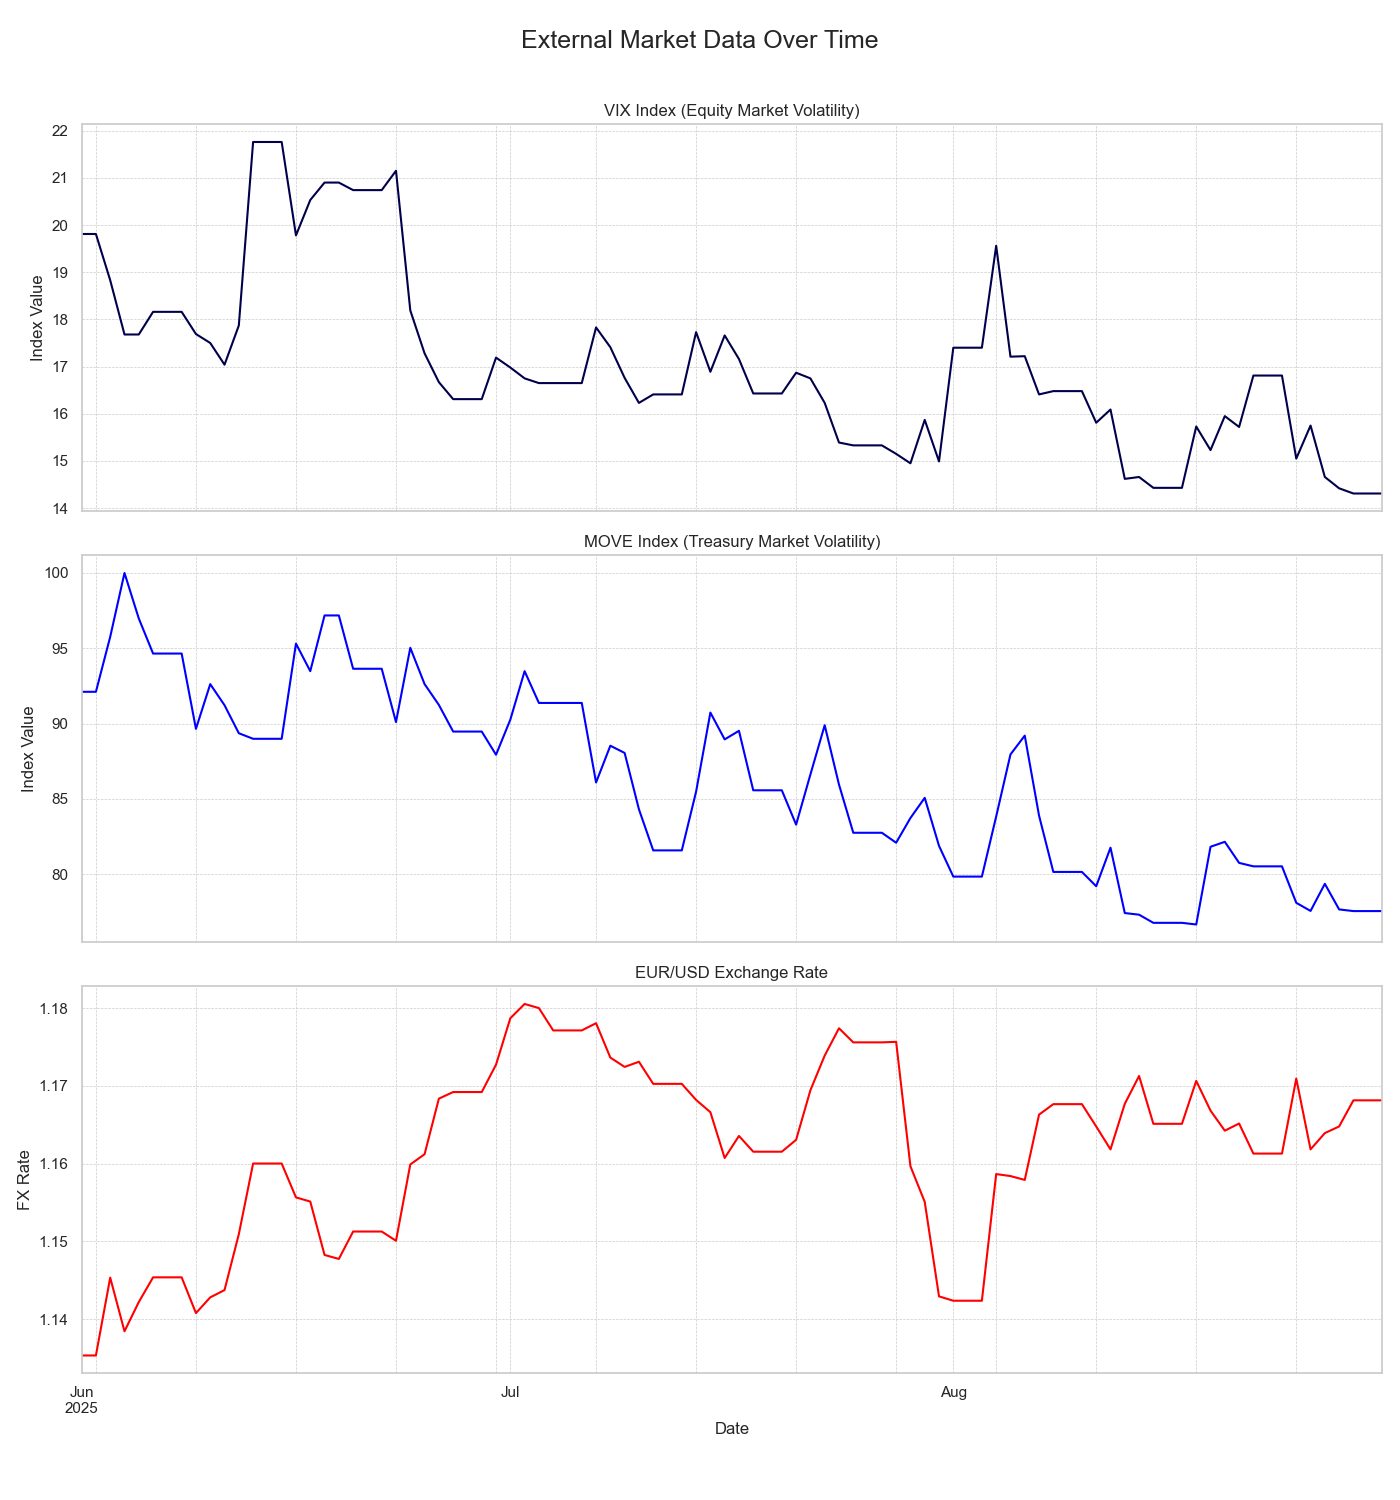
\includegraphics[width=1\textwidth]{images/descriptive_data_analysis/external_data_time_series.png}
	\caption{Time Series of Market-Wide Indicators (VIX, MOVE, and EUR/USD)}
	\label{fig:external_data_time_series}
\end{figure}

Figure~\ref{fig:external_data_time_series} depicts the evolution of key market indicators between June and late August 2025. The overall market environment during this period is characterized by a notable decrease in volatility across major asset classes. The \textit{VIX Index}, representing equity market volatility, begins near a relatively elevated level of 20 before declining sharply in late June and stabilizing within a range of 14–17. This pattern suggests a reduction in perceived equity market risk. Similarly, the \textit{MOVE Index}, a measure of Treasury market volatility, exhibits an even more pronounced decline—from approximately 100 to below 80—indicating a substantial calming of interest rate expectations. Concurrently, the \textit{EUR/USD} exchange rate shows a strengthening of the Euro against the U.S. Dollar, peaking near 1.18 in mid-July before a modest correction. These co-evolving patterns reflect a broad reduction in cross-asset risk and uncertainty.

% --- TABLE 1 INSERTED HERE ---
\begin{table}[H]
	\centering
	\begin{threeparttable}
		\caption{Summary Statistics of External Market Factors}
		\label{tab:external_summary}
		\begin{tabular}{lccccc}
			\toprule
			\textbf{Factor} & \textbf{Mean} & \textbf{Median} & \textbf{Std. Dev.} & \textbf{Skewness} & \textbf{Kurtosis} \\
			\midrule
			VIX Index       & 17.05         & 16.71           & 1.89               & 0.89              & 0.34              \\
			MOVE Index      & 86.29         & 86.02           & 6.12               & 0.10              & -1.10             \\
			EUR/USD Rate    & 1.162         & 1.164           & 0.011              & -0.57             & -0.54             \\
			\bottomrule
		\end{tabular}
		\begin{tablenotes}
			\footnotesize
			\item  A summary of the key external market factors over the analysis period. The positive skew in the VIX index and the non-zero kurtosis across all factors suggest deviations from a normal distribution.
		\end{tablenotes}
	\end{threeparttable}
\end{table}


Table~\ref{tab:external_summary} provides a quantitative summary of the external market factors depicted in Figure~\ref{fig:external_data_time_series}. The statistics confirm the visual analysis, detailing the central tendency and dispersion of each series. Notably, the VIX Index exhibits significant positive skewness (0.89), indicating that upward spikes in volatility are more pronounced than downward movements. Conversely, the EUR/USD rate shows a negative skew (-0.57). The kurtosis values, which deviate from the zero value of a mesokurtic distribution, provide further numerical evidence that these financial time series are not normally distributed, a crucial consideration for the modeling approach.

\begin{figure}[H]
	\centering
	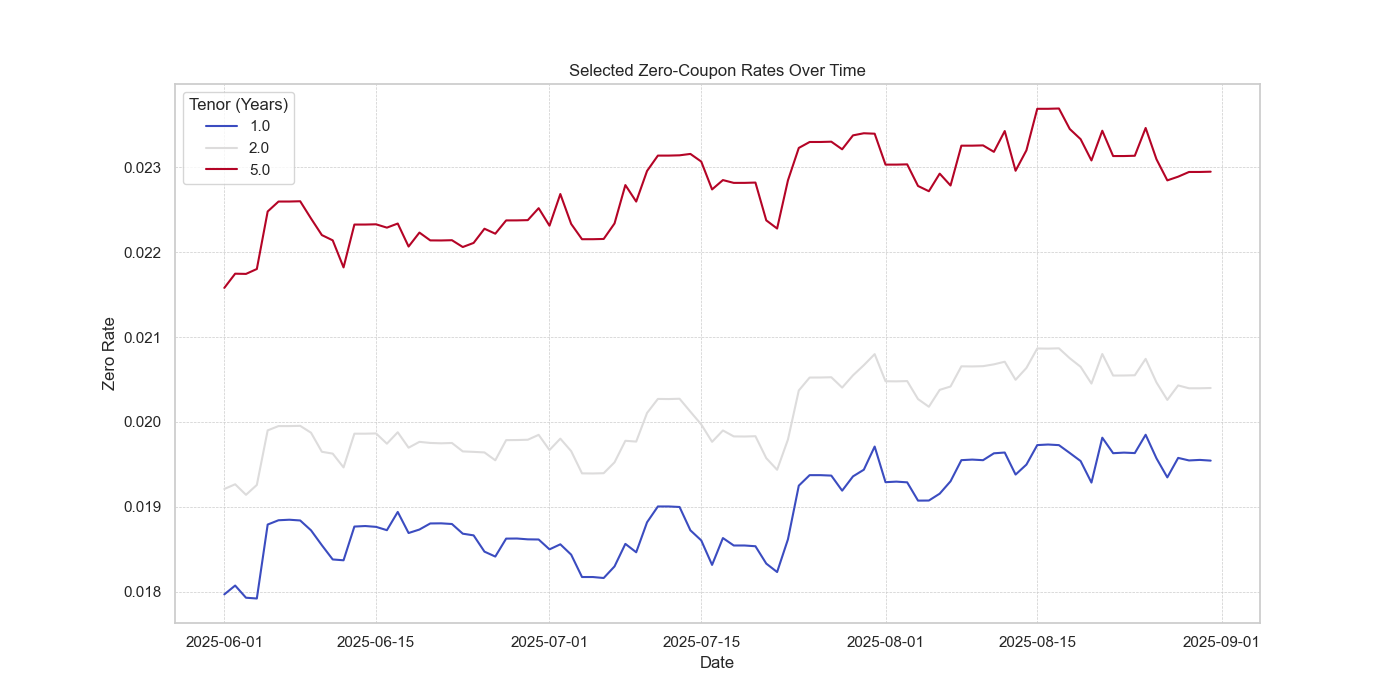
\includegraphics[width=1\textwidth]{images/descriptive_data_analysis/yield_curve_selected_tenors.png}
	\caption{Yield Curve Dynamics for Selected Tenors (1Y, 2Y, 5Y)}
	\label{fig:yield_curve_selected_tenors}
\end{figure}

Figure~\ref{fig:yield_curve_selected_tenors} illustrates the time series of yields across selected maturities. The yield curve retains its normal, upward-sloping shape throughout the observation window. A gradual upward shift is visible across all tenors, indicating a moderate tightening of monetary conditions. The largely parallel movement across maturities implies that changes are predominantly driven by a “level” factor. Minor deviations in spreads, however, suggest that “slope” and “curvature” components contribute modestly to the curve’s dynamics.

\begin{figure}[H]
	\centering
	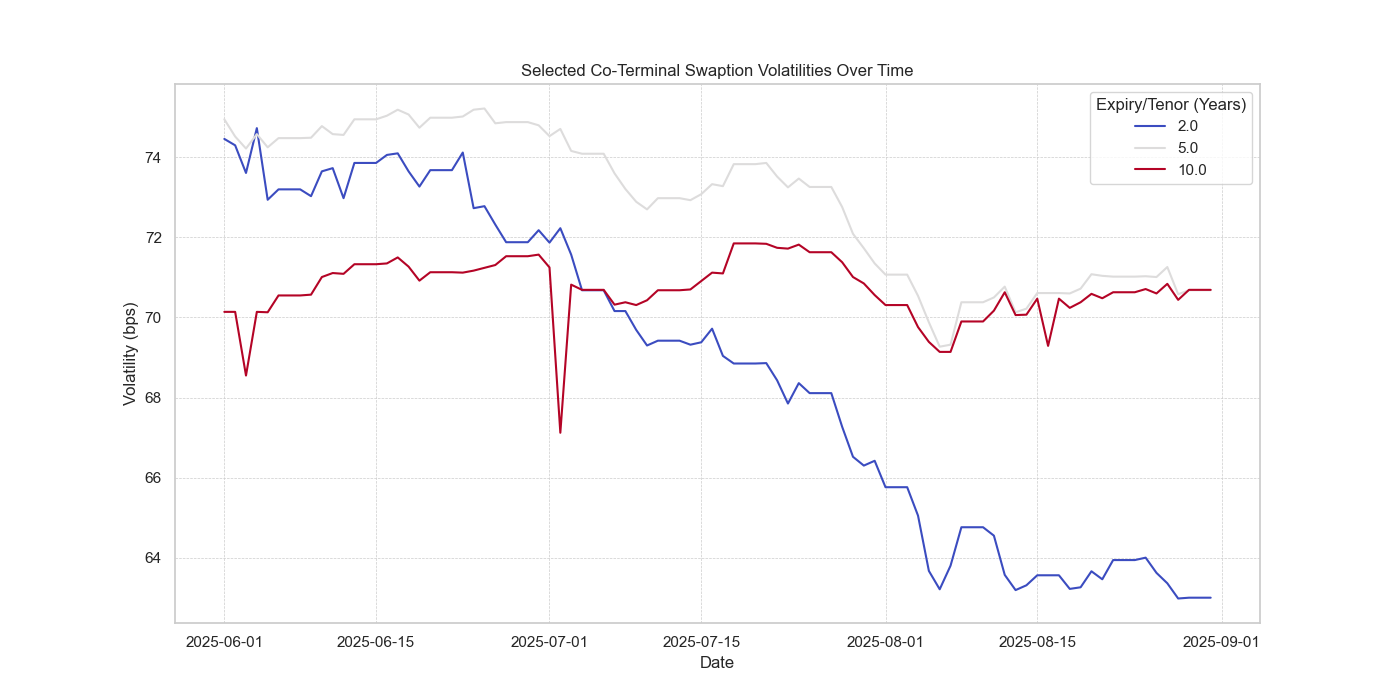
\includegraphics[width=1\textwidth]{images/descriptive_data_analysis/vol_surface_coterminal_series.png}
	\caption{Time Series of Co-Terminal Swaption Volatilities}
	\label{fig:vol_surface_coterminal_series}
\end{figure}

Figure~\ref{fig:vol_surface_coterminal_series} presents the evolution of the co-terminal swaption volatility term structure. The curve is generally downward sloping, with shorter maturities exhibiting higher volatility levels than longer maturities. The short-term (2-year) volatility declines sharply from over 74~bps to approximately 63~bps, whereas the long-term (10-year) volatility remains comparatively stable. This differential behavior leads to a pronounced flattening of the volatility term structure—a key empirical feature that any robust model should accurately capture.

\begin{figure}[H]
	\centering
	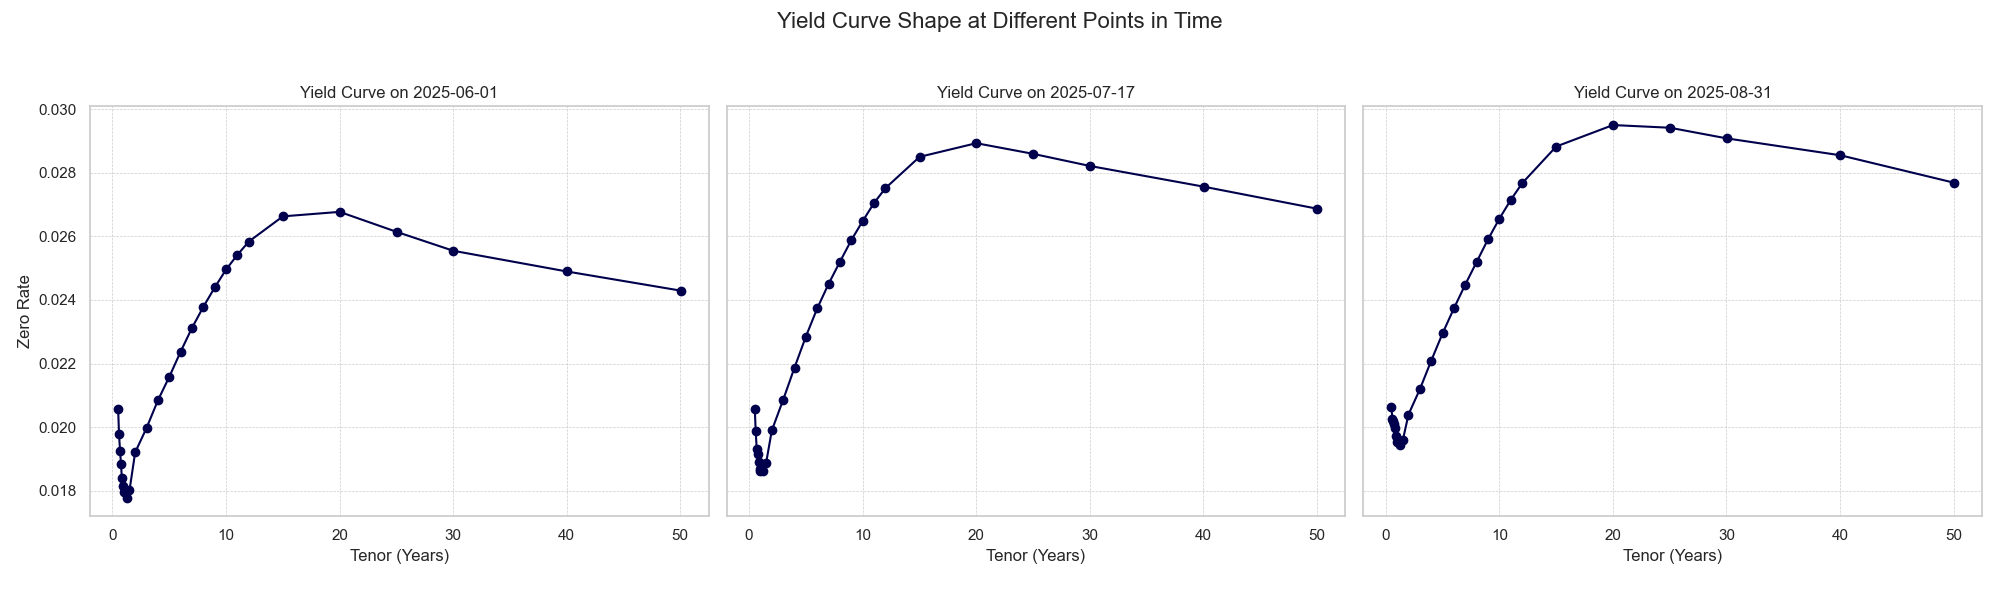
\includegraphics[width=1\textwidth]{images/descriptive_data_analysis/yield_curve_2d_snapshots.png}
	\caption{Yield Curve Snapshots over Time}
	\label{fig:yield_curve_2d_snapshots}
\end{figure}

Figure~\ref{fig:yield_curve_2d_snapshots} visualizes static yield curve snapshots at different points in time. The yield curve consistently displays a concave, upward-sloping shape, typical for stable economic environments. The entire curve shifts upward from June to August, reinforcing the observed trend of rising interest rates. Moreover, the curvature appears to increase slightly over time, suggesting subtle changes in the underlying term structure dynamics.

% --- TABLE 2 INSERTED HERE ---
\begin{table}[H]
	\centering
	\begin{threeparttable}
		\caption{Descriptive Statistics for Key Yield Curve Tenors}
		\label{tab:yield_curve_summary}
		\begin{tabular}{lcccc}
			\toprule
			\textbf{Tenor} & \textbf{Mean Rate (\%)} & \textbf{Std. Dev. (\%)} & \textbf{Skewness} & \textbf{Kurtosis} \\
			\midrule
			1-Year         & 1.90                    & 0.05                    & -0.02             & -1.10             \\
			5-Year         & 2.27                    & 0.05                    & -0.18             & -0.88             \\
			10-Year        & 2.62                    & 0.06                    & -0.25             & -1.04             \\
			30-Year        & 2.76                    & 0.12                    & -0.29             & -1.22             \\
			\bottomrule
		\end{tabular}
		\begin{tablenotes}
			\footnotesize
			\item  Descriptive statistics for selected benchmark tenors of the zero-coupon yield curve. Mean Rate and Standard Deviation are expressed in percentage points.
		\end{tablenotes}
	\end{threeparttable}
\end{table}


Table~\ref{tab:yield_curve_summary} quantifies the characteristics of the yield curve by presenting descriptive statistics for key benchmark tenors. The increasing mean rate with tenor numerically confirms the upward-sloping nature of the term structure. A particularly important finding is the behavior of the standard deviation, which increases from 0.05\% for the 1-year rate to 0.12\% for the 30-year rate. This demonstrates that the long end of the yield curve is substantially more volatile in absolute terms, a stylized fact that is further explored in Figure~\ref{fig:yield_curve_std_by_tenor}.

\begin{figure}[H]
	\centering
	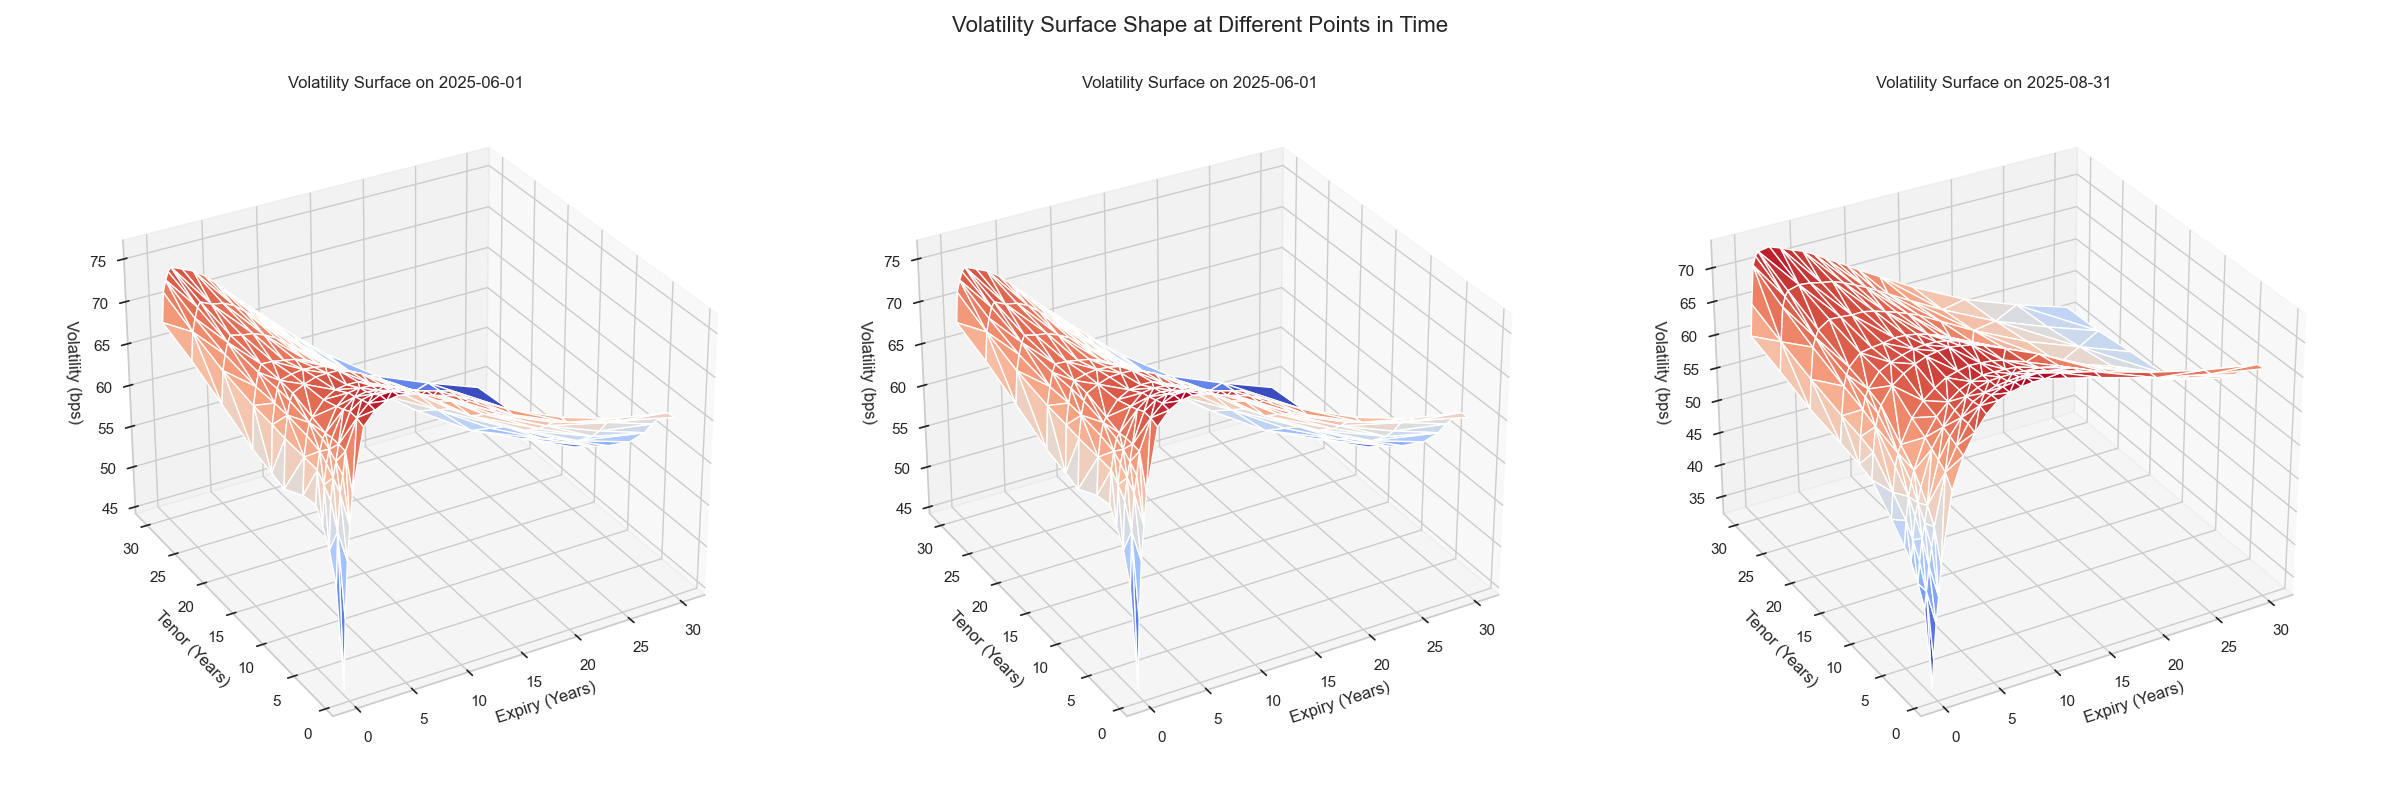
\includegraphics[width=1\textwidth]{images/descriptive_data_analysis/vol_surface_3d_snapshots.png}
	\caption{3D Representation of the Swaption Volatility Surface}
	\label{fig:vol_surface_3d_snapshots}
\end{figure}

Figure~\ref{fig:vol_surface_3d_snapshots} provides a three-dimensional representation of the swaption volatility surface. The surface exhibits pronounced structure, with the highest volatilities concentrated in short-expiry, short-tenor instruments. Volatility decreases along both the expiry and tenor dimensions, forming a characteristic “hump” at the short end. This structural complexity underscores the necessity of employing non-linear modeling approaches—such as neural networks—to accurately capture the surface’s intricate shape and temporal dynamics.

\begin{figure}[H]
	\centering
	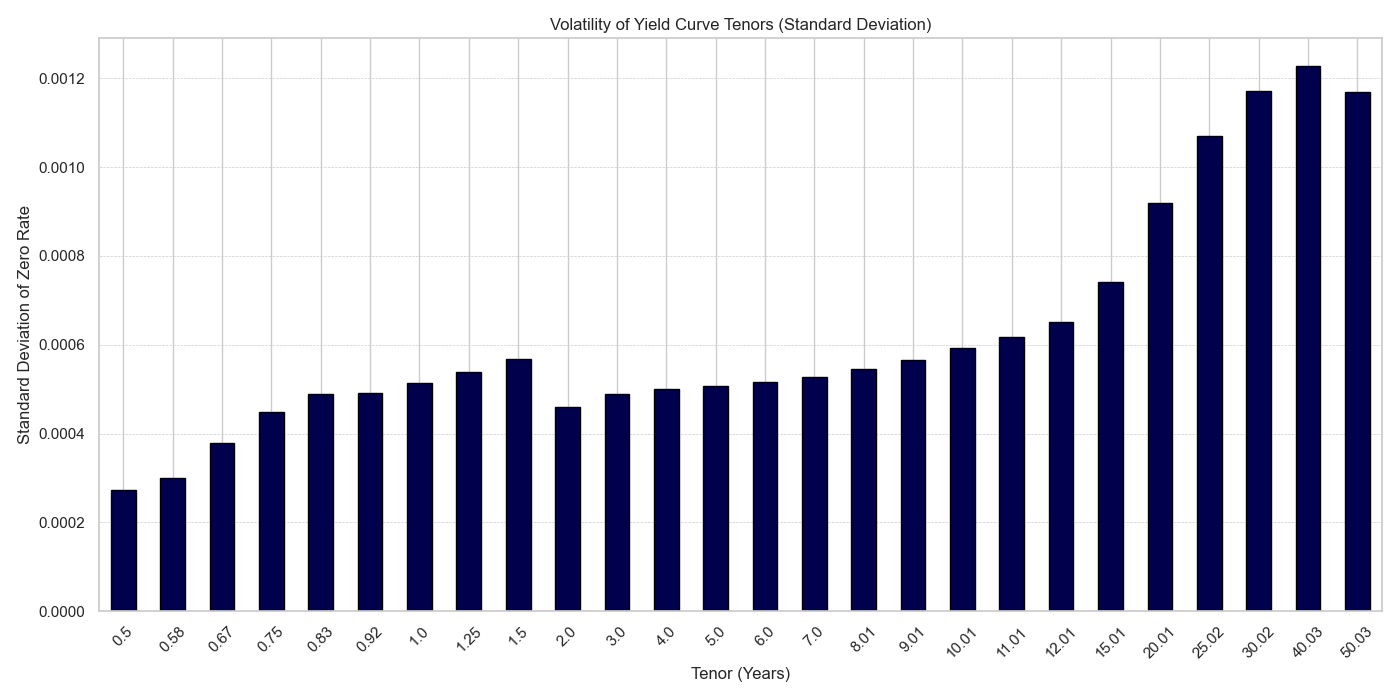
\includegraphics[width=1\textwidth]{images/descriptive_data_analysis/yield_curve_std_by_tenor.png}
	\caption{Standard Deviation of Daily Yield Changes by Tenor}
	\label{fig:yield_curve_std_by_tenor}
\end{figure}

Figure~\ref{fig:yield_curve_std_by_tenor} shows the distribution of yield volatility across maturities. Volatility is lowest at the short end, increases moderately in the 1–2 year range, and rises significantly for longer maturities beyond 10 years. This pattern highlights that long-term yields exhibit the greatest absolute variability, a crucial consideration for risk management and model calibration.

\begin{figure}[H]
	\centering
	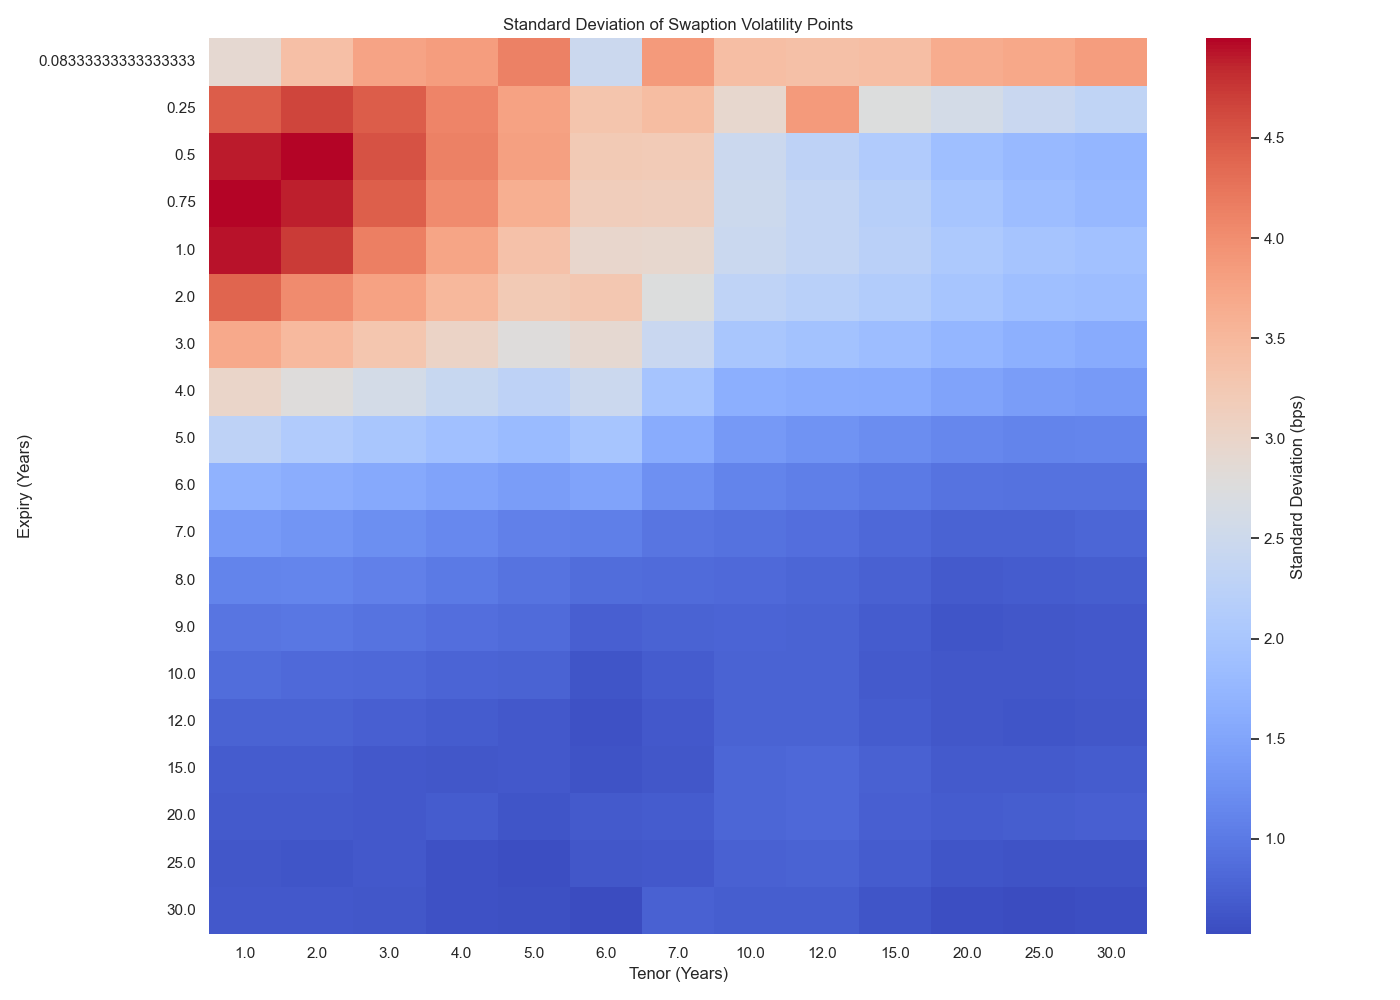
\includegraphics[width=1\textwidth]{images/descriptive_data_analysis/vol_surface_std_heatmap.png}
	\caption{Heatmap of Swaption Volatility Surface Standard Deviations}
	\label{fig:vol_surface_std_heatmap}
\end{figure}

Figure~\ref{fig:vol_surface_std_heatmap} displays the standard deviation of swaption volatilities across expiry and tenor dimensions. The highest volatility—represented by the most intense red shading—is concentrated in the short-expiry, short-tenor region. This indicates that the front end of the surface is particularly unstable, while the long end remains relatively static. A well-performing model must therefore excel at capturing the pronounced temporal variability in this region.

% --- TABLE 3 INSERTED HERE ---
\begin{table}[H]
	\centering
	\begin{threeparttable}
		\caption{Standard Deviation of Swaption Volatilities (in basis points)}
		\label{tab:vol_std_summary}
		\begin{tabular}{lcccc}
			\toprule
			\textbf{Expiry} & \textbf{1-Year Tenor} & \textbf{5-Year Tenor} & \textbf{10-Year Tenor} & \textbf{30-Year Tenor} \\
			\midrule
			1-Year          & 4.93                  & 3.37                  & 2.45                   & 1.92                   \\
			5-Year          & 2.28                  & 1.82                  & 1.35                   & 1.12                   \\
			10-Year         & 0.86                  & 0.75                  & 0.76                   & 0.65                   \\
			30-Year         & 0.66                  & 0.56                  & 0.71                   & 0.54                   \\
			\bottomrule
		\end{tabular}
		\begin{tablenotes}
			\footnotesize
			\item  Standard deviation of daily swaption volatilities, measured in basis points (bps). The table shows the absolute volatility for key points on the expiry-tenor grid.
		\end{tablenotes}
	\end{threeparttable}
\end{table}


Table~\ref{tab:vol_std_summary} provides a quantitative counterpart to the heatmap in Figure~\ref{fig:vol_surface_std_heatmap}, detailing the magnitude of instability across the volatility surface. The data confirms that the highest volatility is located at the front end, with the 1-year expiry, 1-year tenor swaption exhibiting a standard deviation of 4.93 bps. This value is nearly an order of magnitude larger than the 0.54 bps standard deviation observed for the 30-year expiry, 30-year tenor swaption. This sharp gradient in instability underscores the modeling challenge: the neural network must learn to produce highly dynamic outputs for the front end of the surface while generating stable outputs for the back end.

\begin{figure}[H]
	\centering
	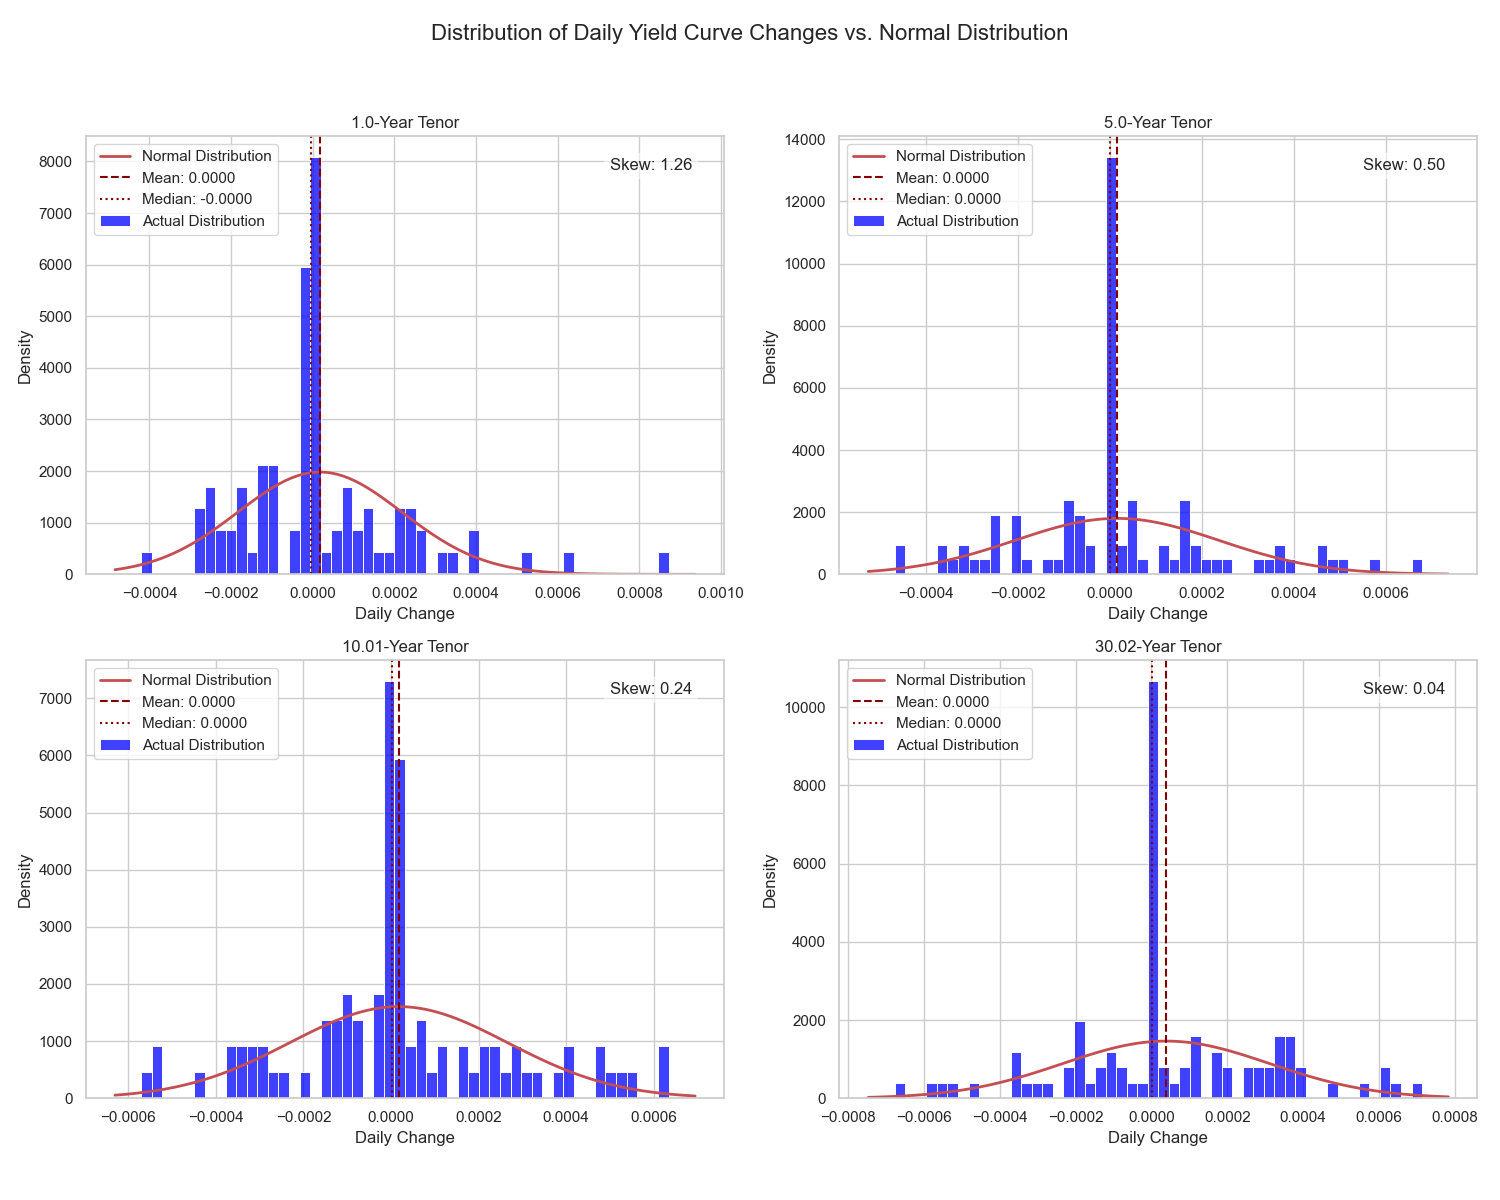
\includegraphics[width=1\textwidth]{images/descriptive_data_analysis/yield_curve_daily_changes_histogram.png}
	\caption{Histograms of Daily Yield Changes by Tenor}
	\label{fig:yield_curve_daily_changes_histogram}
\end{figure}

Figure~\ref{fig:yield_curve_daily_changes_histogram} compares empirical histograms of daily interest rate changes with theoretical normal distributions. All tenors display leptokurtic distributions with fat tails, implying that extreme movements occur more frequently than predicted by Gaussian models. The 1-year tenor exhibits pronounced positive skewness (1.26), suggesting a tendency toward larger upward rate movements. Skewness gradually declines for longer maturities. These findings confirm that interest rate changes deviate substantially from normality.

\begin{figure}[H]
	\centering
	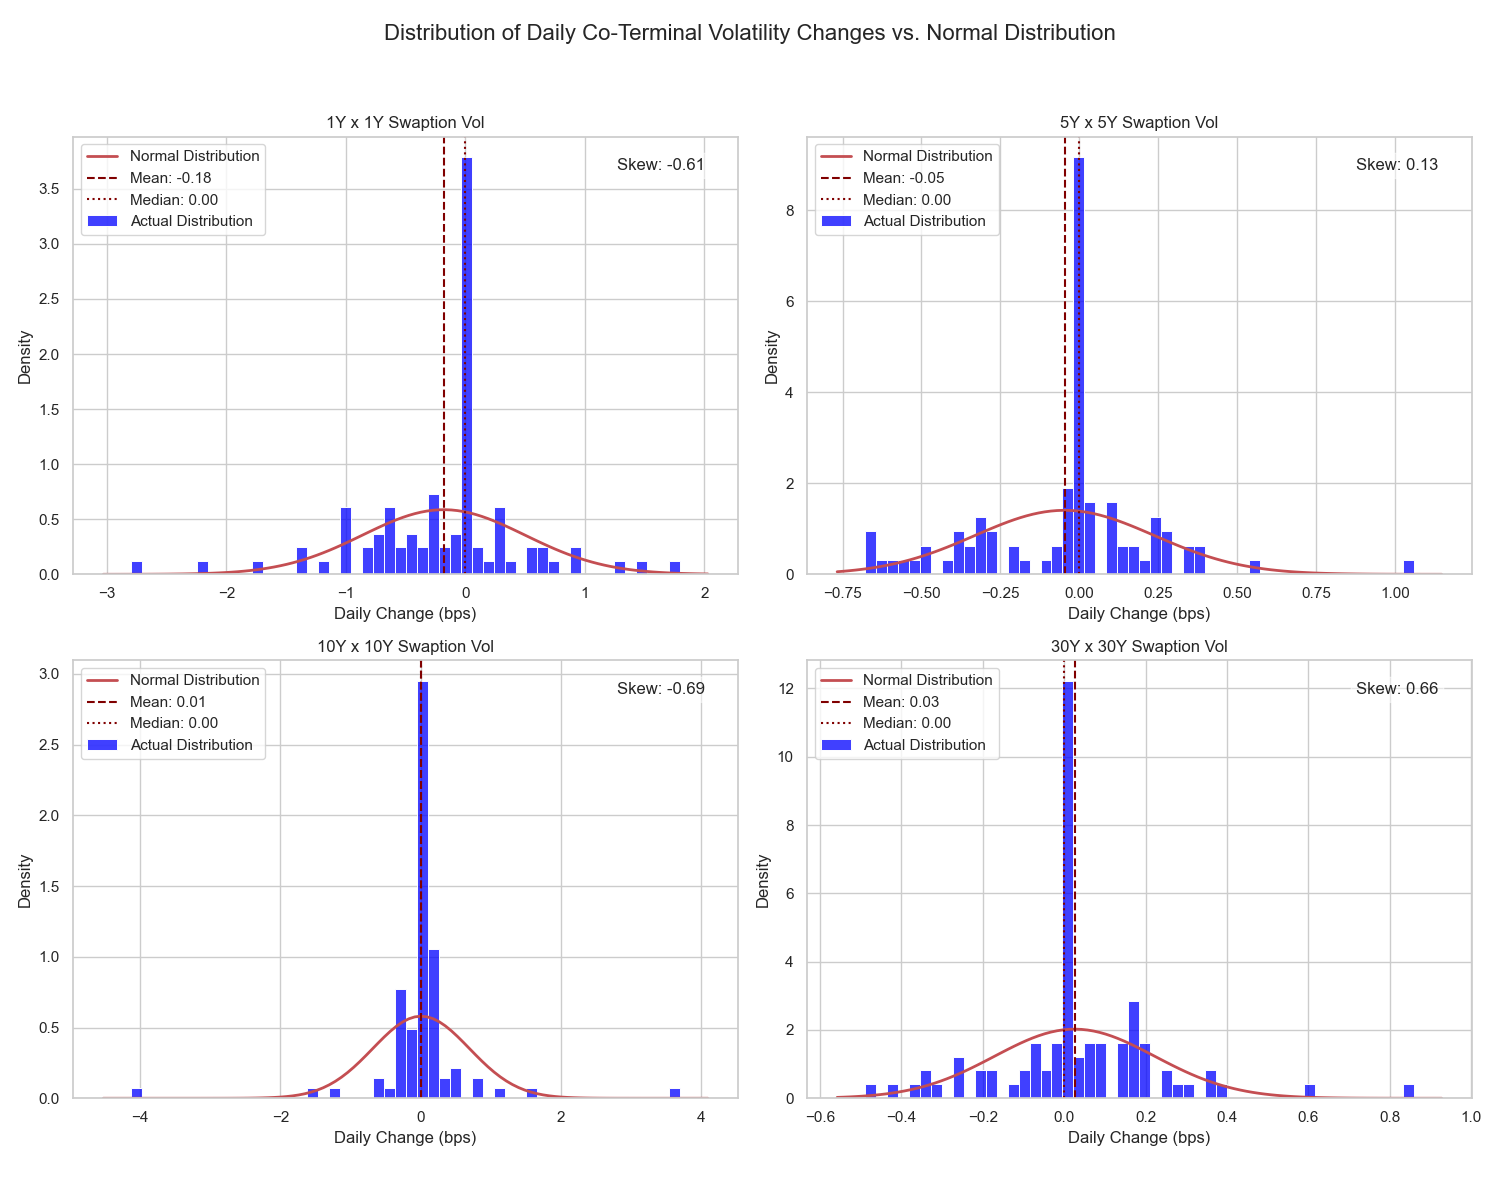
\includegraphics[width=1\textwidth]{images/descriptive_data_analysis/vol_surface_daily_changes_histogram.png}
	\caption{Histograms of Daily Swaption Volatility Changes}
	\label{fig:vol_surface_daily_changes_histogram}
\end{figure}

Figure~\ref{fig:vol_surface_daily_changes_histogram} presents the distribution of daily changes in swaption volatilities. Similar to yield changes, the data exhibit significant leptokurtosis and fat tails, confirming the non-normal nature of the underlying process. A mild positive skew is particularly evident in the 5-year tenor (skew = 0.50), indicating that large volatility spikes are more frequent than declines. Together with the findings from Figure~\ref{fig:yield_curve_daily_changes_histogram}, this evidence supports the use of non-parametric, data-driven models—such as neural networks—that can flexibly capture these empirical deviations from normality.

\subsection{Data Preprocessing}
\subsubsection{Bootstrapping Zero-Curves}
The implementation of the one-factor Hull–White model in \texttt{QuantLib} requires zero-coupon curves as input for both discounting and forward-rate generation. Consequently, the EUR swap curves obtained from Bloomberg were bootstrapped into continuous zero-rate term structures following the procedure outlined in subsection~\ref{subsec:bootstrap_zero_curve}. This ensures compatibility with the \texttt{QuantLib} framework and provides a consistent foundation for pricing swaptions and calibrating the model parameters.

\subsubsection{Handling Non-Trading Days in External Data}
The external market data obtained from Yahoo Finance, including the MOVE index, VIX index, and EUR/USD exchange rate, is only available for trading days. In contrast, the swaption and swap curve datasets contain values for all calendar days, including weekends and public holidays. To ensure temporal consistency across all features used for Hull–White model calibration, the external data were reindexed to cover the entire daily date range of the analysis period.

Missing values corresponding to non-trading days were filled using a combination of forward-filling and {backward-filling. Forward-filling propagates the most recent available value to subsequent missing days, while backward-filling assigns the nearest subsequent available value to preceding missing days. This procedure ensures that every day within the observation window has a corresponding value for each external variable, resulting in a continuous dataset that can be used by the neural network without introducing gaps or inconsistencies.

\subsubsection{Feature Engineering for the Neural Network}
In addition to the raw market data, several engineered features were created to enhance the neural network's ability to predict Hull–White model parameters. These features capture the shape of the yield curve, relationships between external market indicators, and underlying latent structures via dimensionality reduction. Each feature was designed with a clear economic or statistical justification for its relevance to the model parameters: the volatility \(\sigma\) and the mean-reversion speed \(a\).

\paragraph{Features Engineered from the Yield Curve}
These features explicitly describe the shape and dynamics of the zero-coupon interest rate term structure. Let \(\text{Rate}(T)\) denote the zero-coupon rate for a given tenor \(T\) (e.g., \(\text{Rate}(10\text{Y})\) is the 10-year rate).

\textit{Slope Features:}
\begin{equation}
	\text{slope\_3m10y} = \text{Rate}(10\text{Y}) - \text{Rate}(3\text{M})
\end{equation}

\begin{equation}
	\text{slope\_2y10y} = \text{Rate}(10\text{Y}) - \text{Rate}(2\text{Y})
\end{equation}

\begin{equation}
	\text{slope\_5y30y} = \text{Rate}(30\text{Y}) - \text{Rate}(5\text{Y})
\end{equation}

A steep positive slope typically signals expectations of economic growth and future rate hikes, implying higher expected interest rate volatility (\(\sigma\)). Conversely, a flat or inverted curve suggests a more stable rate environment and lower \(\sigma\). Regarding mean reversion (\(a\)), a steep curve indicates strong anchoring to the long-term average, implying higher \(a\), while an inverted curve signals weaker anchoring and lower \(a\).

\textit{Curvature Features:}
\begin{equation}
	\text{curvature\_2y5y10y} = 2 \cdot \text{Rate}(5\text{Y}) - \text{Rate}(2\text{Y}) - \text{Rate}(10\text{Y})
\end{equation}

\begin{equation}
	\text{curvature\_1y2y5y} = 2 \cdot \text{Rate}(2\text{Y}) - \text{Rate}(1\text{Y}) - \text{Rate}(5\text{Y})
\end{equation}

\begin{equation}
	\text{curvature\_10y20y30y} = 2 \cdot \text{Rate}(20\text{Y}) - \text{Rate}(10\text{Y}) - \text{Rate}(30\text{Y})
\end{equation}

High curvature indicates significant uncertainty in medium-term rates, aiding prediction of the term structure of \(\sigma\). Pronounced curvature suggests rates are expected to revert to a mean, implying higher \(a\). Flat curvature indicates weaker mean reversion and lower \(a\).

\paragraph{Features Engineered from External Market Data} \mbox{}\\
\textit{Curvature-to-Slope Ratio:}
\begin{equation}
	\text{curvature\_slope\_ratio} = \frac{\text{curvature\_2y5y10y}}{\text{slope\_2y10y}}
\end{equation}
This feature captures nuanced market regimes where slope and curvature provide complementary information. It allows the network to distinguish between different economic environments and predict both \(\sigma\) and \(a\) more accurately.

\textit{MOVE-to-VIX Ratio:}
\begin{equation}
	\text{MOVE\_VIX\_Ratio} = \frac{\text{MOVE\_Open}}{\text{VIX\_Open}}
\end{equation}
A high ratio indicates stress concentrated in the bond market, signaling a higher \(\sigma\) specific to interest rates. It also implies uncertainty about central bank policy, potentially reducing \(a\). This feature helps the network separate general market panics from fixed-income-specific volatility.

\paragraph{Features Engineered via Dimensionality Reduction}
Instead of feeding all individual zero-coupon rates directly into the neural network, the yield curve was transformed using Principal Component Analysis (PCA). The reason for this choice lies in the fact that individual rates on the curve are highly correlated — a move in the 5-year rate is almost always accompanied by similar movements in the 7-year and 10-year rates as visible in figure \ref{fig:feature_correlation_prePCA}. Using these raw, correlated rates introduces several problems: multicollinearity, redundant information, and an increased risk of overfitting.

\begin{figure}[H]
	\centering
	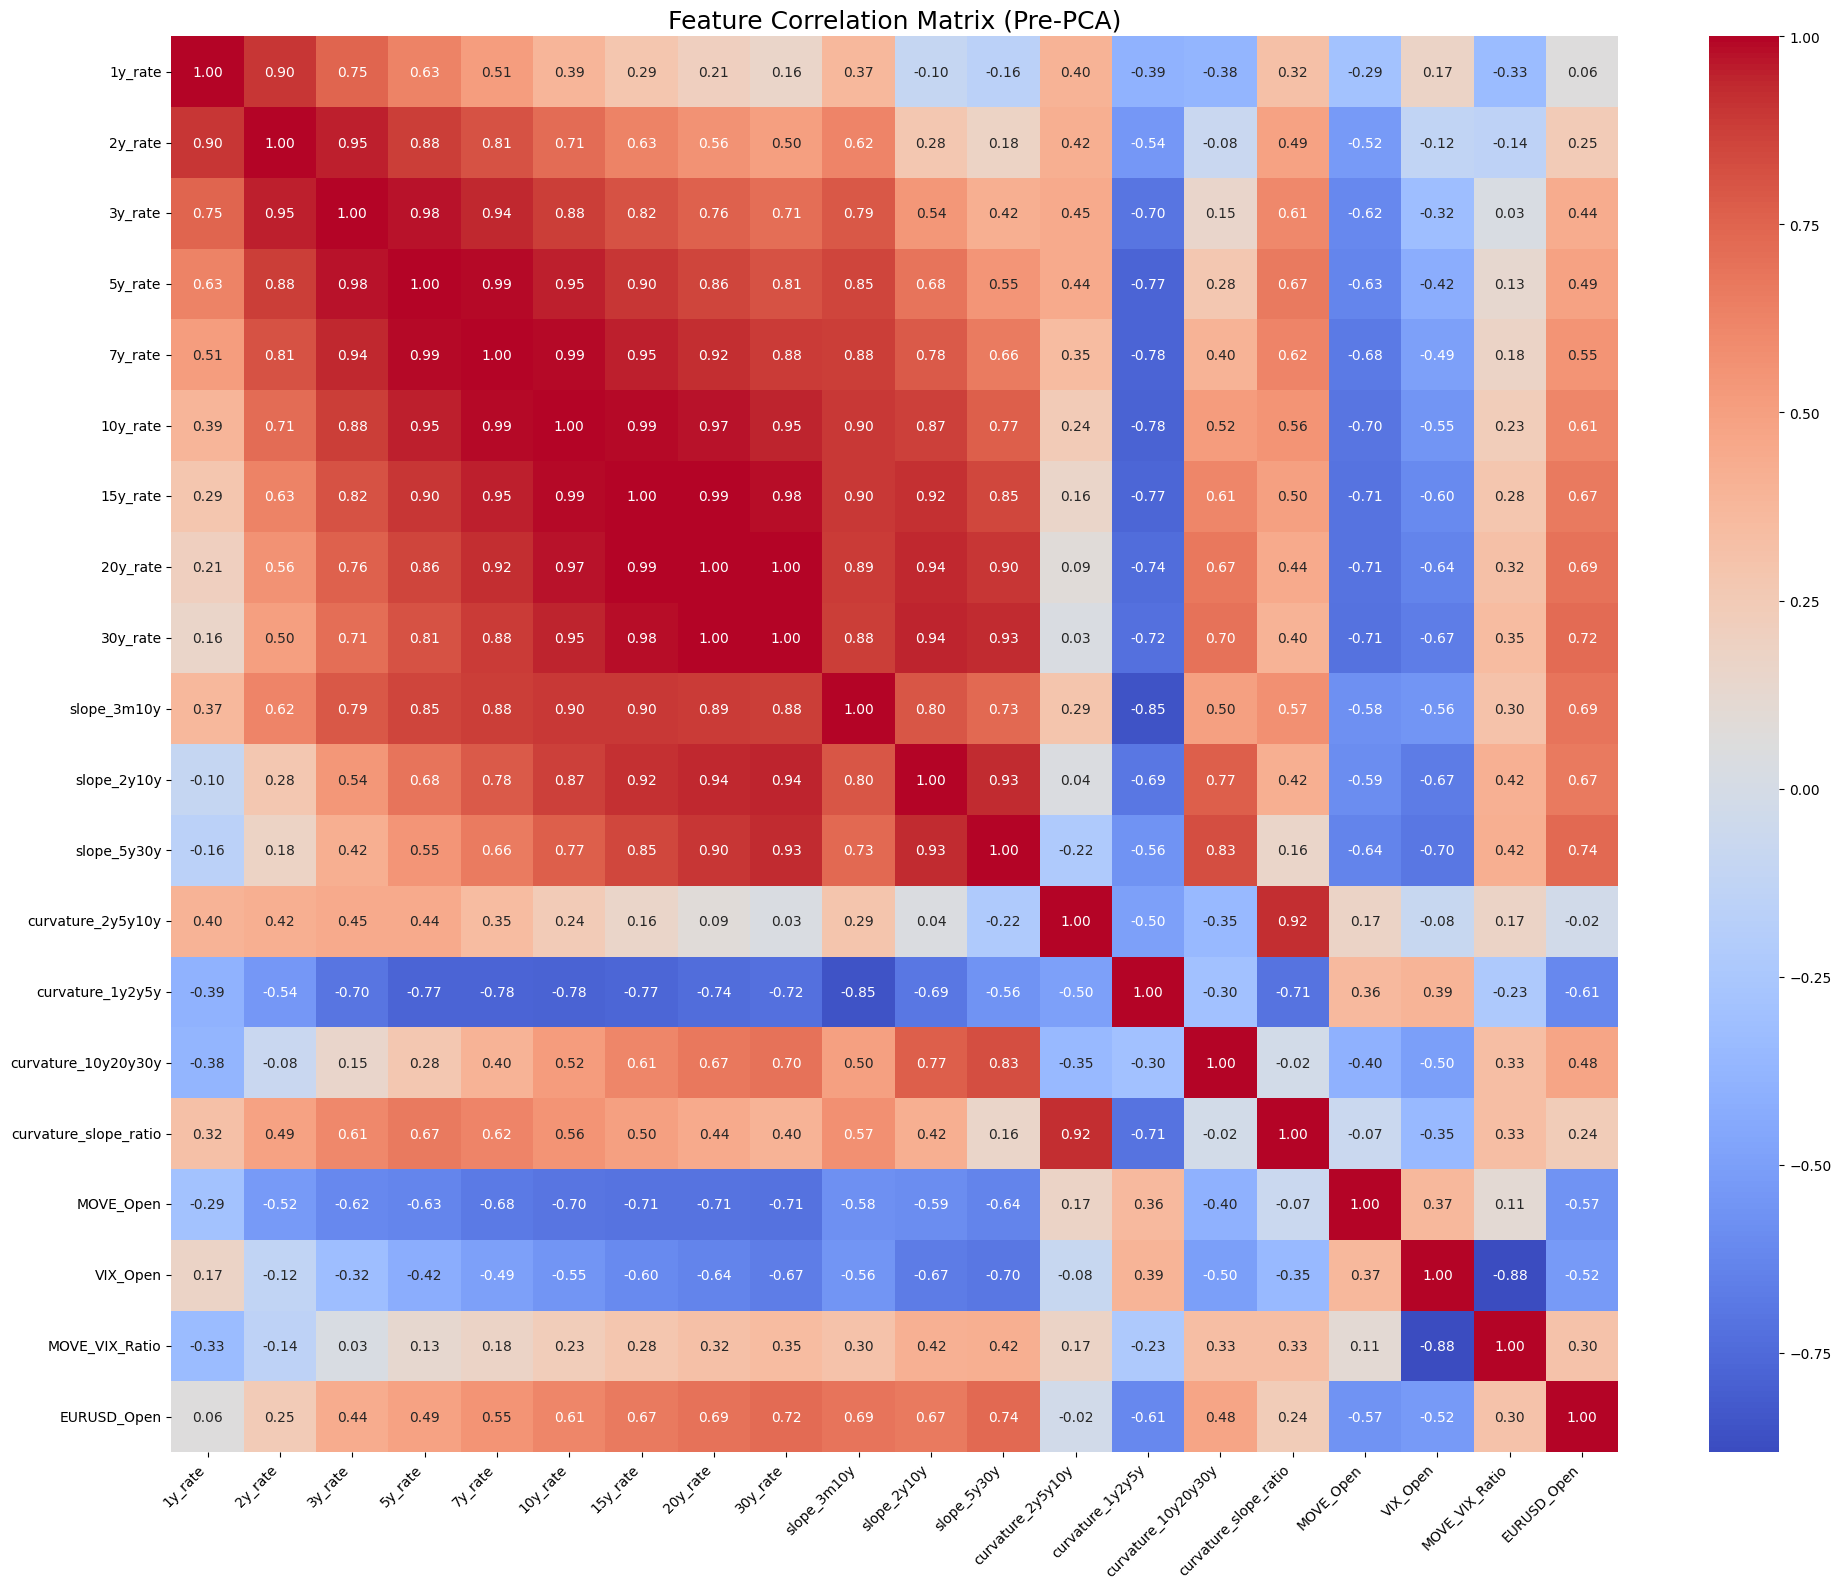
\includegraphics[width=1\textwidth]{images/features/feature_correlation_matrixPre-PCA.png}
	\caption{Correlation matrix of the engineered features before applying PCA.}
	\label{fig:feature_correlation_prePCA}
\end{figure}

Multicollinearity causes instability in the learned weights of the neural network. When input features contain overlapping information, the model struggles to assign stable importance to each feature. It may assign large, offsetting weights to features that move together, resulting in unstable and unreliable predictions \parencite[p.~2]{chan2022multicollinearity}.

Redundant information makes the learning process inefficient and typically leads to poor test performance \parencite[p.~3]{sildir2020redudantfeatures}. Most daily movements in the yield curve are dominated by a single pattern — a parallel shift. Feeding the model all the raw rates forces it to re-learn this shared structure repeatedly instead of focusing on economically meaningful dynamics such as slope or curvature changes.

High dimensionality further increases the complexity of the model, encouraging overfitting. With too many correlated features, the neural network risks memorizing noise instead of generalizable relationships, which harms out-of-sample performance \parencite[p.~3]{sildir2020redudantfeatures}.

PCA directly resolves these issues by transforming the vector of rates
\[
	R = [\text{Rate}(1\text{Y}), \text{Rate}(2\text{Y}), \dots, \text{Rate}(30\text{Y})]
\]
into a set of uncorrelated and economically interpretable components:
\begin{equation}
	\text{PC\_Level} = \mathbf{w}_1 \cdot \mathbf{R}
\end{equation}
\begin{equation}
	\text{PC\_Slope} = \mathbf{w}_2 \cdot \mathbf{R}
\end{equation}
\begin{equation}
	\text{PC\_Curvature} = \mathbf{w}_3 \cdot \mathbf{R}
\end{equation}

These three “super-features” capture nearly all the meaningful variation of the yield curve and can be interpreted as follows \parencite[pp.~98--107]{Rebonato_2018}:
\begin{itemize}
	\item PC\_Level represents the overall interest rate level and captures parallel shifts. Empirically, higher rate levels are associated with higher volatility (\(\sigma\)).
	\item PC\_Slope measures the steepness of the curve and reflects economic expectations, influencing both \(\sigma\) and \(a\).
	\item PC\_Curvature captures the non-linear “bow” of the curve, aiding the model in learning term-structure effects in the piecewise $\sigma$ and mean-reversion dynamics $\alpha$.
\end{itemize}

After applying PCA to the engineered features, the resulting correlation matrix exhibits a significant reduction in the highest correlations. The originally strong dependencies between individual yield curve rates and other features are largely removed as visible in figure \ref{fig:feature_correlation_postPCA}, demonstrating that the principal components provide a set of largely uncorrelated, independent features for the neural network.

\begin{figure}[H]
	\centering
	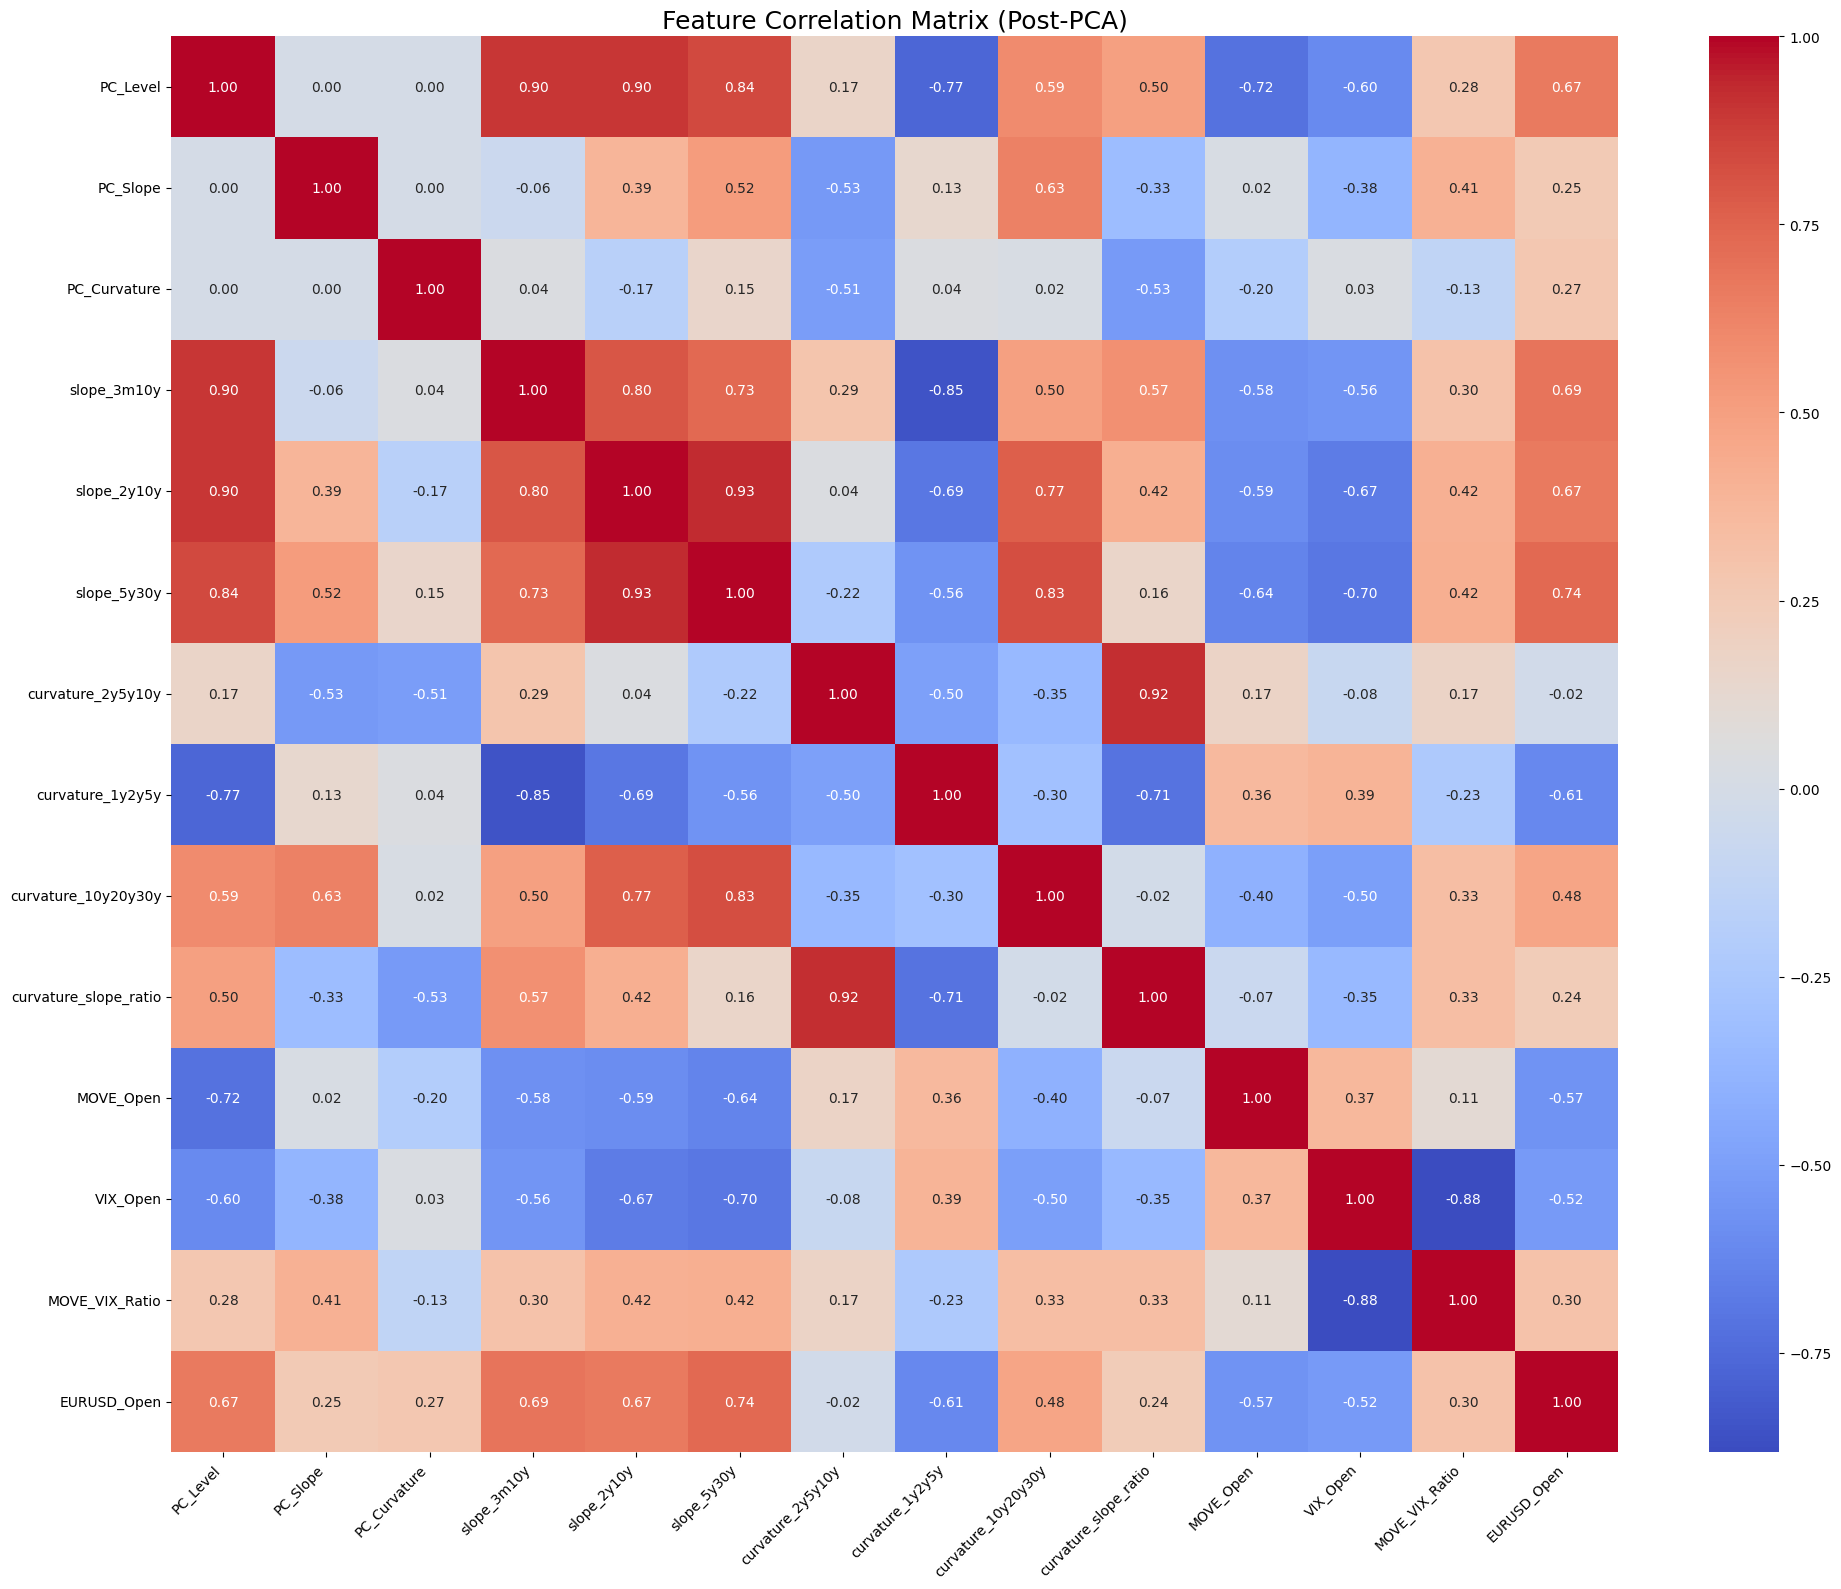
\includegraphics[width=1\textwidth]{images/features/feature_correlation_matrixPost-PCA.png}
	\caption{Correlation matrix of the engineered features after applying PCA.}
	\label{fig:feature_correlation_postPCA}
\end{figure}

By reducing the dimensionality from roughly ten correlated rate inputs to three independent components, PCA provides a stable, interpretable, and compact representation of the yield curve. This significantly improves the neural network’s training efficiency, robustness, and generalization performance.

\subsubsection{Feature Scaling}
Prior to being fed into the neural network, all input features are scaled using the \texttt{StandardScaler} from the \texttt{scikit-learn} library. This process, also known as standardization or Z-score normalization, ensures that each feature has a mean of zero and a standard deviation of one \parencite[pp.~31--32]{zheng2018feature}.

The scaling process consists of two main steps:

\textit{Step 1: Fit Phase (Learning from Training Data)}
The scaler analyzes the training data to learn the distribution of each feature. For each feature column, it calculates:

\begin{equation}
	\mu = \frac{1}{n} \sum_{i=1}^{n} x_i
\end{equation}
\begin{equation}
	\sigma = \sqrt{\frac{1}{n} \sum_{i=1}^{n} (x_i - \mu)^2}
\end{equation}

where \(x_i\) are the individual values of the feature and \(n\) is the number of training samples. The computed mean \(\mu\) and standard deviation \(\sigma\) are stored in the scaler object.

\textit{Step 2: Transform Phase (Applying the Scaling)}
The learned parameters are used to transform all values of that feature in the training, validation, and test datasets:

\begin{equation}
	z = \frac{x - \mu}{\sigma}
\end{equation}

This centers the data around zero and scales it to unit variance.

From a computational perspective, normalization is necessary to manage issues arising from the inherent structure of raw data inputs. It is a technique widely used in statistics for making the units of variables comparable, which is critical when input data are expressed in very different units and exhibit disparate orders of magnitude. Without scaling, features with very large numerical values can dominate the error calculation, causing the error reduction algorithm to focus primarily on these variables while neglecting the information contained in smaller-valued features. Furthermore, when raw numerical values are extremely large, such as on the order of $10^{6}$, their processing can generate outputs that exceed the capacity of standard computing hardware, making scaling essential to control for calculation and roundoff errors \parencite{shanker1996effectdatastandardization}.

The application of scaling directly addresses the optimization landscape of the training problem, leading to more efficient convergence. Normalizing the input is known to accelerate convergence during the optimization of linear models. Linear scale transformations, especially those that compress the search space, reduce the distance the backpropagation algorithm must cover in each iteration \parencite{sola1997importancedatanormalization}. This improved conditioning, where normalization helps ensure the covariance matrix of the layer input $\sum{}x$ is well-conditioned, is crucial for faster learning and aids the optimization algorithm in locating local minima \parencite{huang2020normalizationtechniquestrainingdnns}. Consequently, an adequate normalization protocol can significantly reduce calculation and training time, with studies showing that estimation errors can be reduced by a factor of 5 to 10 and the time required to achieve such results reduced by an order of magnitude \parencite{sola1997importancedatanormalization}.

Ultimately, the primary result of standardization is an improvement in the neural network's quality and training stability. Data transformation is frequently used for improved learning, and normalization techniques are considered essential for accelerating the training and enhancing the generalization of deep neural networks (DNNs). Networks trained on standardized data generally yield better overall results, leading to a higher classification rate and a smaller Mean Square Error (MSE) in regression problems, where a smaller MSE indicates a higher quality solution \parencite{shanker1996effectdatastandardization}. The performance of a network, including the number of training iterations required and the final error attained, is enhanced as the input variable ranges are 'equalized' by the normalization process. This contributes to scale-invariant learning, which is important for stabilizing training and has been shown to be useful for adaptively adjusting the learning rate. In some cases, standardization is not merely a best practice but a formal prerequisite due to specific algorithm requirements \parencite{huang2020normalizationtechniquestrainingdnns}.

By applying \texttt{StandardScaler}, the neural network receives a well-conditioned, standardized input, which improves training stability, and convergence speed of the resulting model.

\subsection{Hyperparameter Optimization}
\label{subsec:hyperparameter_optimization}

The predictive performance and stability of neural networks depend critically on an appropriate choice of hyperparameters. To identify an optimal configuration, a structured hyperparameter optimization process was conducted using the Hyperband algorithm, as described in Subsection~\ref{subsec:hyperband_algorithm}. This algorithm efficiently allocates computational resources to explore a broad hyperparameter space while focusing on the most promising configurations.

The core settings for the Hyperband tuner were configured as follows:
\begin{itemize}
	\item Maximum Epochs per Trial (\texttt{max\_epochs}): A total of 1000 epochs were allocated as the maximum budget for training any single hyperparameter configuration.
	\item Reduction Factor (\texttt{factor}): A factor of 3 was used, meaning that after each round of training within a bracket, the number of configurations is reduced by a factor of 3, retaining only the top-performing third.
	\item Objective: The optimization objective was the minimization of the root mean squared error on the validation set.
\end{itemize}

The hyperparameters tuned in this study can be divided into two categories: those defining the neural network architecture and those related to the training process and loss function. Hyperparameters related to the architecture are:
\begin{itemize}
	\item Number of Hidden Layers: This parameter determines the depth of the neural network. A deeper network has greater representational power and can capture more complex nonlinear relationships in the data, but it also increases the risk of overfitting and computational cost. \newline
	      \textit{Search Space:} Integer between 1 and 5
	\item Number of Neurons per Layer: The width of each hidden layer, determined by the number of neurons, controls the capacity of the model. Larger layers allow for more detailed pattern recognition but can lead to overfitting if excessive. \newline
	      \textit{Search Space:} Integer between 16 and 128, in steps of 16, for each hidden layer
	\item The activation function introduces non-linearity into the network, enabling it to model complex relationships between input features and outputs. \newline
	      \textit{Search Space:} Choice between \texttt{relu} and \texttt{tanh}.
	\item Dropout is a regularization technique that randomly deactivates a fraction of neurons during training to prevent overfitting by discouraging co-adaptation among neurons. \newline
	      \textit{Search Space:} Boolean choice between \texttt{True} and \texttt{False}.
	\item Dropout Rate: If dropout is used, this parameter determines the fraction of neurons dropped during each training iteration. \newline
	      \textit{Search Space:} Floating-point value between 0.1 and 0.5 (only active if \texttt{use\_dropout = True}) in steps of 0.1.

\end{itemize}

Tuneable hyperparameters which cover the training and the loss functions are:
\begin{itemize}
	\item Learning Rate: The learning rate governs the step size used by the optimizer when updating the model’s weights. A high learning rate may lead to instability or divergence, whereas a very low one results in slow convergence. To capture effective values across orders of magnitude, the search was conducted on a logarithmic scale. \newline
	      \textit{Search Space:} Floating-point value between 0.0001 and 0.01, sampled logarithmically.

	\item Underestimation Penalty: This custom hyperparameter is designed to address the asymmetric cost of forecasting errors in financial volatility modeling. Underestimating volatility poses a greater financial risk than overestimating it. Therefore, this penalty increases the loss when the model underpredicts volatility, encouraging more conservative estimates. \newline
	      \textit{Search Space:} Floating-point value between 0.5 (penalty for overestimation) and 4.0 (strong penalty) in steps of 0.1.
\end{itemize}

\subsection{Loss Function and Error Metric}

The objective of the neural network is to determine the optimal set of weights W and biases b such that the predicted Hull--White parameters minimize the discrepancy between model-implied swaption volatilities and their market-observed counterparts. The neural network acts as a function
\begin{equation}
	\text{NN} : x \mapsto \theta(x; W, b),
\end{equation}
where $x \in \mathbb{R}^d$ is the input feature vector containing scaled and PCA-transformed market data (yield curve levels, slopes, curvatures, etc.) for a given day, and $\theta$ denotes the vector of Hull--White model parameters to be predicted. The network employs a residual architecture: instead of predicting $\theta$ directly, it predicts a deviation $\Delta z$ from a fixed initial guess $z_0$:
\begin{equation}
	\Delta z = \text{NN}(x; W, b), \quad
	z = z_0 + \Delta z.
\end{equation}
The predicted parameters are obtained by applying a scaled sigmoid to ensure they remain within a predefined range [0, U]:
\begin{equation}
	\theta(x; W, b) = U \cdot \sigma(z) = U \cdot \frac{1}{1 + e^{-z}}.
\end{equation}

The predicted parameters $\theta$ are subsequently used within the QuantLib library as a black-box function $V_{\text{QL}}$, which computes model-implied volatilities $\hat{\sigma}$ for a portfolio of $n$ swaptions given the additional market data $M_j$ on day $j$:
\begin{equation}
	\hat{\sigma} = V_{\text{QL}}(\theta, M_j) = \{\hat{\sigma}_1, \hat{\sigma}_2, \dots, \hat{\sigma}_n\}.
\end{equation}

The predictive accuracy of the network is quantified using the root mean squared error (RMSE), which measures the average magnitude of deviation between model-implied and market-observed volatilities, expressed in basis points (bps):
\begin{equation}
	\text{RMSE} = \sqrt{\frac{1}{n}\sum_{i=1}^{n}(\hat{\sigma}_i - \sigma_i)^2} \times 10000.
\end{equation}

\begin{table}[H]
	\centering
	\caption{Notation used in the RMSE formula}
	\begin{tabular}{lp{12cm}}
		\toprule
		Symbol  & Meaning                                                                                                                   \\
		\midrule
		$n$              & Total number of swaptions in the evaluation dataset                                                                                \\
		$\hat{\sigma}_i$ & Implied volatility predicted by the Hull--White model using the parameters generated by the neural network for the $i$-th swaption \\
		$\sigma_i$       & Market-observed implied volatility for the $i$-th swaption                                                                         \\
		\bottomrule
	\end{tabular}
\end{table}

To align the optimization with practical calibration objectives, an asymmetric loss function is employed during training. For each day $j$, the loss is computed as the mean of weighted squared errors between predicted and observed volatilities:
\begin{equation}
	L_j(W, b) = \frac{1}{n} \sum_{i=1}^{n} w_i (\hat{\sigma}_i - \sigma_{j,i})^2,
\end{equation}
where the weight $w_i$ accounts for underestimation penalties:
\begin{equation}
	w_i =
	\begin{cases}
		P, & \text{if } \hat{\sigma}_i < \sigma_{j,i} \quad \text{(underestimation)},   \\
		1, & \text{if } \hat{\sigma}_i \geq \sigma_{j,i} \quad \text{(overestimation)}.
	\end{cases}
\end{equation}
Here, $P>1$ is the underestimation penalty, treated as a hyperparameter optimized using the Hyperband algorithm. This asymmetric weighting is applied exclusively during training to encourage conservative predictions, while evaluation on validation and test sets uses the standard (unweighted) RMSE to assess predictive accuracy objectively.

The overall training objective is to identify network parameters $(W^*, b^*)$ that minimize the expected daily loss over the distribution of training data $D$:
\begin{equation}
	(W^*, b^*) = \arg \min_{W, b} \ \mathbb{E}_{(x_j, \sigma_j, M_j) \sim D} \left[ L_j(W, b) \right].
\end{equation}
In practice, this expectation is approximated by iterating over the training set day by day (batches) using the stochastic optimizer Adam:
\begin{equation}
	W_{t+1} = W_t - \eta \nabla_W L_j(W_t, b_t),
\end{equation}
where $\eta$ is the learning rate. Since $V_{\text{QL}}$ is a non-differentiable black-box function, gradients are computed numerically via finite differences using a tf.custom\_gradient implementation.

\subsection{Methodology Workflow}
The subsequent section delineates the comprehensive, step-by-step workflow implemented for the calibration of the Hull-White model, as depicted by the provided source code. The process is designed as an end-to-end pipeline, commencing with raw data ingestion and culminating in model evaluation, adaptive retraining, and interpretability analysis.

\begin{enumerate}
	\item \textbf{Data Ingestion and Preprocessing:}
	      The initial phase involves loading raw EUR swap curve data, provided in Excel format. For each historical date, the mid-market rate is computed from the bid and ask quotes. These raw swap curves are then processed and transformed into a standardized format. Subsequently, the \texttt{QuantLib} library is employed to bootstrap these swap curves, yielding the corresponding zero-coupon yield curves for each valuation date. This bootstrapping process utilizes a \texttt{PiecewiseLogLinearDiscount} methodology to construct a term structure of zero rates from the observed market swap rates.

	\item \textbf{External Market Data Integration:}
	      To enrich the feature set, external market data is loaded. This includes the ICE BofA MOVE Index (MOVE), which measures US Treasury rate volatility; the CBOE Volatility Index (VIX), which measures equity market volatility; and the EUR/USD foreign exchange rate. This data is sourced via the \texttt{yfinance} library. A complete time series is ensured by forward- and back-filling any missing daily values, providing a consistent set of external features for every yield curve date.

	\item \textbf{Chronological Data Splitting:}
	      Given the time-series nature of the financial data, a strict chronological split is enforced to prevent look-ahead bias. The dataset of available daily yield curves is divided into a training set (the initial 50\%), a validation set (the following 20\%), and a final out-of-sample testing set (the remaining 30\%). This ensures that the model is trained on past data, validated on more recent data, and finally tested on unseen future data.

	\item \textbf{Feature Engineering and Dimensionality Reduction:}
	      For each yield curve, a comprehensive feature vector is engineered. This vector includes not only the zero rates at key tenors (1Y to 30Y) but also derived features such as various yield curve slopes (e.g., 10Y-2Y), curvatures (e.g., $(2 \times 5\text{Y}) - 2\text{Y} - 10\text{Y}$), and the external market indicators. To address the high multicollinearity inherent in yield curve rates, Principal Component Analysis (PCA) is performed exclusively on the rate-based features of the training data. The first three principal components, which typically correspond to the level, slope, and curvature of the yield curve, are retained. This reduces dimensionality while preserving the most significant sources of variance. The complete feature set, comprising these principal components and the other engineered features, is then standardized using Scikit-learn's \texttt{StandardScaler}, which is also fitted solely on the training data.

	\item \textbf{Hyperparameter Optimization:}
	      A rigorous hyperparameter tuning process is conducted using the Hyperband algorithm, implemented via the \texttt{Keras Tuner} library. The search space includes critical model architecture parameters (number of layers, neurons per layer, activation function, dropout usage and rate), optimization parameters (learning rate), and a custom hyperparameter for an asymmetric loss function (underestimation penalty). The objective function for the tuner is the minimization of the root mean squared error (RMSE) on the validation set.

	\item \textbf{Model Training and Early Stopping:}
	      Upon identifying the optimal set of hyperparameters, the final model is retrained from scratch on the entire training set. A key architectural choice is the \texttt{ResidualParameterModel}, which does not predict the Hull-White parameters directly but rather learns a residual correction to a predefined initial guess. Training is performed over a set number of epochs, but an early stopping mechanism is employed. The model's performance on the validation set is monitored after each epoch. If the validation RMSE does not improve for a predefined number of consecutive epochs (patience), the training is halted, and the model weights from the epoch with the lowest validation RMSE are restored. This prevents overfitting to the training data.

	\item \textbf{Out-of-Sample Evaluation and Adaptive Retraining:}
	      The trained model is evaluated on the unseen testing set in a forward-moving, chronological sequence. For each day in the test set, the model predicts the Hull-White parameters, and the resulting calibration error (RMSE) is calculated. This out-of-sample error stream is monitored by the ADWIN (ADaptive WINdowing) algorithm to detect concept drift—a statistically significant degradation in model performance. If ADWIN detects a drift, or if the daily error exceeds a predefined absolute threshold, a retraining event is triggered. In this event, all historical data up to the point of the trigger (original training, validation, and the processed portion of the test set) is used to form a new, larger training set, and the entire workflow from step 4 onwards is repeated. This rolling approach allows the model to adapt to changing market regimes.

	\item \textbf{Model Explainability with SHAP:}
	      To ensure transparency and interpretability of the final trained model, a post-hoc analysis is conducted using SHAP (SHapley Additive exPlanations). A \texttt{DeepExplainer} is utilized to compute SHAP values for the model's predictions on the test set. This analysis quantifies the contribution of each input feature (e.g., PC Level, MOVE Index) to the prediction of each output Hull-White parameter. The results are visualized through summary and feature importance plots, providing crucial insights into the model's decision-making process.
\end{enumerate}

\subsection{Used Model Architecture \& Setup}
\begin{itemize}
	\item Description of how the actual used model is setup, trained and other technical details
	\item Model does not directly predict the parameters of the Hull-White model but predicts the correction of an initial guess e.g. the parameters from the last calibration (for example yesterday) or the parameters determined by the traditional calibration (hybrid approach)
\end{itemize}

\subsection{Calibration Strategy}
The calibration methodology implemented in this thesis aligns with the \textit{simultaneous optimization} strategy discussed in section \ref{calibration} This choice is evident from the design of the neural network and its training process. The model is configured to concurrently optimize all dynamic parameters of the Hull-White model within a single, unified optimization routine.

Specifically, the approach treats the mean-reversion parameter, $\alpha$, as a single constant value and the volatility parameter, $\sigma(t)$, as a piecewise-constant function with seven distinct time segments. The neural network's output layer predicts the complete set of these eight parameters. During the training loop, the custom gradient calculation within the \texttt{\_perform\_training\_step} function computes the gradients of the loss function with respect to all eight parameters simultaneously. The optimizer then updates all model weights to jointly minimize the pricing error, thereby fitting both $\alpha$ and $\sigma(t)$ at the same time. This is in contrast to a two-step approach where parameters are estimated sequentially or a fixed mean-reversion approach where $\alpha$ is not optimized at all.

Furthermore, the calibration employs a \textit{global (full matrix) calibration} methodology with the exception of swaptions which have a maturity and tenor of less than 2 years. This global approach provides the model with a comprehensive view of the market, enabling it to achieve a more robust and stable fit across the entire volatility surface, as recommended for empirical analyses in section \ref{calibration}.

\subsection{Comparison of Neural Network and Levenberg-Marquardt Calibration}
A robust experimental framework was designed and implemented to enable a scientifically valid comparison between the traditional Levenberg-Marquardt (LM) optimization and the Neural Network (NN) predictor. The primary objective of this framework was to address the fundamental methodological challenge of fairly comparing an in-sample fitter with an out-of-sample predictor.  

The core issue arises from the differing nature of the two models. The LM algorithm operates as an in-sample fitter: for a given day, it receives the complete set of that day's market-observed swaption volatilities and determines the Hull-White parameters $(a, \sigma)$ that minimize the pricing error for this exact set. Its performance metric, typically the Root Mean Squared Error (RMSE), is computed against the same data used for calibration, reflecting the model's goodness-of-fit. This approach is prone to overfitting, as the resulting parameters may capture noise and idiosyncrasies specific to the input data rather than generalizable features. In contrast, the NN is designed as an out-of-sample predictor. It is trained on historical data to learn a mapping from observable market features, such as yield curve shapes and volatility indices, to the corresponding optimal Hull-White parameters. On a test day, it receives only these market features and predicts parameters that are evaluated against the previously unseen swaption volatilities, making its error a measure of generalization ability.  

To reconcile this methodological inconsistency, an \emph{Intra-Day Hold-Out Set} framework was employed. This protocol enforces a uniform out-of-sample evaluation for both models. Each day within the test period was processed as follows. First, all valid swaptions were assembled into a master list and partitioned into calibration and hold-out sets using stratified random sampling, with the swaption expiry date as the stratification variable. Within each expiry stratum, 80\% of the instruments were assigned to the calibration set and the remaining 20\% to the hold-out set. Single-instrument strata were assigned to the calibration set to ensure sufficient data for LM optimization, and the random sampling was controlled by a fixed seed to guarantee reproducibility.  

Once the data partitioning was completed, both models generated their Hull-White parameters under controlled conditions. The pre-trained NN produced its parameters via a forward pass using only the day’s market features, whereas the LM algorithm was restricted to the 80\% calibration set and iteratively optimized the parameters to fit this subset. Wall-clock times were recorded for both processes.  

Finally, both sets of parameters were evaluated on the identical 20\% hold-out set. Each model was used to price the hold-out swaptions, and the RMSE between model-implied volatilities and observed market volatilities was computed. This uniform evaluation enabled a direct and fair comparison of the NN’s predictive capabilities against the LM’s in-sample fitting performance, effectively quantifying their relative generalization power in unseen market conditions.

\subsection{Technical Setup and Computational Optimization}
\label{subsec:technical_setup}
The implementation of the neural network–based Hull–White calibration framework was carried out in Python~3.12.3, employing TensorFlow~2.15 for the neural network architecture and QuantLib~1.34 for the financial modeling components. All experiments were conducted on a commercially available laptop equipped with 32~GB of RAM and an AMD~Ryzen~7~7840HS processor (16~cores, approximately 3.8~GHz), operating under Windows~11.

\subsubsection{Integration of TensorFlow and QuantLib}
A central technical challenge of this research lies in the hybrid nature of the model architecture, which combines the differentiable TensorFlow framework with the non-differentiable pricing engines of QuantLib. Since QuantLib’s pricing routines are implemented in C++ and do not expose analytical gradients, the neural network cannot rely on TensorFlow’s automatic differentiation. To overcome this limitation, the QuantLib-based loss function was implemented within a function decorated by TensorFlow’s \texttt{@tf.custom\_gradient}. This mechanism allows the explicit definition of a custom backward pass, where the gradients are computed manually rather than automatically propagated by TensorFlow.

The gradients with respect to the neural network outputs are approximated numerically using finite difference methods. For each model parameter, the loss function is evaluated twice — once with a positive and once with a negative perturbation — yielding an approximation of the partial derivatives. Consequently, each gradient step requires $2 \times (\text{number of parameters})$ complete QuantLib evaluations. This approach is computationally demanding but necessary to correctly propagate gradients through the non-differentiable pricing engine.

\subsubsection{Parallelization and Hardware Considerations}
To mitigate the computational cost associated with the numerical gradient computation, the implementation leverages Python’s \texttt{concurrent.futures.ThreadPoolExecutor} to parallelize function evaluations across the 16~available CPU cores. Thread-based parallelization is preferred over process-based parallelization because it introduces less communication overhead and efficiently shares memory among threads, which is particularly advantageous for memory-intensive but moderately CPU-bound pricing routines. In practice, this parallelization leads to a near-linear reduction in computation time with respect to the number of threads, thereby rendering the training process computationally feasible.

All training was executed on the CPU. This decision was motivated by the observation that the primary computational bottleneck lies not in the neural network’s forward propagation—which would benefit from GPU acceleration—but in the iterative, conditional, and sequential nature of QuantLib’s pricing algorithms. Such algorithms are inherently unsuited to GPU architectures, which excel in parallel matrix operations but perform poorly with branching control flow. Re-implementing QuantLib’s pricing models in a GPU-compatible framework would require prohibitive effort while yielding minimal performance benefits. Although frameworks such as \textit{TF-Quant-Finance} aim to provide GPU-compatible financial modeling tools, they currently lack active maintenance and do not support Gaussian short-rate (GSR) models with piecewise constant volatility—an essential feature for this research.

\subsubsection{Algorithmic and Numerical Efficiency}
Further acceleration was achieved through algorithmic refinements and numerical efficiency improvements. The numerical derivative used in gradient computation can be approximated either by the forward difference or the central difference scheme. The forward difference requires only one additional model evaluation per parameter and is therefore approximately twice as fast as the central difference method, albeit with slightly higher numerical noise. A careful balance between computational efficiency and numerical precision was thus sought in practice.

Additionally, the precision of numerical integration within the QuantLib pricing engine was adjusted through the \texttt{pricing\_engine\_integration\_points} parameter, which controls the number of Gaussian quadrature points used by the \texttt{Gaussian1dSwaptionEngine}. Reducing the number of integration points lowers computational cost per pricing call but may introduce marginally higher numerical error. The chosen configuration represents a compromise between computational tractability and pricing stability.

\subsubsection{Optimization of the Training Process}
Several optimization strategies were applied to enhance convergence speed and stability. An \textit{early stopping} criterion monitors the validation root mean squared error (RMSE) after each epoch and terminates training once no improvement is observed over a predefined patience period. This approach prevents overfitting and avoids unnecessary computation.

In addition, the concept of \textit{instrument batching} was introduced to reduce the computational burden per training iteration. Rather than evaluating all available swaptions at once, the loss function is computed on randomly selected subsets of instruments, controlled by the parameter \texttt{instrument\_batch\_size\_percentage}. This stochasticity not only accelerates each iteration but also introduces beneficial noise, which helps the optimizer escape local minima and improves generalization.

Hyperparameter optimization was conducted using the Hyperband algorithm (see Subsection~\ref{subsec:hyperband_algorithm}). Hyperband allocates computational resources adaptively by evaluating a large number of configurations for a limited number of epochs and retaining only the most promising candidates for further training. This method significantly reduces the computational time required for hyperparameter tuning while maintaining robustness in identifying high-performing parameter configurations.

\subsubsection{Workflow-Level Enhancements and Model Design}
To further enhance efficiency, all input data—such as bootstrapped zero curves and volatility cubes—were preloaded into system memory prior to model training. This design choice eliminates repeated disk input/output operations, minimizing latency and enabling smoother training iterations.

Moreover, the preprocessing pipeline was designed modularly, allowing selective execution of computationally expensive routines. Boolean flags such as \texttt{PREPROCESS\_CURVES} and \texttt{BOOTSTRAP\_CURVES} allow bypassing redundant computations once intermediate data has been stored, thereby facilitating efficient experimentation and reproducibility during hyperparameter searches.

Finally, the neural network was implemented as a residual model, predicting adjustments to an initial parameter estimate rather than the parameters directly. If the initial parameter vector is denoted by $\theta_{\text{initial}}$ and the predicted correction by $\Delta \theta_{\text{predicted}}$, the final parameter estimate is given by
\begin{equation}
	\theta_{\text{final}} = \theta_{\text{initial}} + \Delta \theta_{\text{predicted}}.
\end{equation}
This residual formulation simplifies the learning task, as the network learns to approximate local corrections rather than the entire nonlinear mapping between market features and model parameters. Empirically, this leads to smoother loss surfaces, faster convergence, and improved numerical stability.

In summary, the proposed hybrid framework integrates TensorFlow’s differentiable learning capabilities with QuantLib’s high-fidelity financial pricing models through custom gradient definitions and parallelized numerical differentiation. Combined with algorithmic, workflow, and training-level optimizations, these measures ensure that the training process remains computationally feasible, stable, and reproducible on commercially available hardware.

\subsection{Use of AI}
To fulfil the requirements set by the Zürcher Hochschule für Angewandte
Wissenschaften (Zürcher Hochschule für Angewandte Wissenschaften, 2024), in the
following I will critically reflect the use of generative AI tools.
\newpage

\section{Results}
\label{results}
Following the methodology outlined in the previous chapter, this section presents the empirical findings of the comparative analysis. The results are structured around the core evaluation criteria: calibration accuracy, computational speed, and the robustness of the derived Hull-White parameters. Through a series of tables, figures, and quantitative metrics, this chapter provides an objective assessment of how well each method replicates observed market prices and how they perform under different conditions. The aim is to deliver a clear, evidence-based comparison that highlights the respective strengths and weaknesses of the traditional and machine learning-based approaches.

\subsection{Interpretation of Principal Component Analysis on the Yield Curve}
The application of Principal Component Analysis (PCA) to the yield curve provides a powerful framework for decomposing the complex dynamics of interest rate movements into a small number of uncorrelated factors. The empirical results of the analysis indicate that the first three principal components collectively explain 99.84\% of the total variance observed in daily yield curve changes. This finding confirms that the term structure of interest rates can be effectively described by a limited set of underlying factors, each representing a distinct pattern of yield curve movement.

\begin{table}[H]
	\centering
	\label{tab:pca_variance}
	\begin{tabular}{lcc}
		\toprule
		Principal Component & Explained Variance (\%) & Cumulative Variance (\%) \\
		\midrule
		PC1 (Level)                  & 91.08                            & 91.08                             \\
		PC2 (Slope)                  & 8.16                             & 99.24                             \\
		PC3 (Curvature)              & 0.59                             & 99.84                             \\
		\bottomrule
	\end{tabular}
	\caption{Explained Variance of the Principal Components}
\end{table}

The first principal component (PC1) accounts for 91.08\% of the total variance and clearly emerges as the dominant driver of yield curve fluctuations. The loading plot of PC1 reveals positive loadings across all maturities, indicating that variations in this factor correspond to parallel shifts in the yield curve. In other words, changes in PC1 lead to simultaneous increases or decreases in yields across all tenors, representing the so-called level factor. This component captures broad-based movements in the general level of interest rates and is thus associated with macroeconomic influences such as monetary policy shifts and long-term inflation expectations.

The second principal component (PC2), explaining 8.16\% of the total variance, can be interpreted as the slope factor. Its loading structure is characterized by negative values for short maturities and positive values for longer maturities, reflecting an inverse relationship between short- and long-term rates. When this factor increases, the yield curve steepens—short-term yields decline while long-term yields rise. Conversely, a decrease in this component leads to a flattening of the curve. The slope factor therefore captures non-parallel shifts in the term structure and is closely related to expectations regarding future economic growth and central bank policy adjustments.

The third principal component (PC3) explains 0.59\% of the total variance and represents the curvature factor. Its loading pattern exhibits a distinct hump shape, with positive loadings at the short and long ends of the maturity spectrum and negative loadings in the intermediate maturities. This configuration indicates that variations in PC3 alter the concavity of the yield curve, producing so-called butterfly movements. Such changes often occur when medium-term interest rates move differently from short- and long-term rates, providing information about market expectations of medium-term monetary policy and term premia.

The empirical findings are consistent with the theoretical and empirical literature on interest rate modeling, particularly the work of \parencite[pp.~98--107]{Rebonato_2018}. The identification of level, slope, and curvature as the three principal components of the yield curve is a well-established result in fixed-income research. Their hierarchical importance—where the level factor dominates, followed by the slope and curvature factors—reflects a universal characteristic of yield curve dynamics across different markets and time periods.

The concentration of explanatory power within the first three components demonstrates the suitability of PCA for dimensionality reduction in yield curve modeling. Instead of modeling the dynamics of nine highly correlated interest rates, the analysis can be simplified to three orthogonal factors that capture nearly all relevant variation. This dimensionality reduction not only mitigates model complexity and overfitting risk but also enhances interpretability by linking statistical factors to economically meaningful concepts. Furthermore, such a factor-based representation supports practical applications in risk management, hedging, and scenario analysis, as the identified components correspond directly to the main sources of interest rate risk in the term structure.

\begin{itemize}
	\item \textbf{Calibration Performance Metrics:} Define and present the metrics used to quantify the "goodness of fit" for both traditional and ML-based calibration methods.
	      \begin{itemize}
		      \item Common metrics include Mean Squared Error (MSE), Root Mean Squared Error (RMSE), or Mean Absolute Error (MAE) between model-implied and market-observed swaption prices or implied volatilities.
		      \item Discuss any percentage errors or relative errors used.
	      \end{itemize}
	\item \textbf{Comparison of Calibration Speed:} Quantitatively compare the computational efficiency of each method.
	      \begin{itemize}
		      \item Provide average calibration times for the traditional algorithms (e.g., Levenberg-Marquardt) per market snapshot.
		      \item Detail the training time required for the neural network model.
		      \item Report the inference or prediction time for the neural network once trained, when applied to new market data.
		      \item Discuss the trade-offs, such as the initial higher computational cost of training the NN versus its potentially faster inference speed for subsequent calibrations.
	      \end{itemize}
	\item \textbf{Comparison of Accuracy and Robustness:} Analyze how accurately each method calibrated the Hull-White parameters and replicated observed market prices/volatilities.
	      \begin{itemize}
		      \item Present tables and graphs comparing model-implied swaption volatilities/prices against market values.
		      \item Discuss how well each method captures the various features of the volatility surface (e.g., skew, smile, term structure).
		      \item Evaluate the robustness of each method to noisy or incomplete market data, as well as its stability under different market regimes (e.g., high vs. low volatility periods).
	      \end{itemize}
	\item \textbf{Analysis of Hull-White Parameters:} Examine the derived mean reversion `a(t)` and volatility `$\sigma(t)$` parameters from both approaches.
	      \begin{itemize}
		      \item Use visualizations (e.g., time series plots or surface plots) to show how these parameters vary across time, option maturities, or swap tenors for each method.
		      \item Offer an interpretation of these differences, linking them to the underlying assumptions and characteristics of each calibration technique and their financial implications.
	      \end{itemize}
	\item \textbf{Sensitivity Analysis (Optional):} Investigate how sensitive each model's calibration results are to changes in input data, initial parameter guesses, or hyperparameter choices.
\end{itemize}

\newpage

\section{Limitations}
\label{limitations}
This study is subject to several limitations arising from the model choice, dataset, methodology, evaluation framework, and practical implementation. The research exclusively focuses on the one-factor Hull-White model. While this model serves as a standard benchmark, it has inherent limitations in capturing complex yield curve dynamics, such as twists and butterfly movements, and in fitting the complete swaption volatility surface. Consequently, the findings may not directly generalize to more sophisticated multi-factor interest rate models. Additionally, the model is calibrated solely to European at-the-money swaptions, leaving its ability to price out-of-the-money or in-the-money options and to reproduce the volatility smile or skew unevaluated.  

The dataset employed introduces several constraints. The analysis covers only a short, recent period from June 1, 2025, to August 31, 2025, characterized by generally decreasing volatility and moderately rising rates. The performance across other market regimes, including periods of high volatility, financial crises, or near-zero interest rates, remains untested. Data were manually extracted from screenshots due to license restrictions, introducing potential transcription errors that would not exist with a direct API feed. Moreover, the use of mid-market quotes for swap rates and swaption volatilities ignores bid-ask spreads, which reflect transaction costs and liquidity, potentially affecting practical profitability and risk assessment. The model is trained on daily snapshots, which limits its ability to capture intraday movements, restricting applicability for real-time pricing or high-frequency trading. The research is confined to the Euro market, so the conclusions may not extend to other currency markets with different structures, liquidity profiles, and central bank policies.  

Methodologically, the end-to-end training approach that directly minimizes pricing errors using QuantLib is computationally intensive due to numerical gradient approximation, which may have limited hyperparameter tuning and model complexity. Static hyperparameters were used, although optimal settings may vary across market regimes, and no feature selection algorithm was employed, which could have further improved performance. Principal Component Analysis (PCA) was used for feature engineering, but as a linear dimensionality reduction technique, it may not capture non-linear relationships fully. Neural networks, despite SHAP-based interpretability, remain complex and less transparent than traditional optimizers, complicating economic interpretation. The study also does not evaluate hedge ratio stability or risk management performance; pricing accuracy alone may not indicate reliable hedge parameters. The focus on RMSE as a single error metric does not capture tail risks or the distribution of errors, and the artificial hold-out set used for the Levenberg-Marquardt method may slightly handicap its in-sample performance relative to real-world usage.  

From a practical perspective, the neural network approach requires substantial upfront investment in data collection, feature engineering, hyperparameter tuning, and initial training. While inference is fast, this setup cost may limit adoption. Long-term performance and the need for retraining could not be fully assessed, given the short test period. Model risk, governance, and regulatory considerations of deploying a neural network in a financial institution were not addressed. The study assumes liquid swaptions, leaving calibration performance in illiquid or sparse regions unexplored. These limitations collectively suggest that while the proposed approach demonstrates promising results, its applicability and robustness in broader, real-world settings require further investigation.

\newpage

\section{Conclusion}
\label{conclusion}
This chapter synthesizes the key findings of the study, comparing the accuracy, speed, and robustness of the machine learning and traditional calibration methods. It discusses the implications for practitioners and researchers, assesses the study's limitations, and outlines directions for future research in machine learning-based financial model calibration.

The primary objective of this research was to conduct a comprehensive comparison between a traditional optimization-based calibration method, specifically the \ac{lm} algorithm, and a novel, end-to-end machine learning approach for the one-factor \ac{hw} interest rate model. The study demonstrates that the \ac{nn}-based calibration is orders of magnitude faster than the traditional optimizer, performing in milliseconds compared to over ninety seconds for \ac{lm}, representing a computational speed-up of approximately 22,555 times. This shift moves the main computational burden from ongoing, real-time application to a one-time, offline training phase.  

In terms of accuracy, the \ac{nn} consistently outperforms the traditional method in out-of-sample pricing, achieving a substantially lower average root mean squared error of 6.53 basis points compared to 10.11 basis points for the \ac{lm} approach. The network's error profile is more balanced across the volatility surface, while the traditional method exhibits systematic biases, particularly for short-tenor and short-maturity swaptions. Moreover, the \ac{nn} produces economically sensible and stable parameters that react logically to simulated market shocks, whereas the traditional optimizer frequently suffers from numerical instability, with the mean-reversion parameter collapsing or exploding under stress scenarios. Compared to the approach of \textcite{hernandez2016model}, in which the network is trained on a predetermined set of optimal parameters, the end-to-end framework integrating the network directly with QuantLib's pricing engine and minimizing pricing errors proves, once trained, superior in both speed and pricing ability.  

The implications of these findings are substantial. The machine learning approach is particularly well-suited for applications requiring high-frequency recalibration, including real-time risk management, pre-trade pricing for large derivative portfolios, and intraday adjustments. Its robust performance in sensitivity analyses suggests resilience to market shocks and changing regimes, whereas the \ac{lm} method is more appropriate for less time-sensitive, batch-processing tasks. Practically, the speed, accuracy, and robustness of the \ac{nn} enable more frequent and comprehensive risk assessments, more stable hedge ratios, and reliable pricing of complex, path-dependent derivatives.  

Nonetheless, this research is subject to several limitations. The analysis was restricted to a one-factor \ac{hw} model calibrated exclusively to European \ac{atm} swaptions, omitting multi-factor models, other derivative instruments, and the volatility smile or skew. The dataset covers only a short, three-month period in a single currency market, limiting generalizability across different economic cycles and the assessment of long-term performance stability. Feature selection was not systematically performed, potentially constraining model performance. The evaluation focused solely on pricing accuracy (\ac{rmse}), without assessing the stability or reliability of hedge parameters, which are critical for practical risk management. Furthermore, the \ac{nn} approach entails a substantial upfront investment in training and hyperparameter tuning, and despite \ac{shap}-based interpretability, its "black box" nature presents challenges for model validation, governance, and regulatory approval.  

Future research should extend the framework to multi-factor interest rate models like the G2++ model to capture more complex yield curve dynamics and incorporate \ac{otm} and \ac{itm} swaptions to account for the volatility smile. Evaluating hedge performance through the accuracy, stability, and P\&L impact of derived hedge parameters would provide a more comprehensive assessment. Validation over longer time horizons and across diverse market conditions would provide deeper insights into the \ac{nn}'s behavior under varying market regimes. Systematic feature selection using techniques such as backward elimitation, could further improve model robustness. Exploring advanced \ac{nn} architectures, such as recurrent networks or transformers, may enhance the capture of temporal dependencies in market data. Finally, re-implementing the \ac{hw} swaption pricing logic in a fully GPU-accelerated and differentiable framework, eliminating numerical gradient approximations, could dramatically reduce training times, enable more extensive hyperparameter exploration, and facilitate near-real-time high-frequency recalibration on large derivative portfolios.

\newpage

\printbibliography[heading=bibintoc]

\captionsetup{list=no} % Exclude from List of Tables (applies to subsequent floats)
\begin{table}[H]
	\centering
	\begin{threeparttable}
		\caption{\textbf{Overview of AI Models Utilized During Thesis Preparation}}
		\label{list_of_ai_tools}
		\small
		\begin{tabular}{p{4cm} p{12cm}}
			\toprule
			\textbf{AI Model}             & \textbf{Citation Information}                                                                                                                                                                                                                                                                                                                                                                                                      \\
			\midrule
			ChatGPT (GPT-5 Model)         &
			OpenAI, \textit{ChatGPT (GPT-5 Model)}, 2025, Version: GPT-5, Used for text refinement including improving grammar, writing style and constiency as well as text proposals. Furtermore, it was used to create \texttt{LaTeX} table structures and or querying specific \texttt{LaTeX} commands to ensure accurate formatting, \url{https://chat.openai.com}                                                                                                        \\

			ChatGPT (GPT-5 Thinking Mini) &
			OpenAI, \textit{ChatGPT (GPT-5 Thinking Mini Model)}, 2025, Version: GPT-5 Thinking Mini, Used for text refinement including improving grammar, writing style and constiency as well as text proposals. Furtermore, it was used to create \texttt{LaTeX} table structures and or querying specific \texttt{LaTeX} commands to ensure accurate formatting. Note this is the fallback model if the GPT-5 model free quota is exceeded, \url{https://chat.openai.com} \\

			Gemini 2.5 Pro                &
			Google DeepMind, \textit{Gemini 2.5 Pro}, 2025, Version: 2.5 Pro, Used for the generation and refinement of code fragments as well as for enhancement of existing code written by the author in terms of readability and computational efficiency. Furthermore it was used to summarize complex theoretical concepts, \url{https://gemini.google.com}                                                                                                              \\

			Windsurf Chat (Llama 3.1 70B) &
			Codeium / Windsurf, \textit{Windsurf Chat Model (based on Meta’s Llama 3.1 70B)}, 2025, Version: Llama 3.1 70B, Used for coding assistance in the IDE as well as for the creation of Git commit messages, \url{https://codeium.com/windsurf}                                                                                                                                                                                                                       \\

			DeepL Translator              &
			DeepL SE, \textit{DeepL Translator}, 2025, Version: 2025 Release, Used for high-quality translation and linguistic consistency checking, \url{https://www.deepl.com}                                                                                                                                                                                                                                                                                               \\
			\bottomrule
		\end{tabular}
	\end{threeparttable}
\end{table}

\newpage
\appendix
\section{Appendix}
\subsection{Principal Component Analysis on the Yield Curve}
\begin{figure}[H]
	\centering
	\includegraphics[width=1\textwidth]{images/appendix/pca_component_loadings.png}
	\caption{Component Loadings for the First Three Principal Components.}
	\label{fig:pca_loadings}
\end{figure}

Figure~\ref{fig:pca_loadings} presents the component loadings (eigenvectors) for the first three principal components obtained from the Principal Component Analysis (PCA) applied to the time series of zero-coupon yield curves. Each panel in the figure displays the loading values on the vertical axis against the nine yield curve maturities on the horizontal axis. The shape and sign pattern of each component provide valuable insights into the underlying yield curve movements that each factor represents.

The first principal component (PC1) exhibits uniformly positive loadings across all maturities, indicating that changes in this factor lead to parallel shifts in the yield curve. This behavior corresponds to the so-called level factor, which reflects movements in the overall level of interest rates.

The second principal component (PC2) displays negative loadings for short-term maturities and positive loadings for long-term maturities. This transition from negative to positive values indicates that changes in this factor modify the steepness of the yield curve, capturing variations in the term spread between short- and long-term rates. This component therefore represents the slope factor.

The third principal component (PC3) is characterized by a distinct hump-shaped pattern, with positive loadings at the short and long ends of the maturity spectrum and negative loadings for intermediate maturities. This configuration reflects changes in the curvature of the yield curve, often referred to as butterfly movements, in which medium-term rates move differently from short- and long-term rates.

Taken together, these three loading structures provide strong visual evidence supporting the economic interpretation of the principal components as level, slope, and curvature factors. The figure thus offers a graphical confirmation of the empirical findings discussed in the main text and highlights the fundamental drivers of yield curve dynamics.

\subsection{Hyperparameter Tuning}
\begin{figure}[H]
	\centering
	\includegraphics[width=1\textwidth]{images/appendix/error_distribution_histogram.png}
	\caption{Distribution of Final Validation RMSE for Top 5\% of Models from Hyperparameter Search.}
	\label{fig:error_distribution_histogram}
\end{figure}
The distribution of the final validation Root Mean Squared Error (RMSE) for the top 5\% of models evaluated during the hyperparameter search is shown in figure (\ref{fig:error_distribution_histogram}), with a kernel density estimate overlaid to illustrate the shape of the distribution. Validation errors within this elite subset range from approximately 4.6 to 5.5, and the distribution is roughly unimodal and bell-shaped. The highest frequency of models achieves an RMSE between 5.3 and 5.4, while a tail of lower-frequency, higher-performing models extends toward an RMSE of 4.6. This indicates that although multiple hyperparameter configurations can achieve high performance, the majority of well-performing models are concentrated in the 5.0–5.4 RMSE range. The left-hand tail represents a small number of exceptionally well-configured models, highlighting that achieving top-tier performance is sensitive and requires a precise combination of hyperparameters.

\begin{figure}[H]
	\centering
	\includegraphics[width=1\textwidth]{images/appendix/distribution_activation.png}
	\caption{Distribution of Activation Functions in Top 5\% of Models from Hyperparameter Search.}
	\label{fig:distribution_activation}
\end{figure}
The distribution of activation functions across all hidden layers in the top-performing models is shown in figure \ref{fig:distribution_activation}, comparing the usage of the ReLU (Rectified Linear Unit) and tanh (Hyperbolic Tangent) functions. Among the top 5\% of models, the choice of activation function is evenly split, with ReLU and tanh each employed in 25 of the top 50 models. This finding indicates that, for this specific modeling task, the selection between ReLU and tanh does not significantly impact model performance. Both functions appear equally capable of enabling the network to learn the complex mapping required, suggesting that performance is more sensitive to other architectural and training hyperparameters.

\begin{figure}[H]
	\centering
	\includegraphics[width=1\textwidth]{images/appendix/distribution_dropout_rate.png}
	\caption{Distribution of Dropout Rate in Top 5\% of Models from Hyperparameter Search.}
	\label{fig:distribution_dropout}
\end{figure}
The distribution of dropout rates among the top-performing models with dropout enabled is illustrated in figure \ref{fig:distribution_dropout}, with the x-axis representing the fraction of neurons deactivated during training. The distribution is multi-modal, exhibiting notable peaks in the ranges of 0.10–0.15, 0.25–0.30, and 0.40–0.45, with the highest frequency occurring around 0.25–0.30. This pattern suggests that the optimal level of regularization is highly dependent on other hyperparameters, such as network depth and width. Larger or deeper networks may require more aggressive dropout, whereas smaller networks may perform better with lower dropout rates. Although the peak near 0.30 indicates a commonly effective configuration, the overall spread demonstrates that no single dropout rate serves as a universally optimal setting.

\begin{figure}[H]
	\centering
	\includegraphics[width=1\textwidth]{images/appendix/distribution_learning_rate.png}
	\caption{Distribution of Learning Rates in Top 5\% of Models from Hyperparameter Search.}
	\label{fig:distribution_learning_rate}
\end{figure}
The distribution of learning rates among the top 5\% of models is shown in figure \ref{fig:distribution_learning_rate}, illustrating the frequency of different rates selected during the hyperparameter search. While learning rates are spread across the explored range, they are most heavily concentrated between 0.002 and 0.007, with a distinct peak in the 0.002–0.003 bin. Very high learning rates above 0.008 and very low rates below 0.002 occur infrequently. This pattern indicates that a moderately low learning rate is important for achieving optimal performance. Excessively high rates can cause unstable training and prevent convergence, whereas very low rates may result in excessively slow learning. The concentration within the moderate range suggests a well-defined "valley" in the loss landscape that can be effectively navigated with appropriately chosen learning rates.

\begin{figure}[H]
	\centering
	\includegraphics[width=1\textwidth]{images/appendix/distribution_num_layers.png}
	\caption{Distribution of Number of Hidden Layers in Top 5\% of Models from Hyperparameter Search.}
	\label{fig:distribution_num_layers}
\end{figure}
The distribution of the total number of hidden layers among the top 5\% of models is shown in figure \ref{fig:distribution_num_layers}, with the x-axis representing the number of hidden layers. The distribution is strongly skewed towards deeper networks, with the most frequent configurations comprising three, four, or five hidden layers. Shallow networks with only two layers occur significantly less often among the top-performing models. This pattern indicates that network depth is a critical factor for effectively modeling the problem, suggesting that the relationships between the market data and the Hull-White parameters are hierarchical and complex, and require multiple layers of non-linear transformations to be captured accurately.

\begin{figure}[H]
	\centering
	\includegraphics[width=1\textwidth]{images/appendix/distribution_use_dropout.png}
	\caption{Distribution of Use of Dropout in Top 5\% of Models from Hyperparameter Search.}
	\label{fig:distribution_use_dropout}
\end{figure}
The distribution of the "Use Dropout" hyperparameter among the top-performing models is presented in figure \ref{fig:distribution_use_dropout}, indicating whether a dropout layer was enabled or disabled for regularization. Among the top 50 models, a majority (30) employed dropout, while a substantial minority (20) did not. This suggests that dropout generally contributes to improved generalization on this dataset. However, the fact that a significant portion of top models performed best without dropout indicates that its effectiveness is not universal and likely depends on the specific architecture of the network.

\begin{figure}[H]
	\centering
	\includegraphics[width=1\textwidth]{images/appendix/distribution_underestimation_penalty.png}
	\caption{Distribution of Underestimation Penalty in Top 5\% of Models from Hyperparameter Search.}
	\label{fig:distribution_underestimation_penalty}
\end{figure}
The distribution of the custom underestimation penalty hyperparameter among the top-performing models is shown in figure \ref{fig:distribution_underestimation_penalty}, where a value of 1.0 represents no additional penalty. The distribution is strongly right-skewed, with the majority of the best models employing a low penalty between 1.0 and 1.5. Higher penalty values occur infrequently among top models. This indicates that imposing a large penalty for underestimation is detrimental to performance when evaluated with a symmetric metric such as RMSE. While the penalty is financially motivated, excessive conservatism introduces systematic overestimation, increasing overall error. The most effective models capture the underlying distribution accurately using a balanced or only slightly asymmetric loss function.

\subsection{Final Model Training}
\begin{figure}[H]
	\centering
	\includegraphics[width=1\textwidth]{images/appendix/training_history.png}
	\caption{Training History of Final Model using Best Hyperparameters.}
	\label{fig:training_history}
\end{figure}
The training and validation loss history of the best-performing model over 59 epochs is illustrated in figure \ref{fig:training_history}, where the y-axis represents the Root Mean Squared Error (RMSE) in basis points and the x-axis represents the training epoch. The blue line denotes the weighted training RMSE, incorporating an asymmetric penalty for underestimation, while the red line shows the standard, unweighted validation RMSE. A vertical dashed line at epoch 39 indicates the point at which the model achieved its lowest validation error and was selected as the final model through early stopping.

The training process exhibits several distinct phases. An initial rapid convergence occurs within the first ten epochs, during which both training and validation RMSE decrease sharply from over 12 bps to approximately 5--6 bps. This is followed by a plateau phase characterized by noisy fluctuations without a significant long-term downward trend. Throughout this phase, the validation RMSE consistently remains lower than the weighted training RMSE, reaching its global minimum at epoch 39. After this point, the validation error does not improve over the subsequent twenty epochs, triggering early stopping and restoring the model weights from epoch 39.

The learning curve provides several insights into model behavior and the optimization landscape. The steep initial decrease indicates that the network architecture and learning rate effectively capture the principal patterns in the training data. The subsequent noisy yet stable plateau reflects the complex, non-convex loss surface typical of financial model calibration, which the stochastic optimizer successfully navigates without divergence. The persistent gap between training and validation RMSE is a direct consequence of the asymmetric loss function: the elevated training loss reflects the explicit penalty for underestimation, while the lower validation RMSE provides an unbiased measure of generalization. Finally, early stopping acts as an effective regularization mechanism, ensuring that the final model generalizes well to unseen data rather than overfitting, as evidenced by the stability of the validation curve and the model's robust predictive performance.

\subsection{Pricing Comparison}
\begin{figure}[H]
	\centering
	\includegraphics[width=1\textwidth]{images/appendix/plot2_rmse_distribution.png}
	\caption{Distribution of RMSE between Neural Network and Levenberg-Marquardt.}
	\label{fig:distribution_rmse_violin plot}
\end{figure}
The daily out-of-sample Root Mean Squared Error (RMSE) for the Neural Network (NN) and Levenberg-Marquardt (LM) calibration methods is presented using a violin plot (figure \ref{fig:distribution_rmse_violin plot}), where the width represents the frequency of each daily error and the inner box plot indicates the median and interquartile range. A clear separation between the two methods is observed. The NN's error distribution is centered at a lower level, with a median of approximately 6.5 bps, and is considerably more compact, with most daily errors between 5.5 and 7.5 bps. In contrast, the LM method exhibits a higher median of around 9.8 bps and a substantially wider dispersion, ranging from approximately 8 to 12 bps. Notably, the 75th percentile of the NN distribution is lower than the 25th percentile of the LM distribution.

These results provide strong evidence of both the superior accuracy of the neural network approach. The consistently lower RMSE indicates that the NN generalizes more effectively to unseen market data, while the narrower distribution demonstrates more reliable and predictable performance, which is essential for practical risk management. The minimal overlap between the core distributions further emphasizes that the NN's worst-day performance typically exceeds the average performance of the LM method.

\begin{figure}[H]
	\centering
	\includegraphics[width=1\textwidth]{images/appendix/plot9_error_by_volatility.png}
	\caption{Distribution of RMSE between Neural Network and Levenberg-Marquardt by Swaption Volatility Quantiles.}
	\label{fig:distribution_rmse_by_swaption_volatility_quantile}
\end{figure}
The instrument-level pricing errors, defined as the difference between model-implied and market-observed volatilities, are analyzed across three market volatility quantiles—Low (0–25\%), Mid (25–75\%), and High (75–100\%)—using a grouped box plot (figure \ref{fig:distribution_rmse_by_swaption_volatility_quantile}), with a dashed line at zero indicating perfect predictions. The Levenberg-Marquardt (LM) method exhibits large, systematic, and offsetting biases. In the low-volatility regime, it shows a strong positive bias, with a median error exceeding 10 bps, indicating overpricing, while in the high-volatility regime, the bias reverses to a median error of approximately -5 bps, indicating underpricing. In contrast, the Neural Network (NN) maintains a consistent and less biased profile across all volatility regimes, with median errors closer to zero and substantially smaller interquartile ranges, reflecting lower prediction variance.

This analysis highlights a key limitation of the traditional LM optimizer: its inability to simultaneously fit instruments across the full volatility surface results in severe, systematic mispricings, overcompensating in one regime to correct errors in another. The Neural Network, however, learns a more flexible and robust mapping that generalizes effectively across the volatility spectrum. Its consistently lower bias and variance demonstrate a superior capacity to capture the complex dynamics of the market, making it a more reliable tool for pricing and risk management.

\subsection{SHAP Values}
\begin{figure}[H]
	\centering
	\includegraphics[width=0.5\textwidth]{images/appendix/SHAP_importance_a_1.png}
	\caption{SHAP Feature Importance for $\alpha$.}
	\label{fig:shap_importance_a_1}
\end{figure}
\foreach \i in {1,...,7}{
    \begin{figure}[H]
        \centering
        \includegraphics[width=0.5\textwidth]{images/appendix/SHAP_importance_sigma_\i.png}
        \caption{SHAP Feature Importance for $\sigma_\i$.}
        \label{fig:shap_importance_sigma_\i}
    \end{figure}
}

\begin{figure}[H]
	\centering
	\includegraphics[width=0.5\textwidth]{images/appendix/SHAP_summary_a_1.png}
	\caption{SHAP Feature Summary for $\alpha$.}
	\label{fig:shap_summary_a_1}
\end{figure}
\foreach \i in {1,...,7}{
    \begin{figure}[H]
        \centering
        \includegraphics[width=0.5\textwidth]{images/appendix/SHAP_summary_sigma_\i.png}
        \caption{SHAP Feature Importance for $\sigma_\i$.}
        \label{fig:shap_summary_sigma_\i}
    \end{figure}
}

The model's feature importance and SHAP analyses provide a detailed view of the input-output relationships learned by the neural network. The SHAP feature importance plots (\ref{fig:shap_importance_a_1} to \ref{fig:shap_importance_sigma_7}) rank input features based on their mean absolute contribution to each predicted parameter, offering a high-level overview of which factors dominate predictions. Complementarily, the SHAP value summary (beeswarm) plots reveal the distribution of feature effects across individual predictions, with the horizontal axis indicating the magnitude and direction of impact, and the color scale representing the original feature value.

For the mean-reversion parameter \(a_1\), the curvature of the long end of the yield curve (curvature\_10y20y30y) emerges as the most influential feature, followed by yield curve slope measures (slope\_3m10y, slope\_5y30y). High curvature and steep slope values consistently produce negative SHAP values for \(a_1\), indicating that a more pronounced long-end curvature and steeper yield curve lead to a lower predicted mean-reversion rate. This is economically intuitive, as heightened curvature and steep slopes signal expectations of future rate changes, reducing the tendency of the short rate to revert to its long-term mean.

Across the piecewise volatility parameters \(\sigma_1\) through \(\sigma_7\), curvature\_10y20y30y is also the dominant driver, highlighting the neural network’s recognition of long-end yield curve shape as the primary indicator of systemic interest rate uncertainty. Secondary features vary by volatility tenor, demonstrating the model's nuanced understanding: short-term volatilities (\(\sigma_1, \sigma_2\)) are influenced by immediate yield curve characteristics such as PC\_Curvature and slopes, whereas long-term volatility (\(\sigma_7\)) is strongly impacted by the MOVE\_VIX\_Ratio, capturing cross-asset market stress effects.

Beeswarm plots (\ref{fig:shap_summary_a_1} to \ref{fig:shap_summary_sigma_7}) further illustrate the model’s capacity to capture non-linear and regime-dependent relationships. For example, high MOVE\_VIX\_Ratio values consistently reduce predicted long-term volatility, reflecting phenomena such as flight-to-quality or central bank intervention during periods of acute stress. Principal component features (PC\_Level, PC\_Slope, PC\_Curvature) exhibit consistent, financially coherent effects: higher PC\_Level generally increases volatility predictions, confirming that the model leverages these distilled factors effectively.

Overall, the analyses reveal a sophisticated and economically interpretable decision-making process. The network relies universally on long-end curvature while adjusting secondary features according to the specific parameter being predicted, demonstrating its ability to integrate complex market signals and capture the hierarchical and regime-dependent dynamics of interest rates and volatility.

\newpage

\section{Affidavit}
I, the undersigned, Benedikt Grimus, hereby declare under penalty of perjury that the Master's thesis entitled:

\vspace{0.3cm}
\begin{center}
    \textit{A Comparison Between Traditional and Machine Learning Based Calibration of the One Factor Hull-White Model}
\end{center}
\vspace{0.3cm}

is my own original work and has been written by me independently. I further declare that I am the sole author of this thesis. The work submitted is the result of my own independent investigation and research. I have not used any sources or aids other than those acknowledged and cited in accordance with the academic regulations of Zürcher Hochschule für Angewandte Wissenschaften.

All passages, ideas, data, and graphics, whether quoted directly or paraphrased, that have been drawn from other sources, including but not limited to books, articles, and online resources, have been explicitly acknowledged and cited. I have made a clear distinction between my own contributions and the work of others.

I declare that I have used generative AI tools to assist in the preparation of this thesis. The specific tools and their application are detailed in the methodology section and in the reference section of this work. All outputs from these AI tools have been critically reviewed, verified, and edited by me, and I take full responsibility for the entire content of this thesis.

This thesis, either in whole or in part, has not been previously submitted for any other examination, degree, or qualification at this or any other institution.

I am fully aware of the university's policies on plagiarism and academic misconduct. I understand that any violation of these regulations will result in severe penalties, including the failure of this thesis and potential disciplinary action. I consent to my thesis being checked for plagiarism using anti-plagiarism software.

I affirm that this declaration is true and correct to the best of my knowledge and belief.

\vspace{1cm}

\noindent
\begin{tabular}{@{}p{0.45\textwidth}@{\hspace{0.1\textwidth}}p{0.45\textwidth}@{}}

\begin{minipage}[b]{\linewidth}
    \centering
    \textit{Koroni, Greece, 18$^{th}$ November 2025}\\[0.3cm]
    \rule{6cm}{0.4pt}
\end{minipage}
&
\begin{minipage}[b]{\linewidth}
    \centering
    \includegraphics[width=4cm]{images/Unterschrift.jpg}\\[0.2cm]
    \textit{Benedikt Grimus}\\[0.3cm]
    \rule{6cm}{0.4pt}
\end{minipage}

\end{tabular}



\end{document}
